\documentclass[]{book}
\usepackage{lmodern}
\usepackage{amssymb,amsmath}
\usepackage{ifxetex,ifluatex}
\usepackage{fixltx2e} % provides \textsubscript
\ifnum 0\ifxetex 1\fi\ifluatex 1\fi=0 % if pdftex
  \usepackage[T1]{fontenc}
  \usepackage[utf8]{inputenc}
  \usepackage{eurosym}
\else % if luatex or xelatex
  \ifxetex
    \usepackage{mathspec}
  \else
    \usepackage{fontspec}
  \fi
  \defaultfontfeatures{Ligatures=TeX,Scale=MatchLowercase}
  \newcommand{\euro}{€}
\fi
% use upquote if available, for straight quotes in verbatim environments
\IfFileExists{upquote.sty}{\usepackage{upquote}}{}
% use microtype if available
\IfFileExists{microtype.sty}{%
\usepackage{microtype}
\UseMicrotypeSet[protrusion]{basicmath} % disable protrusion for tt fonts
}{}
\usepackage[margin=1in]{geometry}
\usepackage{hyperref}
\hypersetup{unicode=true,
            pdftitle={Reprodutseeritav andmeanalüüs kasutades R programmi},
            pdfauthor={Taavi Päll, Ülo Maiväli},
            pdfborder={0 0 0},
            breaklinks=true}
\urlstyle{same}  % don't use monospace font for urls
\usepackage{natbib}
\bibliographystyle{apalike}
\usepackage{color}
\usepackage{fancyvrb}
\newcommand{\VerbBar}{|}
\newcommand{\VERB}{\Verb[commandchars=\\\{\}]}
\DefineVerbatimEnvironment{Highlighting}{Verbatim}{commandchars=\\\{\}}
% Add ',fontsize=\small' for more characters per line
\usepackage{framed}
\definecolor{shadecolor}{RGB}{248,248,248}
\newenvironment{Shaded}{\begin{snugshade}}{\end{snugshade}}
\newcommand{\KeywordTok}[1]{\textcolor[rgb]{0.13,0.29,0.53}{\textbf{#1}}}
\newcommand{\DataTypeTok}[1]{\textcolor[rgb]{0.13,0.29,0.53}{#1}}
\newcommand{\DecValTok}[1]{\textcolor[rgb]{0.00,0.00,0.81}{#1}}
\newcommand{\BaseNTok}[1]{\textcolor[rgb]{0.00,0.00,0.81}{#1}}
\newcommand{\FloatTok}[1]{\textcolor[rgb]{0.00,0.00,0.81}{#1}}
\newcommand{\ConstantTok}[1]{\textcolor[rgb]{0.00,0.00,0.00}{#1}}
\newcommand{\CharTok}[1]{\textcolor[rgb]{0.31,0.60,0.02}{#1}}
\newcommand{\SpecialCharTok}[1]{\textcolor[rgb]{0.00,0.00,0.00}{#1}}
\newcommand{\StringTok}[1]{\textcolor[rgb]{0.31,0.60,0.02}{#1}}
\newcommand{\VerbatimStringTok}[1]{\textcolor[rgb]{0.31,0.60,0.02}{#1}}
\newcommand{\SpecialStringTok}[1]{\textcolor[rgb]{0.31,0.60,0.02}{#1}}
\newcommand{\ImportTok}[1]{#1}
\newcommand{\CommentTok}[1]{\textcolor[rgb]{0.56,0.35,0.01}{\textit{#1}}}
\newcommand{\DocumentationTok}[1]{\textcolor[rgb]{0.56,0.35,0.01}{\textbf{\textit{#1}}}}
\newcommand{\AnnotationTok}[1]{\textcolor[rgb]{0.56,0.35,0.01}{\textbf{\textit{#1}}}}
\newcommand{\CommentVarTok}[1]{\textcolor[rgb]{0.56,0.35,0.01}{\textbf{\textit{#1}}}}
\newcommand{\OtherTok}[1]{\textcolor[rgb]{0.56,0.35,0.01}{#1}}
\newcommand{\FunctionTok}[1]{\textcolor[rgb]{0.00,0.00,0.00}{#1}}
\newcommand{\VariableTok}[1]{\textcolor[rgb]{0.00,0.00,0.00}{#1}}
\newcommand{\ControlFlowTok}[1]{\textcolor[rgb]{0.13,0.29,0.53}{\textbf{#1}}}
\newcommand{\OperatorTok}[1]{\textcolor[rgb]{0.81,0.36,0.00}{\textbf{#1}}}
\newcommand{\BuiltInTok}[1]{#1}
\newcommand{\ExtensionTok}[1]{#1}
\newcommand{\PreprocessorTok}[1]{\textcolor[rgb]{0.56,0.35,0.01}{\textit{#1}}}
\newcommand{\AttributeTok}[1]{\textcolor[rgb]{0.77,0.63,0.00}{#1}}
\newcommand{\RegionMarkerTok}[1]{#1}
\newcommand{\InformationTok}[1]{\textcolor[rgb]{0.56,0.35,0.01}{\textbf{\textit{#1}}}}
\newcommand{\WarningTok}[1]{\textcolor[rgb]{0.56,0.35,0.01}{\textbf{\textit{#1}}}}
\newcommand{\AlertTok}[1]{\textcolor[rgb]{0.94,0.16,0.16}{#1}}
\newcommand{\ErrorTok}[1]{\textcolor[rgb]{0.64,0.00,0.00}{\textbf{#1}}}
\newcommand{\NormalTok}[1]{#1}
\usepackage{longtable,booktabs}
\usepackage{graphicx,grffile}
\makeatletter
\def\maxwidth{\ifdim\Gin@nat@width>\linewidth\linewidth\else\Gin@nat@width\fi}
\def\maxheight{\ifdim\Gin@nat@height>\textheight\textheight\else\Gin@nat@height\fi}
\makeatother
% Scale images if necessary, so that they will not overflow the page
% margins by default, and it is still possible to overwrite the defaults
% using explicit options in \includegraphics[width, height, ...]{}
\setkeys{Gin}{width=\maxwidth,height=\maxheight,keepaspectratio}
\IfFileExists{parskip.sty}{%
\usepackage{parskip}
}{% else
\setlength{\parindent}{0pt}
\setlength{\parskip}{6pt plus 2pt minus 1pt}
}
\setlength{\emergencystretch}{3em}  % prevent overfull lines
\providecommand{\tightlist}{%
  \setlength{\itemsep}{0pt}\setlength{\parskip}{0pt}}
\setcounter{secnumdepth}{5}
% Redefines (sub)paragraphs to behave more like sections
\ifx\paragraph\undefined\else
\let\oldparagraph\paragraph
\renewcommand{\paragraph}[1]{\oldparagraph{#1}\mbox{}}
\fi
\ifx\subparagraph\undefined\else
\let\oldsubparagraph\subparagraph
\renewcommand{\subparagraph}[1]{\oldsubparagraph{#1}\mbox{}}
\fi

%%% Use protect on footnotes to avoid problems with footnotes in titles
\let\rmarkdownfootnote\footnote%
\def\footnote{\protect\rmarkdownfootnote}

%%% Change title format to be more compact
\usepackage{titling}

% Create subtitle command for use in maketitle
\newcommand{\subtitle}[1]{
  \posttitle{
    \begin{center}\large#1\end{center}
    }
}

\setlength{\droptitle}{-2em}
  \title{Reprodutseeritav andmeanalüüs kasutades R programmi}
  \pretitle{\vspace{\droptitle}\centering\huge}
  \posttitle{\par}
  \author{Taavi Päll, Ülo Maiväli}
  \preauthor{\centering\large\emph}
  \postauthor{\par}
  \predate{\centering\large\emph}
  \postdate{\par}
  \date{2017-09-17}

\usepackage{booktabs}
\usepackage{amsthm}
\makeatletter
\def\thm@space@setup{%
  \thm@preskip=8pt plus 2pt minus 4pt
  \thm@postskip=\thm@preskip
}
\makeatother

\begin{document}
\maketitle

{
\setcounter{tocdepth}{1}
\tableofcontents
}
\chapter{Haara kannel, Vanemuine!}\label{haara-kannel-vanemuine}

Bayesi tõlgenduses on tõenäosus teadlase usu määr mingi hüpoteesi
kehtimisse. Hüpotees võib näiteks olla, et järgmise juulikuu sademete
hulk Vilsandil jääb vahemikku 22 kuni 34 mm. Kui Bayesi arvutus annab
selle hüpoteesi tõenäosuseks 0.57, siis oleme me selle teadmise najal
nõus maksma mitte rohkem kui 57 senti kihlveo eest, mille alusel
makstakse juhul, kui see hüpotees tõeseks osutub, välja 1 euro (ja me
saame vähemalt 43 senti kasumit).

\chapter{Sissejuhatus}\label{intro}

See õpik on kirjutatud inimestele, kes kasutavad, mitte ei uuri,
statistikat. Õpiku kasutaja peaks olema võimeline töötama R keskkonnas.
Meie lähenemised statistika õpetamisele on arvutuslikud, mis tähendab,
et me eelistame meetodi matemaatilise aluse asemel õpetada selle
kasutamist ja tulemuste tõlgendamist. See õpik on bayesiaanlik ja ei
õpeta sageduslikku statistikat. Me usume, et nii on lihtsam ja tulusam
statistikat õppida ja et Bayesi statistikat kasutades saab rahuldada
99\% teie tegelikest statistilistest vajadustest paremini, kui see on
võimalik klassikaliste sageduslike meetoditega. Me usume ka, et kuigi
praegused kiired arengud bayesi statistikas on tänaseks juba viinud
selle suurel määral tavakasutajale kättesaadavasse vormi, toovad
lähiaastad selles vallas veel suuri muutusi. Nende muutustega koos peab
arenema ka bayesi õpetamine.

Me kasutame järgmisi R-i pakette, mis on kõik loodud bayesi mudelite
rakendamise lihtsustamiseks: ``rethinking'' \citep{rethinking}, ``brms''
\citep{brms}, ``rstanarm'' \citep{rstanarm}, ``BayesianFirstAid''
\citep{bayesianfirstaid} ja ``bayesplot'' \citep{bayesplot}. Lisaks veel
``bayesboot'' bootstrapimiseks \citep{bayesboot}. Bayesi arvutusteks
kasutavad need paketid Stan ja JAGS mcmc sämplereid (viimast küll ainult
`BayesianFirstAid paket). Selle õpiku valmimisel on kasutatud McElreathi
\citep{mcelreath2015}, Kruschke \citep{kruschke2014} ja nn. Gelmani
\citep{gelman2014} õpikuid.

Lugejad, kellele on juba õpetatud sageduslikku statistikat, võivad tahta
teada, mille poolest see erineb bayesi statistikast. Ehkki me usume, et
bayesi statistika õpetamine võrdlevalt sagedusliku statistikaga ei ole
parim lahendus, võrdleme lühidalt järgnevalt sageduslikku ja bayesi
paradigmasid. Kes ei ole õppinud sageduslikku statistikat, võiksid selle
osa vahele jätta.

\chapter{Tarkvaratööriistad}\label{tools}

\section{Installeeri vajalikud
programmid}\label{installeeri-vajalikud-programmid}

Praktiline kursus eeldab töötavate R, RStudio ja Git programmide
olemasolu sinu arvutist. Kõik on väga lihtsad installid.

\begin{enumerate}
\def\labelenumi{\arabic{enumi}.}
\tightlist
\item
  Googelda ``install R'' või mine otse
  \href{https://cran.r-project.org}{R allalaadimise veebilehele}, laadi
  alla ja installi sobiv versioon.
\item
  Googelda ``install RStudio'' või mine otse
  \href{https://www.rstudio.com/products/rstudio/download/}{RStudio
  allalaadimise veebilehele}, laadi alla ja installi sobiv versioon.
\item
  Googelda ``install git'' või mine otse
  \href{https://git-scm.com/downloads}{Git allalaadimise veebilehele},
  laadi alla ja installi sobiv versioon.
\end{enumerate}

\section{Loo GitHubi konto}\label{loo-githubi-konto}

GitHub on veebipõhine versioonikontrolli repositoorium ja veebimajutuse
teenus.

\begin{itemize}
\item
   konto loomiseks mine lehele \url{https://github.com}. Loo endale oma
  nimega seotud avalik konto. Tulevikule mõeldes vali kasutajanimi
  hoolikalt. Ära muretse detailide pärast, need on võimalik täita
  hiljem.
\item
  Loo repo nimega \texttt{intro\_demo}.
\item
  Lisa repole lühike ja informatiivne kirjeldus.
\item
  Vali ``Public''.
\item
  Pane linnuke kasti ``Initialize this repository with a README''.
\item
  Klikka ``Create Repository''.
\end{itemize}

\section{Loo uus R projekt}\label{loo-uus-r-projekt}

\begin{quote}
NB! Loo kataloogide nimed ilma tühikuteta. Tühikute asemel kasuta
alakriipsu ``\_''.
\end{quote}

\begin{enumerate}
\def\labelenumi{\arabic{enumi}.}
\setcounter{enumi}{3}
\tightlist
\item
  Ava RStudio (R ise töötab taustal ja sa ei pea seda kunagi ise avama)
\item
  Ava RStudio akna (Joonis \ref{fig:rstudiowindow}) paremalt ülevalt
  nurgast ``Project'' menüüst ``New Project'' dialoog.
\item
  Ava ``New Directory'' \textgreater{} ``Empty Project'' \textgreater{}
  vali projekti\_nimi ja oma failisüsteemi alamkataloog kus see projekti
  kataloog asuma hakkab. Meie kursusel pane projekti/kataloogi nimeks
  ``rstats2017''.
\end{enumerate}

\begin{figure}
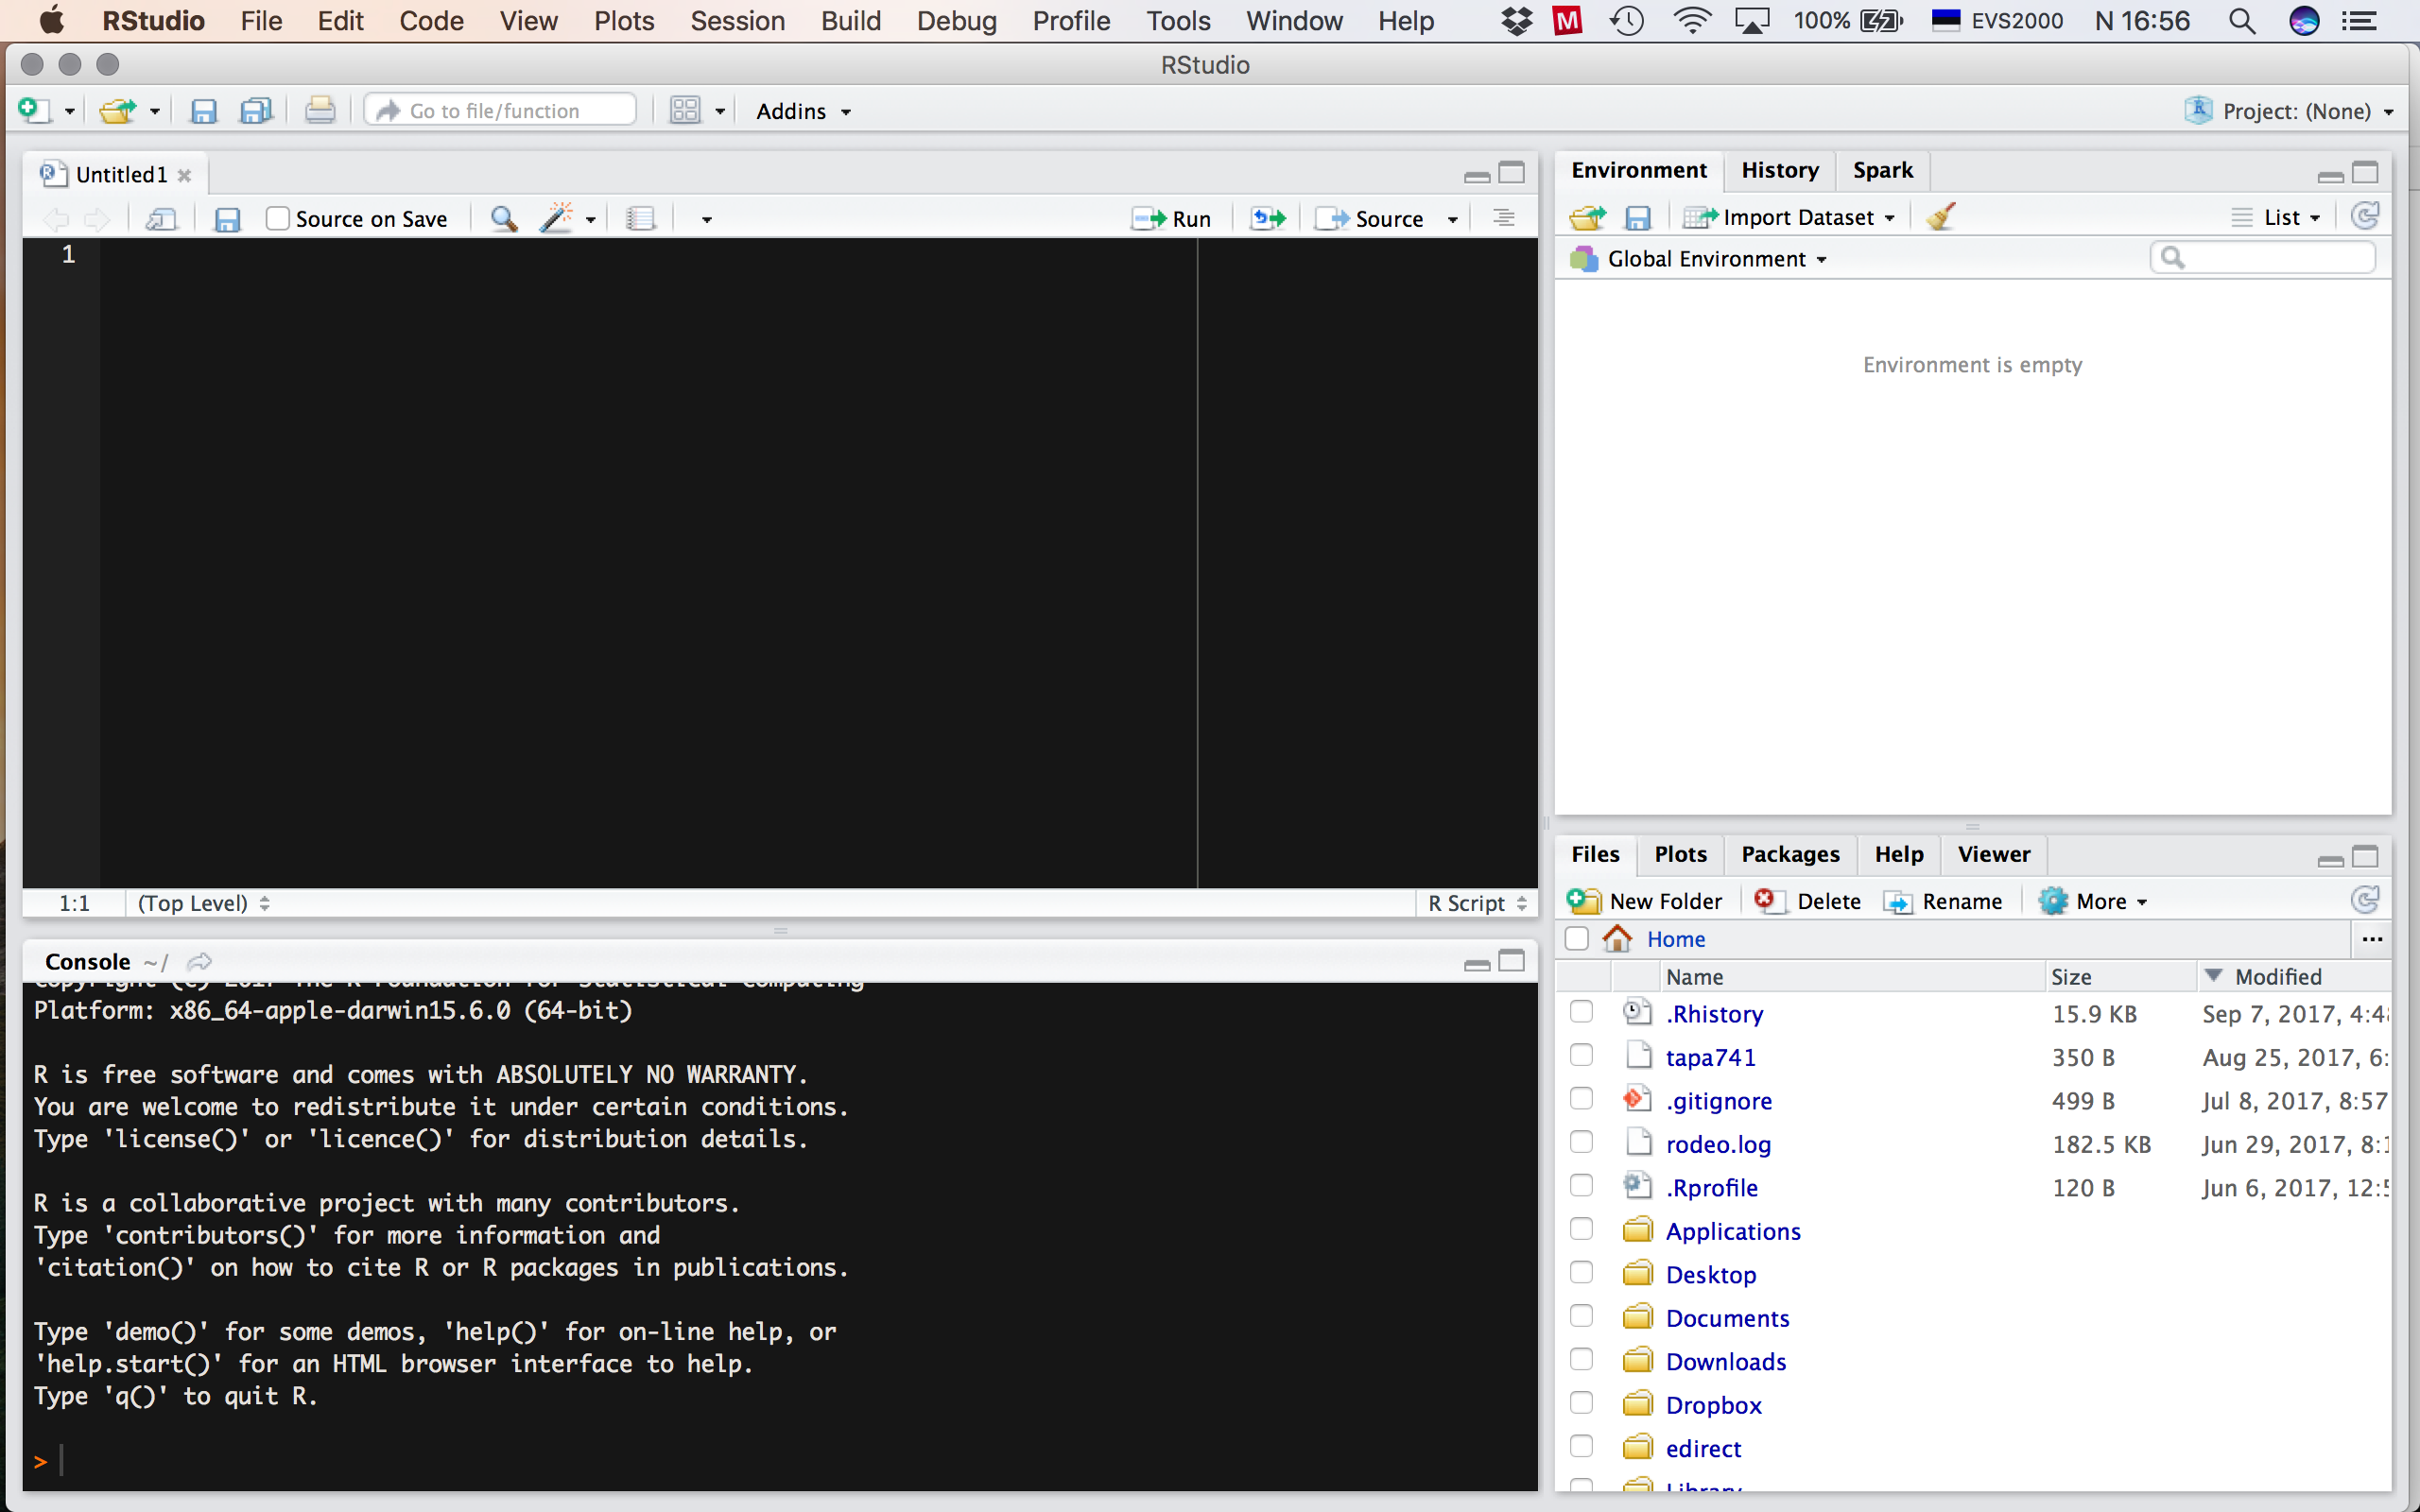
\includegraphics[width=35.56in]{assets/img/rstudio_screen_untitled} \caption{RStudio konsoolis on neli akent. Üleval vasakul on sinu poolt nimega varustatud koodi ja teksti editor kuhu kirjutad R skripti. Sinna kirjutad oma koodi ja kommentaarid sellele. All vasakul on konsool. Sinna sisestatakse käivitamisel sinu R kood ja sinna trükitakse väljund. Üleval paremal on Environment aken olulise sakiga <i class='fa fa-git' aria-hidden='true'></i>. Seal on näha R-i objektid, mis on sulle töökeskkonnas kättesaadavad ja millega sa saad töötada. <i class='fa fa-git' aria-hidden='true'></i> menüüs on võimalik muutusi vaadata ja 'commit'ida ja <i class='fa fa-github' aria-hidden='true'></i>-ga suhelda. All paremal on paneel mitme sakiga. Files tab töötab nagu failihaldur. Kui sa lood või avad R projekti, siis näidatakse seal vaikimisi sinu töökataloogi. Kui kasutad R projekti, siis ei ole vaja töökataloogi eraldi seadistada. Plots paneelile ilmuvad joonised, mille sa teed. Packages näitab sulle sinu arvutis olevaid R-i pakette ehk raamatukogusid. Help paneeli avanevad help failid (ka need, mida konsooli kaudu otsitakse).}\label{fig:rstudiowindow}
\end{figure}

Rohkem infot R projekti loomise kohta leiad RStudio infoleheküljelt:
\href{https://support.rstudio.com/hc/en-us/articles/200526207-Using-Projects}{Using
Projects}.

\section{\texorpdfstring{Git \emph{Merge}
konfliktid}{Git Merge konfliktid}}\label{git-merge-konfliktid}

Kollaboreerides üle GitHubi tekivad varem või hiljem konfliktid projekti
failide versioonide vahel nn. ``merge conflicts'', nende korrektselt
lahendama õppimine on väga oluline.

\begin{itemize}
\tightlist
\item
  Oma repo GitHubi veebilehel muuda/paranda README.md dokumenti ja
  ``Commit''-i seda lühisõnumiga mis sa muutsid/parandasid.
\item
  Seejärel, muuda oma arvutis olevat README.md faili RStudio-s viies
  sinna sisse mingi teistsuguse muudatuse. Tee ``Commit'' oma
  muudatustele.
\item
  Proovi ``push''-ida -- sa saad veateate!
\item
  Proovi ``pull''.
\item
  Lahenda ``merge'' konflikt ja seejärel ``commit'' + ``push''.
\end{itemize}

Githubi veateadete lugemine ja Google otsing aitavad sind.

\section{R projekti kataloogi soovitatav minimaalne
struktuur}\label{r-projekti-kataloogi-soovitatav-minimaalne-struktuur}

Iga R projekt peab olema täiesti iseseisev (\emph{selfcontained}) ja
sisaldama kogu infot, andmeid ja instruktsioone, et projektiga seotud
arvutused läbi viia ja raport genereerida. Kõik faili \emph{path}-id
peavad olema suhtelised.

R projekti kataloog peaks sisaldama projekti kirjeldavaid faile, mis
nimetatakse DESCRIPTION ja README.md. \textbf{DESCRIPTION} on tavaline
tekstifail ja sisaldab projekti metainfot ja infot projekti sõltuvuste
kohta, nagu väliste andmesettide asukoht, vajalik tarkvara jne.
\textbf{README.md} on markdown formaadis projekti info, sisaldab
juhendeid kasutajatele. Igale GitHubi repole on soovitav koostada
README.md, esialgu kasvõi projekti pealkiri ja üks kirjeldav lause.
README.md ja DESCRIPTION asuvad projekti juurkataloogis.

\begin{quote}
Projekti juurkataloogi jäävad ka kõik .Rmd laiendiga teksti ja analüüsi
tulemusi sisaldavad failid, millest genereeritakse lõplik
raport/dokument.
\end{quote}

Suuremad projektid, nagu näiteks teadusartikkel või raamat, võivad
sisaldada mitmeid Rmd faile ja võib tekkida kange kisatus need mõnda
alamkataloogi tõsta. Aga \texttt{knitr::knit()}, mis Rmarkdowni
markdowniks konverteerib, arvestab, et Rmd fail asub juurkataloogis ja
arvestab juurkataloogi suhtes ka failis olevaid \emph{path}-e teistele
failidele (näiteks ``data/my\_data.csv'').

\textbf{data/} kataloog sisaldab faile toorandmetega. Need failid peavad
olema R-i poolt loetavad ja soovitavalt tekstipõhised, laienditega TXT,
CSV, TSV jne. Neid faile ei muudeta, ainult loetakse. Kogu algandmete
töötlus toimub programmaatiliselt. Suured failid muudavad
versioonikontrolli aeglaseks, samuti on suheliselt mõttetu
versioonikontroll binaarsete failide korral (MS näiteks), sest diffid
pole lihtsalt inimkeeles. Github ütleb suurte failide kohta nii:
\emph{``GitHub will warn you when pushing files larger than 50 MB. You
will not be allowed to push files larger than 100 MB.''}

\textbf{src/} kataloog sisaldab analüüsi skripte, sealhulgas ka
andmetöötluse skripte.

\textbf{lib/} kataloogis on kasutaja poolt tehtud funktsioonide
definitsioone sisaldavad R skriptid.

\begin{verbatim}
project/
|- DESCRIPTION       # project metadata and dependencies
|- README.md         # description of contents and guide to users
|- my_analysis.Rmd   # markdown file containing analysis
|                    # writeup together with R code chunks
|
|- data/             # raw data, not changed once created 
|  +-my_data.csv     # data files in open formats, 
|                    # such as TXT, CSV, TSV etc.
|
|- src/              # any programmatic code
|  +-my_scripts.R    # R code used to analyse and 
|                    # visualise data
|
|- lib/              # user generated functions
|  +-my_functions.R  # R code defining functions
\end{verbatim}

On ka teisi konventsioone, näiteks R pakkide puhul paigutatakse kõik R
skriptid taaskasutatavate funktsioonidega kataloogi \textbf{R/}. Kui
selles kataloogis olevad skriptid on annoteeritud kasutades Roxygen-i
\citep{roxygen2}, siis genereeritakse automaatselt funktsioonide
dokumentatsioon kataloogi \textbf{man/}. Rohkem projekti pakkimise kohta
loe värskest preprindist ``Packaging data analytical work reproducibly
using R'' \citep{marwick2017}.

\section{Pakettide installeerimine}\label{libs}

R \emph{library}-d ehk paketid sisaldavad ühte või enamat mingit kindlat
operatsiooni läbi viivat funktsiooni. \textbf{R baaspakett sisaldab juba
mitmeid funktsioone.} Kõige esimene sõnum \texttt{sum()} help lehel on
``sum \{base\}'', mis tähendab, et see funktsioon kuulub nn.
baasfunktsioonide hulka. Need funktsioonid on alati kättesaadavad sest
neid sisaldavad raamatukogud laetakse vaikimisi teie töökeskkonda.
Näiteks ``base'' raamatukogu versioon 3.4.1 sisaldab 453 funktsiooni.
Enamasti on sarnaseid asju tegevad funktsioonid koondatud kokku
raamatukogudesse ehk pakettidesse, mis tuleb eraldi R kesksest
repositooriumist \href{https://cran.r-project.org}{CRAN} alla laadida ja
installeerida.

Selleks, et installeerida pakett, sisesta järgnev käsurida R konsooli:

\begin{Shaded}
\begin{Highlighting}[]
\NormalTok{## eg use "ggplot2" as packagename}
\KeywordTok{install.packages}\NormalTok{(}\StringTok{"packagename"}\NormalTok{)}
\end{Highlighting}
\end{Shaded}

NB! Kui mõni raamatukogu sel viisil alla ei tule, siis guugeldage selle
nime + R ja vaadake instruktsioone installeerimiseks. Suure tõenäosusega
on tegemist mõnes teises repos (näiteks Bioconductor) või ainult
GitHubis asuva paketiga.

RStudio võimaldab ka \emph{point-and-click} stiilis pakettide
installeerimist:

\begin{figure}
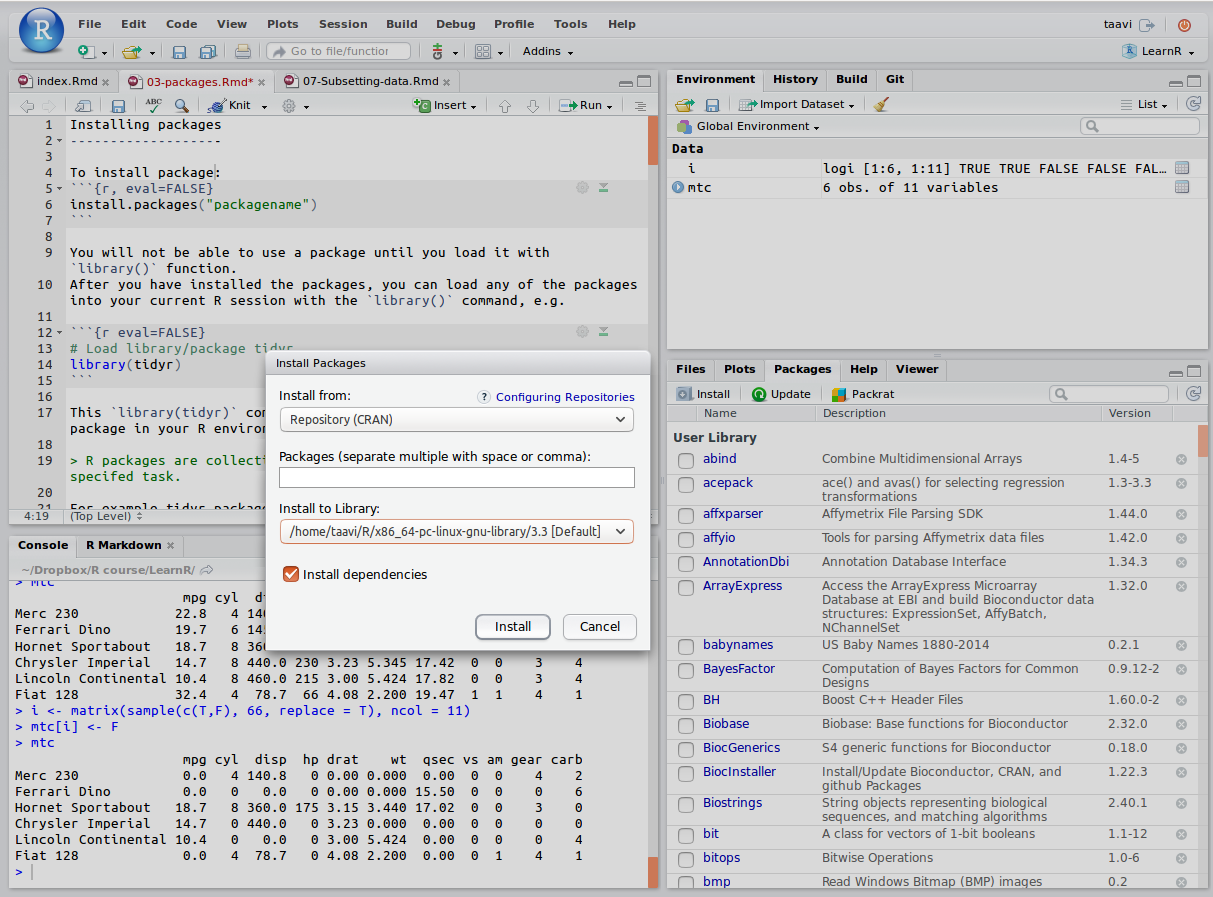
\includegraphics[width=16.85in]{assets/img/RStudio_package.install} \caption{RStudio 'Install Packages' dialoogiaken.}\label{fig:unnamed-chunk-2}
\end{figure}

\begin{quote}
Sa ei saa installeeritud pakette enne kasutada, kui laadid nad
töökeskkonda kasutades \texttt{library()} funktsiooni.
\end{quote}

Peale installeerimist lae pakett oma R sessiooni kasutades
\texttt{library()} käsku, näiteks:

\begin{Shaded}
\begin{Highlighting}[]
\NormalTok{## Load library/package tidyr}
\KeywordTok{library}\NormalTok{(dplyr)}
\end{Highlighting}
\end{Shaded}

\texttt{library(dplyr)} käsk teeb R sessioonis kasutatavaks kõik
``dplyr'' paketi funktsioonid.

Näiteks ``dplyr'' pakett sisaldab 237 funktsiooni:

\begin{Shaded}
\begin{Highlighting}[]
\KeywordTok{library}\NormalTok{(dplyr)}
\NormalTok{## let's look at the head of package list}
\KeywordTok{head}\NormalTok{(}\KeywordTok{ls}\NormalTok{(}\StringTok{"package:dplyr"}\NormalTok{), }\DecValTok{20}\NormalTok{)}
\end{Highlighting}
\end{Shaded}

\begin{verbatim}
##  [1] "%>%"           "add_count"     "add_count_"    "add_row"      
##  [5] "add_rownames"  "add_tally"     "add_tally_"    "all_equal"    
##  [9] "all_vars"      "anti_join"     "any_vars"      "arrange"      
## [13] "arrange_"      "arrange_all"   "arrange_at"    "arrange_if"   
## [17] "as_data_frame" "as_tibble"     "as.tbl"        "as.tbl_cube"
\end{verbatim}

Konfliktide korral eri pakettide sama nimega funktsioonide vahel saab
\texttt{::} operaatorit kasutades kutsuda välja/importida funktsiooni
spetsiifilisest paketist:

\begin{Shaded}
\begin{Highlighting}[]
\NormalTok{dplyr}\OperatorTok{::}\KeywordTok{select}\NormalTok{(df, my_var)}
\end{Highlighting}
\end{Shaded}

Sellisel kujul funktsioonide kasutamisel pole vaja imporditavat
funktsiooni sisaldavat raamatukogu töökeskkonda laadida.

\textbf{Funktsioonide-pakettide help failid RStudio kasutajaliidesest}:
Kui te lähete RStudios paremal all olevale ``Packages'' tabile, siis on
võimalik klikkida raamatukogu nimele ja näha selle help-faile,
tutooriale ja kõiki selle raamatukogu funktsioone koos nende help
failidega.

\section{R repositooriumid}\label{r-repositooriumid}

R pakid on saadaval kolmest põhilisest repositooriumist:

\begin{enumerate}
\def\labelenumi{\arabic{enumi}.}
\tightlist
\item
  \textbf{CRAN} \url{https://cran.r-project.org}
\end{enumerate}

\begin{Shaded}
\begin{Highlighting}[]
\KeywordTok{install.packages}\NormalTok{(}\StringTok{"ggplot2"}\NormalTok{)}
\end{Highlighting}
\end{Shaded}

\begin{enumerate}
\def\labelenumi{\arabic{enumi}.}
\setcounter{enumi}{1}
\tightlist
\item
  \textbf{Bioconductor} \url{https://www.bioconductor.org}
\end{enumerate}

\begin{Shaded}
\begin{Highlighting}[]
\CommentTok{# First run biocLite script fron bioconductor.org}
\KeywordTok{source}\NormalTok{(}\StringTok{"https://bioconductor.org/biocLite.R"}\NormalTok{)  }
\CommentTok{# use 'http' in url if 'https' is unavailable. }
\KeywordTok{biocLite}\NormalTok{(}\StringTok{"GenomicRanges"}\NormalTok{, }\DataTypeTok{suppressUpdates =} \OtherTok{TRUE}\NormalTok{)}
\end{Highlighting}
\end{Shaded}

\begin{enumerate}
\def\labelenumi{\arabic{enumi}.}
\setcounter{enumi}{2}
\tightlist
\item
  \textbf{GitHub} \url{https://github.com}
\end{enumerate}

\begin{Shaded}
\begin{Highlighting}[]
\NormalTok{## Näiteks järgnev käsk installeerib xaringan }
\NormalTok{## presentation ninja paketi}
\NormalTok{devtools}\OperatorTok{::}\KeywordTok{install_github}\NormalTok{(}\StringTok{"yihui/xaringan"}\NormalTok{)}
\end{Highlighting}
\end{Shaded}

\begin{quote}
NB! antud praktilise kursuse raames tutvume ja kasutame `tidyverse'
metapaketi funktsioone, laadides need iga sessiooni alguses:
\end{quote}

\begin{Shaded}
\begin{Highlighting}[]
\NormalTok{## install.packages("tidyverse")}
\KeywordTok{library}\NormalTok{(tidyverse)}
\end{Highlighting}
\end{Shaded}

Nüüd on teil \texttt{tidyverse} pakett arvutis. Tegelikult kuuluvad siia
raamatukokku omakorda tosinkond raamatukogu --- tidyverse on pisut meta.
Igal juhul muutuvad selle funktsioonid kättesaadavaks peale seda, kui te
need töökeskkonda sisse loete

Veel üks tehniline detail. \texttt{library(tidyverse)} käsk ei loe sisse
kõiki alam-raamatukogusid, mis selle nime all CRAN-ist alla laaditi.
Need tuleb vajadusel eraldi ükshaaval sisse lugeda.

\begin{quote}
Paiguta kõigi raamatukogude lugemine koodi algusesse. Enamasti
kirjutatakse sisse loetavad raamatukogud kohe R scripti algusesse. Siis
on teile endale ja teistele kes teie koodi loevad ilusti näha, mida
hiljem vaja läheb.
\end{quote}

\chapter{R on kalkulaator}\label{calc}

Liidame \texttt{2\ +\ 2}.

\begin{Shaded}
\begin{Highlighting}[]
\DecValTok{2} \OperatorTok{+}\StringTok{ }\DecValTok{2}
\end{Highlighting}
\end{Shaded}

\begin{verbatim}
## [1] 4
\end{verbatim}

Nüüd trükiti see vastus konsooli kujul \texttt{{[}1{]}\ 4}. See
tähendab, et \texttt{2\ +\ 2\ =\ 4}.

Kontrollime seda:

\begin{Shaded}
\begin{Highlighting}[]
\NormalTok{## liidame 2 ja 2 ning vaatame kas vastus võrdub 4}
\NormalTok{answer <-}\StringTok{ }\NormalTok{(}\DecValTok{2} \OperatorTok{+}\StringTok{ }\DecValTok{2}\NormalTok{) }\OperatorTok{==}\StringTok{ }\DecValTok{4}
\NormalTok{## Trükime vastuse välja}
\NormalTok{answer}
\end{Highlighting}
\end{Shaded}

\begin{verbatim}
## [1] TRUE
\end{verbatim}

Vastus on TRUE, (logical).

Pane tähele, et aritmeetiline võrdusmärk on \texttt{==} (sest = tähendab
hoopis väärtuse määramist objektile/argumendile).

Veel mõned näidisarvutused:

\begin{Shaded}
\begin{Highlighting}[]
\NormalTok{## 3 astmes 2; Please read Note ?'**' }
\DecValTok{3} \OperatorTok{^}\StringTok{ }\DecValTok{2}
\NormalTok{## Ruutjuur 3st}
\KeywordTok{sqrt}\NormalTok{(}\DecValTok{3}\NormalTok{)}
\NormalTok{## Naturaallogaritm sajast}
\KeywordTok{log}\NormalTok{(}\DecValTok{100}\NormalTok{)}
\end{Highlighting}
\end{Shaded}

Arvule \(\pi\) on määratud oma objekt \texttt{pi}. Seega on soovitav
enda poolt loodavatele objektidele mitte panna nimeks ``pi''.

\begin{Shaded}
\begin{Highlighting}[]
\NormalTok{## Ümarda pi neljale komakohale}
\KeywordTok{round}\NormalTok{(pi, }\DecValTok{4}\NormalTok{)}
\end{Highlighting}
\end{Shaded}

\begin{verbatim}
## [1] 3.1416
\end{verbatim}

Ümardamine on oluline tulemuste väljaprintimisel.

\section{Sama koodi saab kirjutada neljal
viisil}\label{sama-koodi-saab-kirjutada-neljal-viisil}

Hargnevate teede aed: kui me muudame olemasolevat objekti on meil alati
kaks valikut. Me kas jätame muudetud objektile vana objekti nime või me
anname talle uue nime. Esimesel juhul läheb vana muutmata objekt
workspacest kaduma aga nimesid ei tule juurde ja säilib teatud workflow
sujuvus. Teisel juhul jäävad analüüsi vaheobjektid meile alles ja nende
juurde saab alati tagasi tulla. Samas tekkib meile palju sarnaste
nimedega objekte.

Esimnene võimalus:

\begin{Shaded}
\begin{Highlighting}[]
\NormalTok{a <-}\StringTok{ }\KeywordTok{c}\NormalTok{(}\DecValTok{2}\NormalTok{, }\DecValTok{3}\NormalTok{)}
\NormalTok{a <-}\StringTok{ }\KeywordTok{sum}\NormalTok{(a)}
\NormalTok{a <-}\StringTok{ }\KeywordTok{sqrt}\NormalTok{(a)}
\NormalTok{a <-}\StringTok{ }\KeywordTok{round}\NormalTok{(a, }\DecValTok{2}\NormalTok{)}
\NormalTok{a}
\end{Highlighting}
\end{Shaded}

\begin{verbatim}
## [1] 2.24
\end{verbatim}

Teine võimalus:

\begin{Shaded}
\begin{Highlighting}[]
\NormalTok{a <-}\StringTok{ }\KeywordTok{c}\NormalTok{(}\DecValTok{2}\NormalTok{, }\DecValTok{3}\NormalTok{)}
\NormalTok{a1 <-}\StringTok{ }\KeywordTok{sum}\NormalTok{(a)}
\NormalTok{a2 <-}\StringTok{ }\KeywordTok{sqrt}\NormalTok{(a1)}
\NormalTok{a3 <-}\StringTok{ }\KeywordTok{round}\NormalTok{(a2, }\DecValTok{2}\NormalTok{)}
\NormalTok{a3}
\end{Highlighting}
\end{Shaded}

\begin{verbatim}
## [1] 2.24
\end{verbatim}

Kolmas võimalus on lühem variant esimesest. Me nimelt ühendame etapid
toru \texttt{\%\textgreater{}\%} kaudu. Siin me võtame objekti ``a''
(nö. andmed), suuname selle funktsiooni \texttt{sum()}, võtame selle
funktsiooni väljundi ja suuname selle omakorda funktsiooni
\texttt{sqrt()}. Seejärel võtame selle funktsiooni outputi ja määrame
selle nimele ``result'' (aga võime selle ka mõne teise nimega siduda).
Kui mõni funktsioon võtab ainult ühe parameetri, mille me talle toru
kaudu sisse sõõdame, siis pole selle funktsiooni taga isegi sulge vaja.

\begin{quote}
NB! R hea stiili juhised soovitavad siiski ka \emph{pipe}-s kasutada
funktsiooni koos sulgudega!
\end{quote}

See on hea lühike ja inimloetav viis koodi kirjutada, mis on masina
jaoks identne esimese koodiga.

\begin{Shaded}
\begin{Highlighting}[]
\NormalTok{## we need piping operator '%>%' from magrittr}
\KeywordTok{library}\NormalTok{(magrittr)}
\NormalTok{a <-}\StringTok{ }\KeywordTok{c}\NormalTok{(}\DecValTok{2}\NormalTok{, }\DecValTok{3}\NormalTok{)}
\NormalTok{result <-}\StringTok{ }\NormalTok{a }\OperatorTok\StringTok{ }\KeywordTok{sum}\NormalTok{() }\OperatorTok\StringTok{ }\KeywordTok{sqrt}\NormalTok{() }\OperatorTok\StringTok{ }\KeywordTok{round}\NormalTok{(}\DecValTok{2}\NormalTok{)}
\NormalTok{result}
\end{Highlighting}
\end{Shaded}

\begin{verbatim}
## [1] 2.24
\end{verbatim}

Neljas võimalus, klassikaline baas R lahendus:

\begin{Shaded}
\begin{Highlighting}[]
\NormalTok{a <-}\StringTok{ }\KeywordTok{c}\NormalTok{(}\DecValTok{2}\NormalTok{, }\DecValTok{3}\NormalTok{)}
\NormalTok{a1 <-}\StringTok{ }\KeywordTok{round}\NormalTok{(}\KeywordTok{sqrt}\NormalTok{(}\KeywordTok{sum}\NormalTok{(a)), }\DecValTok{2}\NormalTok{)}
\NormalTok{a1}
\end{Highlighting}
\end{Shaded}

\begin{verbatim}
## [1] 2.24
\end{verbatim}

Sellist koodi loetakse keskelt väljappoole ja kirjutatakse alates
viimasest operatsioonist, mida soovitakse, et kood teeks. Masina jaoks
pole vahet. Inimese jaoks on küll: 4. variant nõuab hästi pestud ajusid.

Koodi lühidus 4 --\textgreater{} 3 --\textgreater{} 1 --\textgreater{} 2
(pikem) Lollikindlus 1 --\textgreater{} 2 --\textgreater{} 3
--\textgreater{} 4 (vähem lollikindel)

See on teie otsustada, millist koodivormi te millal kasutate, aga te
peaksite oskama lugeda neid kõiki.

\chapter{R objektid}\label{obj}

R-i töökeskkonnas ``workspace'' asuvad \textbf{objektid}, millega me
töötame. Tüüpilised objektid on:

\begin{itemize}
\tightlist
\item
  Vektorid, maatriksid, listid ja tabelid.
\item
  Statistiliste analüüside väljundid (S3, S4 klass).
\item
  Funktsioonid, mille oleme ise sisse lugenud.
\end{itemize}

Käsk \texttt{ls()} annab objektide nimed teie workspace-s:

\begin{Shaded}
\begin{Highlighting}[]
\KeywordTok{ls}\NormalTok{()}
\end{Highlighting}
\end{Shaded}

\begin{verbatim}
## [1] "a"      "a1"     "a2"     "a3"     "answer" "result"
\end{verbatim}

\texttt{rm(a)} removes object a from the workspace

Selleks, et salvestada töökeskkond faili kasuta ``Save'' nuppu
``Environment'' akna servast või menüüst ``Session'' -\textgreater{}
``Save Workspace As''.

Projekti sulgemisel salvestab RStudio vaikimisi töökeskkonna.
\textbf{Parema reprodutseeritavuse huvides pole siiski soovitav
töökeskkonda peale töö lõppu projekti sulgemisel salvestada!}. Lülitame
automaatse salvestamise välja:

\begin{itemize}
\tightlist
\item
  Selleks mine ``Tools'' \textgreater{} ``Global Options''
  \textgreater{} kõige ülemine, ``R General'' menüüs vali ``Save
  workspace to .RData on exit'' \textgreater{} ``Never'' ever!
\item
  Võta ära linnuke ``Restore .RData to workspace at startup'' eest.
\end{itemize}

Kui on mingid kaua aega võtvad kalkulatsioonid või allalaadimised
salvesta need eraldi .rds faili ja laadi koodis vastavalt vajadusele.

\section{Objekt ja nimi}\label{objekt-ja-nimi}

Kui teil sünnib laps, annate talle nime.

R-s on vastupidi: nimele antakse objekt

\begin{Shaded}
\begin{Highlighting}[]
\NormalTok{babe <-}\StringTok{ "beebi"}
\NormalTok{babe}
\end{Highlighting}
\end{Shaded}

\begin{verbatim}
## [1] "beebi"
\end{verbatim}

Siin on kõigepealt nimi (babe), siis assingmenti sümbol
\texttt{\textless{}-} ja lõpuks objekt, mis on nimele antud (string
``beebi'').

NB! Stringid on jutumärkides, nimed mitte. Nimi üksi evalueeritakse kui
``print object'', mis antud juhul on string ``beebi''

Nüüd muudame objekti nime taga:

\begin{Shaded}
\begin{Highlighting}[]
\NormalTok{babe <-}\StringTok{ }\KeywordTok{c}\NormalTok{(}\StringTok{"saatan"}\NormalTok{, }\StringTok{"inglike"}\NormalTok{)}
\NormalTok{babe}
\end{Highlighting}
\end{Shaded}

\begin{verbatim}
## [1] "saatan"  "inglike"
\end{verbatim}

Tulemuseks on sama nimi, mis tähistab nüüd midagi muud (vektorit, mis
koosneb 2st stringist). Objekt ``beebi'' kaotas oma nime ja on nüüd
workspacest kadunud. \texttt{class()} annab meile objekti klassi.

\begin{Shaded}
\begin{Highlighting}[]
\KeywordTok{class}\NormalTok{(babe)}
\end{Highlighting}
\end{Shaded}

\begin{verbatim}
## [1] "character"
\end{verbatim}

Antud juhul character.

\begin{quote}
Ainult need objektid, mis on assigneeritud nimele, lähevad workspace ja
on sellistena kasutatvad edasises analüüsis.
\end{quote}

\begin{Shaded}
\begin{Highlighting}[]
\NormalTok{apples <-}\StringTok{ }\DecValTok{2}
\NormalTok{bananas <-}\StringTok{ }\DecValTok{3}
\NormalTok{apples }\OperatorTok{+}\StringTok{ }\NormalTok{bananas}
\end{Highlighting}
\end{Shaded}

\begin{verbatim}
## [1] 5
\end{verbatim}

Selle ekspressiooni tulemus trükitakse ainult R konsooli, kuna teda ei
määrata nimele siis ei ilmu see ka workspace.

\begin{Shaded}
\begin{Highlighting}[]
\NormalTok{a <-}\StringTok{ }\DecValTok{2}
\NormalTok{b <-}\StringTok{ }\DecValTok{3}
\NormalTok{a <-}\StringTok{ }\NormalTok{a }\OperatorTok{+}\StringTok{ }\NormalTok{b}
\CommentTok{# objekti nimega 'a' struktuur}
\KeywordTok{str}\NormalTok{(a)}
\end{Highlighting}
\end{Shaded}

\begin{verbatim}
##  num 5
\end{verbatim}

Nüüd on nimega a seostatud uus objekt, mis sisaldab numbrit 5 (olles ühe
elemendiga vektor). Ja nimega a eelnevalt seostatud objekt, mis koosnes
numbrist 2, on workspacest lahkunud.

\section{Nimede vorm}\label{nimede-vorm}

\begin{itemize}
\tightlist
\item
  Nimed algavad tähemärgiga, mitte numbriga ega
  \$\euro{}\%\&/?\textasciitilde{}ˇöõüä
\item
  Nimed ei sisalda tühikuid
\item
  Tühiku asemel kasuta alakriipsu: näiteks eriti\_pikk\_nimi
\item
  SUURED ja väiksed tähed on nimes erinevad
\item
  Nimed peaksid kirjeldama objekti, mis on sellele nimele assigneeritud
  ja nad võivad olla pikad sest TAB klahv annab meile auto-complete.
\item
  alt + - on otsetee \texttt{\textless{}-} jaoks
\end{itemize}

\section{Andmete tüübid}\label{andmete-tuubid}

\begin{itemize}
\tightlist
\item
  numeric / integer
\item
  logical -- 2 väärtust TRUE/FALSE
\item
  character
\item
  factor (ordered and unordered) - 2+ diskreetset väärtust, mis võivad
  olla järjestatud suuremast väiksemani (aga ei asu üksteisest võrdsel
  kaugusel). Faktoreid käsitleme põhjalikumalt hiljem.
\end{itemize}

Andmete tüüpe saab üksteiseks konverteerida \texttt{as.numeric()},
\texttt{as.character()}, \texttt{as.factor()}.

\section{Vektor}\label{vektor}

Vektor on rida kindlas järjekorras arve, sõnu või TRUE/FALSE loogilisi
väärtusi. Iga vektor ja maatriks (2D vektor) sisaldab ainult ühte tüüpi
andmeid. Vektor on elementaarüksus, millega me teeme tehteid.
Andmetabelis ripuvad kõrvuti ühepikad vektorid (üks vektor = üks tulp)
ja R-le meeldib arvutada vektori kaupa vasakult paremale (mis tabelis on
ülevalt alla sest vektori algus on üleval tabeli peas). Pikema kui
üheelemendise vektori loomiseks kasuta funktsiooni \texttt{c()} --
combine

Loome numbrilise vektori ja vaatame ta struktuuri:

\begin{Shaded}
\begin{Highlighting}[]
\NormalTok{minu_vektor <-}\StringTok{ }\KeywordTok{c}\NormalTok{(}\DecValTok{1}\NormalTok{, }\DecValTok{3}\NormalTok{, }\DecValTok{4}\NormalTok{)}
\KeywordTok{str}\NormalTok{(minu_vektor)}
\end{Highlighting}
\end{Shaded}

\begin{verbatim}
##  num [1:3] 1 3 4
\end{verbatim}

Loome vektori puuduva väärtusega, vaatame vektori klassi:

\begin{Shaded}
\begin{Highlighting}[]
\NormalTok{minu_vektor <-}\StringTok{ }\KeywordTok{c}\NormalTok{(}\DecValTok{1}\NormalTok{, }\OtherTok{NA}\NormalTok{, }\DecValTok{4}\NormalTok{)}
\NormalTok{minu_vektor}
\end{Highlighting}
\end{Shaded}

\begin{verbatim}
## [1]  1 NA  4
\end{verbatim}

\begin{Shaded}
\begin{Highlighting}[]
\KeywordTok{class}\NormalTok{(minu_vektor)}
\end{Highlighting}
\end{Shaded}

\begin{verbatim}
## [1] "numeric"
\end{verbatim}

Klass jääb \emph{numeric}-uks.

Kui vektoris on segamini numbrid ja stringid, siis muudetakse numbrid ka
stringideks:

\begin{Shaded}
\begin{Highlighting}[]
\NormalTok{minu_vektor <-}\StringTok{ }\KeywordTok{c}\NormalTok{(}\DecValTok{1}\NormalTok{, }\StringTok{"2"}\NormalTok{, }\DecValTok{2}\NormalTok{, }\DecValTok{4}\NormalTok{, }\StringTok{"joe"}\NormalTok{)}
\NormalTok{minu_vektor}
\end{Highlighting}
\end{Shaded}

\begin{verbatim}
## [1] "1"   "2"   "2"   "4"   "joe"
\end{verbatim}

\begin{Shaded}
\begin{Highlighting}[]
\KeywordTok{class}\NormalTok{(minu_vektor)}
\end{Highlighting}
\end{Shaded}

\begin{verbatim}
## [1] "character"
\end{verbatim}

Piisab ühest ``tõrvatilgast meepotis'', et teie vektor ei sisaldaks enam
numbreid.

Eelnevast segavektorist on võimalik numbrid päästa kasutades käsku
\texttt{as.numeric()}:

\begin{Shaded}
\begin{Highlighting}[]
\KeywordTok{as.numeric}\NormalTok{(minu_vektor)}
\end{Highlighting}
\end{Shaded}

\begin{verbatim}
## Warning: NAs introduced by coercion
\end{verbatim}

\begin{verbatim}
## [1]  1  2  2  4 NA
\end{verbatim}

Väärtus ``joe'' muudeti NA-ks, kuna seda ei olnud võimalik numbriks
muuta. Samuti peab olema tähelepanelik faktorite muutmisel numbriteks:

\begin{Shaded}
\begin{Highlighting}[]
\NormalTok{minu_vektor <-}\StringTok{ }\KeywordTok{factor}\NormalTok{(}\KeywordTok{c}\NormalTok{(}\DecValTok{9}\NormalTok{, }\StringTok{"12"}\NormalTok{, }\DecValTok{12}\NormalTok{, }\FloatTok{1.4}\NormalTok{, }\StringTok{"joe"}\NormalTok{))}
\NormalTok{minu_vektor}
\end{Highlighting}
\end{Shaded}

\begin{verbatim}
## [1] 9   12  12  1.4 joe
## Levels: 1.4 12 9 joe
\end{verbatim}

\begin{Shaded}
\begin{Highlighting}[]
\KeywordTok{class}\NormalTok{(minu_vektor)}
\end{Highlighting}
\end{Shaded}

\begin{verbatim}
## [1] "factor"
\end{verbatim}

\begin{Shaded}
\begin{Highlighting}[]
\NormalTok{## Kui muudame faktori otse numbriks, saame faktori taseme numbri}
\KeywordTok{as.numeric}\NormalTok{(minu_vektor)}
\end{Highlighting}
\end{Shaded}

\begin{verbatim}
## [1] 3 2 2 1 4
\end{verbatim}

Faktorite muutmisel numbriteks tuleb need kõigepealt stringideks muuta:

\begin{Shaded}
\begin{Highlighting}[]
\KeywordTok{as.numeric}\NormalTok{(}\KeywordTok{as.character}\NormalTok{(minu_vektor))}
\end{Highlighting}
\end{Shaded}

\begin{verbatim}
## Warning: NAs introduced by coercion
\end{verbatim}

\begin{verbatim}
## [1]  9.0 12.0 12.0  1.4   NA
\end{verbatim}

Järgneva trikiga saab stringidest ekstraheerida numbrid:

\begin{Shaded}
\begin{Highlighting}[]
\KeywordTok{library}\NormalTok{(readr)}
\NormalTok{minu_vektor <-}\StringTok{ }\KeywordTok{c}\NormalTok{(}\DecValTok{1}\NormalTok{, }\StringTok{"A2"}\NormalTok{, }\StringTok{"$2"}\NormalTok{, }\StringTok{"joe"}\NormalTok{)}
\NormalTok{minu_vektor <-}\StringTok{ }\KeywordTok{as.vector}\NormalTok{(}\KeywordTok{parse_number}\NormalTok{(minu_vektor))}
\end{Highlighting}
\end{Shaded}

\begin{verbatim}
## Warning: 1 parsing failure.
## row # A tibble: 1 x 4 col     row   col expected actual expected   <int> <int>    <chr>  <chr> actual 1     4    NA a number    joe
\end{verbatim}

\begin{Shaded}
\begin{Highlighting}[]
\NormalTok{minu_vektor}
\end{Highlighting}
\end{Shaded}

\begin{verbatim}
## [1]  1  2  2 NA
\end{verbatim}

\begin{Shaded}
\begin{Highlighting}[]
\KeywordTok{str}\NormalTok{(minu_vektor)}
\end{Highlighting}
\end{Shaded}

\begin{verbatim}
##  num [1:4] 1 2 2 NA
\end{verbatim}

R säilitab vektori algse järjekorra. Sageli on aga vaja tulemusi näiteks
vaatamiseks ja presenteerimiseks sorteerida suuruse või tähestiku
järjekorras:

\begin{Shaded}
\begin{Highlighting}[]
\NormalTok{## sorts vector in ascending order}
\KeywordTok{sort}\NormalTok{(x, }\DataTypeTok{decreasing =} \OtherTok{FALSE}\NormalTok{, ...)}
\end{Highlighting}
\end{Shaded}

Vektori unikaalsed väärtused saab kätte käsuga \texttt{unique()}:

\begin{Shaded}
\begin{Highlighting}[]
\NormalTok{## returns a vector or data frame, but with duplicate elements/rows removed}
\KeywordTok{unique}\NormalTok{(}\KeywordTok{c}\NormalTok{(}\DecValTok{1}\NormalTok{,}\DecValTok{1}\NormalTok{,}\DecValTok{1}\NormalTok{,}\DecValTok{2}\NormalTok{,}\DecValTok{2}\NormalTok{,}\DecValTok{2}\NormalTok{,}\DecValTok{2}\NormalTok{,}\DecValTok{2}\NormalTok{,}\DecValTok{3}\NormalTok{,}\DecValTok{3}\NormalTok{,}\DecValTok{4}\NormalTok{,}\DecValTok{5}\NormalTok{,}\DecValTok{5}\NormalTok{))}
\end{Highlighting}
\end{Shaded}

\begin{verbatim}
## [1] 1 2 3 4 5
\end{verbatim}

\subsection{\texorpdfstring{Uus vektor: \texttt{seq()} ja
\texttt{rep()}}{Uus vektor: seq() ja rep()}}\label{uus-vektor-seq-ja-rep}

\begin{Shaded}
\begin{Highlighting}[]
\KeywordTok{seq}\NormalTok{(}\DecValTok{2}\NormalTok{, }\DecValTok{3}\NormalTok{, }\DataTypeTok{by =} \FloatTok{0.5}\NormalTok{)}
\end{Highlighting}
\end{Shaded}

\begin{verbatim}
## [1] 2.0 2.5 3.0
\end{verbatim}

\begin{Shaded}
\begin{Highlighting}[]
\KeywordTok{seq}\NormalTok{(}\DecValTok{2}\NormalTok{, }\DecValTok{3}\NormalTok{, }\DataTypeTok{length.out =} \DecValTok{5}\NormalTok{)}
\end{Highlighting}
\end{Shaded}

\begin{verbatim}
## [1] 2.00 2.25 2.50 2.75 3.00
\end{verbatim}

\begin{Shaded}
\begin{Highlighting}[]
\KeywordTok{rep}\NormalTok{(}\DecValTok{1}\OperatorTok{:}\DecValTok{2}\NormalTok{, }\DataTypeTok{times =} \DecValTok{3}\NormalTok{)}
\end{Highlighting}
\end{Shaded}

\begin{verbatim}
## [1] 1 2 1 2 1 2
\end{verbatim}

\begin{Shaded}
\begin{Highlighting}[]
\KeywordTok{rep}\NormalTok{(}\DecValTok{1}\OperatorTok{:}\DecValTok{2}\NormalTok{, }\DataTypeTok{each =} \DecValTok{3}\NormalTok{)}
\end{Highlighting}
\end{Shaded}

\begin{verbatim}
## [1] 1 1 1 2 2 2
\end{verbatim}

\begin{Shaded}
\begin{Highlighting}[]
\KeywordTok{rep}\NormalTok{(}\KeywordTok{c}\NormalTok{(}\StringTok{"a"}\NormalTok{, }\StringTok{"b"}\NormalTok{), }\DataTypeTok{each =} \DecValTok{3}\NormalTok{, }\DataTypeTok{times =} \DecValTok{2}\NormalTok{)}
\end{Highlighting}
\end{Shaded}

\begin{verbatim}
##  [1] "a" "a" "a" "b" "b" "b" "a" "a" "a" "b" "b" "b"
\end{verbatim}

\subsection{Tehted arvuliste
vektoritega}\label{tehted-arvuliste-vektoritega}

Vektoreid saab liita, lahutada, korrutada ja jagada.

\begin{Shaded}
\begin{Highlighting}[]
\NormalTok{a <-}\StringTok{ }\KeywordTok{c}\NormalTok{(}\DecValTok{1}\NormalTok{, }\DecValTok{2}\NormalTok{, }\DecValTok{3}\NormalTok{)}
\NormalTok{b <-}\StringTok{ }\DecValTok{4}
\NormalTok{a }\OperatorTok{+}\StringTok{ }\NormalTok{b}
\end{Highlighting}
\end{Shaded}

\begin{verbatim}
## [1] 5 6 7
\end{verbatim}

Kõik vektor a liikmed liideti arvuga 3 (kuna vektor b koosnes ühest
liikmest, läks see kordusesse)

\begin{Shaded}
\begin{Highlighting}[]
\NormalTok{a <-}\StringTok{ }\KeywordTok{c}\NormalTok{(}\DecValTok{1}\NormalTok{, }\DecValTok{2}\NormalTok{, }\DecValTok{3}\NormalTok{)}
\NormalTok{b <-}\StringTok{ }\KeywordTok{c}\NormalTok{(}\DecValTok{4}\NormalTok{, }\DecValTok{5}\NormalTok{) }
\NormalTok{a }\OperatorTok{+}\StringTok{ }\NormalTok{b}
\end{Highlighting}
\end{Shaded}

\begin{verbatim}
## Warning in a + b: longer object length is not a multiple of shorter object
## length
\end{verbatim}

\begin{verbatim}
## [1] 5 7 7
\end{verbatim}

Aga see töötab veateatega, sest vektorite pikkused ei ole üksteise
kordajad 1 + 4; 2 + 5, 3 + 4

\begin{Shaded}
\begin{Highlighting}[]
\NormalTok{a <-}\StringTok{ }\KeywordTok{c}\NormalTok{(}\DecValTok{1}\NormalTok{, }\DecValTok{2}\NormalTok{, }\DecValTok{3}\NormalTok{, }\DecValTok{4}\NormalTok{)}
\NormalTok{b <-}\StringTok{ }\KeywordTok{c}\NormalTok{(}\DecValTok{5}\NormalTok{, }\DecValTok{6}\NormalTok{) }
\NormalTok{a }\OperatorTok{+}\StringTok{ }\NormalTok{b}
\end{Highlighting}
\end{Shaded}

\begin{verbatim}
## [1]  6  8  8 10
\end{verbatim}

See töötab: 1 + 5; 2 + 6; 3 + 5; 4 + 6

\begin{Shaded}
\begin{Highlighting}[]
\NormalTok{a <-}\StringTok{ }\KeywordTok{c}\NormalTok{(}\DecValTok{1}\NormalTok{, }\DecValTok{2}\NormalTok{, }\DecValTok{3}\NormalTok{, }\DecValTok{4}\NormalTok{)}
\NormalTok{b <-}\StringTok{ }\KeywordTok{c}\NormalTok{(}\DecValTok{5}\NormalTok{, }\DecValTok{6}\NormalTok{, }\DecValTok{7}\NormalTok{, }\DecValTok{8}\NormalTok{) }
\NormalTok{a }\OperatorTok{+}\StringTok{ }\NormalTok{b}
\end{Highlighting}
\end{Shaded}

\begin{verbatim}
## [1]  6  8 10 12
\end{verbatim}

Samuti see (ühepikkused vektorid --- igat liiget kasutatakse üks kord)

\begin{Shaded}
\begin{Highlighting}[]
\NormalTok{a <-}\StringTok{ }\KeywordTok{c}\NormalTok{(}\OtherTok{TRUE}\NormalTok{, }\OtherTok{FALSE}\NormalTok{, }\OtherTok{TRUE}\NormalTok{)}
\KeywordTok{sum}\NormalTok{(a)}
\end{Highlighting}
\end{Shaded}

\begin{verbatim}
## [1] 2
\end{verbatim}

\begin{Shaded}
\begin{Highlighting}[]
\KeywordTok{mean}\NormalTok{(a)}
\end{Highlighting}
\end{Shaded}

\begin{verbatim}
## [1] 0.6666667
\end{verbatim}

Mis siin juhtus? R kodeerib sisemiselt TRUE kui 1 ja FALSE kui 0-i.
summa 1 + 0 + 1 = 2. Seda loogiliste väärtuste omadust õpime varsti
praktikas kasutama.

\section{List}\label{list}

List on objektitüüp, kuhu saab koondada kõiki teisi objekte, kaasa
arvatud listid. See on lihtsalt viis objektid koos hoida ühes suuremas
meta-objektis. List on nagu jõuluvana kingikott, kus kommid, sokipaarid
ja muud kingid kõik segamini loksuvad.

Näiteks siin list, kus loksuvad 1 vektor nimega a, 1 tibble nimega b ja
1 list nimega c, mis omakorda sisaldab vektorit nimega d ja tibblet
nimega e. Seega on meil tegu rekursiivse listiga.

\begin{Shaded}
\begin{Highlighting}[]
\CommentTok{# numeric vector a}
\NormalTok{a <-}\StringTok{ }\KeywordTok{runif}\NormalTok{(}\DecValTok{5}\NormalTok{)}
\CommentTok{# data.frame}
\NormalTok{ab <-}\StringTok{ }\KeywordTok{data.frame}\NormalTok{(a, }\DataTypeTok{b =} \KeywordTok{rnorm}\NormalTok{(}\DecValTok{5}\NormalTok{))}
\CommentTok{# linear model}
\NormalTok{model <-}\StringTok{ }\KeywordTok{lm}\NormalTok{(mpg }\OperatorTok{~}\StringTok{ }\NormalTok{hp, }\DataTypeTok{data =}\NormalTok{ mtcars)}
\CommentTok{# your grandma on bongos}
\NormalTok{grandma <-}\StringTok{ "your grandma on bongos"}
\CommentTok{# let's creat list}
\NormalTok{happy_list <-}\StringTok{ }\KeywordTok{list}\NormalTok{(a, ab, model, grandma)}
\NormalTok{happy_list}
\end{Highlighting}
\end{Shaded}

\begin{verbatim}
## [[1]]
## [1] 0.01684116 0.92217625 0.83712493 0.57547763 0.80505060
## 
## [[2]]
##            a          b
## 1 0.01684116 -0.5035121
## 2 0.92217625 -0.4699207
## 3 0.83712493  1.7919783
## 4 0.57547763  0.5923619
## 5 0.80505060  2.0362937
## 
## [[3]]
## 
## Call:
## lm(formula = mpg ~ hp, data = mtcars)
## 
## Coefficients:
## (Intercept)           hp  
##    30.09886     -0.06823  
## 
## 
## [[4]]
## [1] "your grandma on bongos"
\end{verbatim}

Võtame listist välja elemndi ``ab'':

\begin{Shaded}
\begin{Highlighting}[]
\NormalTok{happy_list}\OperatorTok{$}\NormalTok{ab}
\end{Highlighting}
\end{Shaded}

\begin{verbatim}
## NULL
\end{verbatim}

\section{data frame ja tibble}\label{data-frame-ja-tibble}

\begin{Shaded}
\begin{Highlighting}[]
\KeywordTok{library}\NormalTok{(tidyverse)}
\end{Highlighting}
\end{Shaded}

Andmeraam on eriline list, mis koosneb ühepikkustest vektoritest.
Andmeraam on ühtlasi teatud liiki tabel, kus igas veerus on ainult ühte
tüüpi andmed. Need vektorid ripuvad andmeraamis kõrvuti nagu tuulehaugid
suitsuahjus, kusjuures vektori algus vastab tuulehaugi peale, mis on
konksu otsas (konks vastab andmeraamis tulba nimele ja ühtlasi vektori
nimele). Iga vektori nimi muutub sellises tabelis tulba nimeks. Igas
tulbas saab olla ainult ühte tüüpi andmeid.

R-s on 2 andmeraami tüüpi: data frame ja tibble, mis on väga sarnased.
Tibble on uuem, veidi kaunima väljatrükiga, pisut mugavam kasutada.

\begin{quote}
Oluline on, et erinevalt data frame-st saab tibblesse lisada ka list
tulpasid, mis võimaldab sisuliselt suvalisi R objekte tibblesse
paigutada. Põhimõtteliselt piisab ainult ühest andmestruktuurist --
tibble, et R-is töötada. Kõik mis juhtub tibbles jääb tibblesse. Nice
and tidy -- tidyverse.
\end{quote}

``Tidyverse'' töötab tibblega veidi paremini kui data frame-ga, aga see
vahe ei ole suur.

Siin on meil 3 vektorit: shop, apples ja oranges, millest me paneme
kokku tibble nimega fruits

\begin{Shaded}
\begin{Highlighting}[]
\NormalTok{## loome kolm vektorit}
\NormalTok{shop <-}\StringTok{ }\KeywordTok{c}\NormalTok{(}\StringTok{"maxima"}\NormalTok{, }\StringTok{"tesco"}\NormalTok{, }\StringTok{"lidl"}\NormalTok{)}
\NormalTok{apples <-}\StringTok{ }\KeywordTok{c}\NormalTok{(}\DecValTok{1}\NormalTok{, }\DecValTok{4}\NormalTok{, }\DecValTok{43}\NormalTok{)}
\NormalTok{oranges <-}\StringTok{ }\KeywordTok{c}\NormalTok{(}\DecValTok{2}\NormalTok{, }\DecValTok{32}\NormalTok{, }\OtherTok{NA}\NormalTok{)}
\NormalTok{vabakava <-}\StringTok{ }\KeywordTok{list}\NormalTok{(letters, }\KeywordTok{runif}\NormalTok{(}\DecValTok{10}\NormalTok{), }\KeywordTok{lm}\NormalTok{(mpg }\OperatorTok{~}\StringTok{ }\NormalTok{cyl, mtcars))}
\NormalTok{## paneme need vektorid kokku tibble-sse}
\NormalTok{fruits <-}\StringTok{ }\KeywordTok{tibble}\NormalTok{(shop, apples, oranges, vabakava)}
\NormalTok{fruits}
\end{Highlighting}
\end{Shaded}

\begin{verbatim}
## # A tibble: 3 x 4
##     shop apples oranges   vabakava
##    <chr>  <dbl>   <dbl>     <list>
## 1 maxima      1       2 <chr [26]>
## 2  tesco      4      32 <dbl [10]>
## 3   lidl     43      NA   <S3: lm>
\end{verbatim}

Siin ta on, ilusti meie workspace-s. Pange tähele viimast tulpa
``vabakava'', mis sisaldab \emph{character} vectorit, numbrilist
vektorit ja lineaarse mudeli objekti.

Listi juba nii lihtsalt data.frame-i ei pane:

\begin{Shaded}
\begin{Highlighting}[]
\KeywordTok{try}\NormalTok{(}\KeywordTok{data.frame}\NormalTok{(shop, apples, oranges, vabakava))}
\end{Highlighting}
\end{Shaded}

\textbf{Mõned asjad, mida tibblega (ja data framega) saab teha:}

\begin{Shaded}
\begin{Highlighting}[]
\KeywordTok{count}\NormalTok{(fruits, apples)}
\end{Highlighting}
\end{Shaded}

\begin{verbatim}
## # A tibble: 3 x 2
##   apples     n
##    <dbl> <int>
## 1      1     1
## 2      4     1
## 3     43     1
\end{verbatim}

\begin{Shaded}
\begin{Highlighting}[]
\KeywordTok{count}\NormalTok{(fruits, shop)}
\end{Highlighting}
\end{Shaded}

\begin{verbatim}
## # A tibble: 3 x 2
##     shop     n
##    <chr> <int>
## 1   lidl     1
## 2 maxima     1
## 3  tesco     1
\end{verbatim}

\begin{Shaded}
\begin{Highlighting}[]
\KeywordTok{summary}\NormalTok{(fruits)}
\end{Highlighting}
\end{Shaded}

\begin{verbatim}
##      shop               apples        oranges    
##  Length:3           Min.   : 1.0   Min.   : 2.0  
##  Class :character   1st Qu.: 2.5   1st Qu.: 9.5  
##  Mode  :character   Median : 4.0   Median :17.0  
##                     Mean   :16.0   Mean   :17.0  
##                     3rd Qu.:23.5   3rd Qu.:24.5  
##                     Max.   :43.0   Max.   :32.0  
##                                    NA's   :1     
##  vabakava.Length  vabakava.Class  vabakava.Mode
##  26         -none-     character               
##  10         -none-     numeric                 
##  12         lm         list                    
##                                                
##                                                
##                                                
## 
\end{verbatim}

\begin{Shaded}
\begin{Highlighting}[]
\KeywordTok{names}\NormalTok{(fruits)}
\end{Highlighting}
\end{Shaded}

\begin{verbatim}
## [1] "shop"     "apples"   "oranges"  "vabakava"
\end{verbatim}

\begin{Shaded}
\begin{Highlighting}[]
\KeywordTok{colnames}\NormalTok{(fruits)}
\end{Highlighting}
\end{Shaded}

\begin{verbatim}
## [1] "shop"     "apples"   "oranges"  "vabakava"
\end{verbatim}

\begin{Shaded}
\begin{Highlighting}[]
\KeywordTok{nrow}\NormalTok{(fruits)}
\end{Highlighting}
\end{Shaded}

\begin{verbatim}
## [1] 3
\end{verbatim}

\begin{Shaded}
\begin{Highlighting}[]
\KeywordTok{ncol}\NormalTok{(fruits)}
\end{Highlighting}
\end{Shaded}

\begin{verbatim}
## [1] 4
\end{verbatim}

\begin{Shaded}
\begin{Highlighting}[]
\KeywordTok{arrange}\NormalTok{(fruits, }\KeywordTok{desc}\NormalTok{(apples)) }\CommentTok{#sorteerib tabeli veeru "apples" väärtuste järgi langevalt (default on tõusev sorteerimine). Võib argumendina anda mitu veergu.}
\end{Highlighting}
\end{Shaded}

\begin{verbatim}
## # A tibble: 3 x 4
##     shop apples oranges   vabakava
##    <chr>  <dbl>   <dbl>     <list>
## 1   lidl     43      NA   <S3: lm>
## 2  tesco      4      32 <dbl [10]>
## 3 maxima      1       2 <chr [26]>
\end{verbatim}

\begin{Shaded}
\begin{Highlighting}[]
\KeywordTok{top_n}\NormalTok{(fruits, }\DecValTok{2}\NormalTok{, apples) }\CommentTok{#saab 2 rida, milles on kõige rohkem õunu}
\end{Highlighting}
\end{Shaded}

\begin{verbatim}
## # A tibble: 2 x 4
##    shop apples oranges   vabakava
##   <chr>  <dbl>   <dbl>     <list>
## 1 tesco      4      32 <dbl [10]>
## 2  lidl     43      NA   <S3: lm>
\end{verbatim}

\begin{Shaded}
\begin{Highlighting}[]
\KeywordTok{top_n}\NormalTok{(fruits, }\OperatorTok{-}\DecValTok{2}\NormalTok{, apples) }\CommentTok{#saab 2 rida, milles on kõige vähem õunu}
\end{Highlighting}
\end{Shaded}

\begin{verbatim}
## # A tibble: 2 x 4
##     shop apples oranges   vabakava
##    <chr>  <dbl>   <dbl>     <list>
## 1 maxima      1       2 <chr [26]>
## 2  tesco      4      32 <dbl [10]>
\end{verbatim}

Tibblega saab teha maatriksarvutusi, kui kasutada ainult arvudega ridu.
\texttt{apply()} arvutab maatriksi rea (1) või veeru (2) kaupa,
vastavalt funktsioonile, mille sa ette annad.

\begin{Shaded}
\begin{Highlighting}[]
\KeywordTok{colSums}\NormalTok{(fruits[ , }\DecValTok{2}\OperatorTok{:}\DecValTok{3}\NormalTok{])}
\end{Highlighting}
\end{Shaded}

\begin{verbatim}
##  apples oranges 
##      48      NA
\end{verbatim}

\begin{Shaded}
\begin{Highlighting}[]
\KeywordTok{rowSums}\NormalTok{(fruits[ , }\DecValTok{2}\OperatorTok{:}\DecValTok{3}\NormalTok{])}
\end{Highlighting}
\end{Shaded}

\begin{verbatim}
## [1]  3 36 NA
\end{verbatim}

\begin{Shaded}
\begin{Highlighting}[]
\KeywordTok{rowMeans}\NormalTok{(fruits[ , }\DecValTok{2}\OperatorTok{:}\DecValTok{3}\NormalTok{])}
\end{Highlighting}
\end{Shaded}

\begin{verbatim}
## [1]  1.5 18.0   NA
\end{verbatim}

\begin{Shaded}
\begin{Highlighting}[]
\KeywordTok{colMeans}\NormalTok{(fruits[ , }\DecValTok{2}\OperatorTok{:}\DecValTok{3}\NormalTok{])}
\end{Highlighting}
\end{Shaded}

\begin{verbatim}
##  apples oranges 
##      16      NA
\end{verbatim}

\begin{Shaded}
\begin{Highlighting}[]
\NormalTok{fruits_subset <-}\StringTok{ }\NormalTok{fruits[ , }\DecValTok{2}\OperatorTok{:}\DecValTok{3}\NormalTok{]}
\CommentTok{# 1 tähendab, et arvuta sd rea kaupa}
\KeywordTok{apply}\NormalTok{(fruits_subset, }\DecValTok{1}\NormalTok{, sd)}
\end{Highlighting}
\end{Shaded}

\begin{verbatim}
## [1]  0.7071068 19.7989899         NA
\end{verbatim}

\begin{Shaded}
\begin{Highlighting}[]
\CommentTok{# 2 tähendab, et arvuta sd veeru kaupa}
\KeywordTok{apply}\NormalTok{(fruits_subset, }\DecValTok{2}\NormalTok{, sd) }
\end{Highlighting}
\end{Shaded}

\begin{verbatim}
##   apples  oranges 
## 23.43075       NA
\end{verbatim}

Lisame käsitsi meie tabelile 1 rea:

\begin{Shaded}
\begin{Highlighting}[]
\NormalTok{fruits <-}\StringTok{ }\KeywordTok{add_row}\NormalTok{(fruits, }
                  \DataTypeTok{shop =} \StringTok{"konsum"}\NormalTok{, }
                  \DataTypeTok{apples =} \DecValTok{132}\NormalTok{, }
                  \DataTypeTok{oranges =} \OperatorTok{-}\DecValTok{5}\NormalTok{, }
                  \DataTypeTok{.before =} \DecValTok{3}\NormalTok{)}
\NormalTok{fruits}
\end{Highlighting}
\end{Shaded}

\begin{verbatim}
## # A tibble: 4 x 4
##     shop apples oranges   vabakava
##    <chr>  <dbl>   <dbl>     <list>
## 1 maxima      1       2 <chr [26]>
## 2  tesco      4      32 <dbl [10]>
## 3 konsum    132      -5     <NULL>
## 4   lidl     43      NA   <S3: lm>
\end{verbatim}

Proovi ise:

\begin{Shaded}
\begin{Highlighting}[]
\KeywordTok{add_column}\NormalTok{()}
\end{Highlighting}
\end{Shaded}

Eelnevaid verbe ei kasuta me vist enam kunagi sest tavaliselt loeme me
andmed sisse väljaspoolt R-i. Aga väga kasulikud on järgmised käsud:

\subsection{Rekodeerime tibble
väärtusi}\label{rekodeerime-tibble-vaartusi}

\begin{Shaded}
\begin{Highlighting}[]
\NormalTok{fruits}\OperatorTok{$}\NormalTok{apples[fruits}\OperatorTok{$}\NormalTok{apples}\OperatorTok{==}\DecValTok{43}\NormalTok{] <-}\StringTok{ }\DecValTok{333}
\NormalTok{fruits}
\end{Highlighting}
\end{Shaded}

\begin{verbatim}
## # A tibble: 4 x 4
##     shop apples oranges   vabakava
##    <chr>  <dbl>   <dbl>     <list>
## 1 maxima      1       2 <chr [26]>
## 2  tesco      4      32 <dbl [10]>
## 3 konsum    132      -5     <NULL>
## 4   lidl    333      NA   <S3: lm>
\end{verbatim}

\begin{Shaded}
\begin{Highlighting}[]
\NormalTok{fruits}\OperatorTok{$}\NormalTok{shop[fruits}\OperatorTok{$}\NormalTok{shop}\OperatorTok{==}\StringTok{"tesco"}\NormalTok{] <-}\StringTok{ "TESCO"}
\NormalTok{fruits}
\end{Highlighting}
\end{Shaded}

\begin{verbatim}
## # A tibble: 4 x 4
##     shop apples oranges   vabakava
##    <chr>  <dbl>   <dbl>     <list>
## 1 maxima      1       2 <chr [26]>
## 2  TESCO      4      32 <dbl [10]>
## 3 konsum    132      -5     <NULL>
## 4   lidl    333      NA   <S3: lm>
\end{verbatim}

\begin{Shaded}
\begin{Highlighting}[]
\NormalTok{fruits}\OperatorTok{$}\NormalTok{apples[fruits}\OperatorTok{$}\NormalTok{apples}\OperatorTok{>}\DecValTok{100}\NormalTok{] <-}\StringTok{ }\OtherTok{NA}
\NormalTok{fruits}
\end{Highlighting}
\end{Shaded}

\begin{verbatim}
## # A tibble: 4 x 4
##     shop apples oranges   vabakava
##    <chr>  <dbl>   <dbl>     <list>
## 1 maxima      1       2 <chr [26]>
## 2  TESCO      4      32 <dbl [10]>
## 3 konsum     NA      -5     <NULL>
## 4   lidl     NA      NA   <S3: lm>
\end{verbatim}

Remove duplicate rows where specific column (col1) contains duplicated
values:

\begin{Shaded}
\begin{Highlighting}[]
\KeywordTok{distinct}\NormalTok{(dat, col1, }\DataTypeTok{.keep_all =} \OtherTok{TRUE}\NormalTok{)}
\CommentTok{# kõikide col vastu}
\KeywordTok{distinct}\NormalTok{(dat) }
\end{Highlighting}
\end{Shaded}

Rekodeerime \texttt{Inf} ja \texttt{NA} väärtused nulliks (väga halb
mõte):

\begin{Shaded}
\begin{Highlighting}[]
\CommentTok{# inf to 0}
\NormalTok{x[}\KeywordTok{is.infinite}\NormalTok{(x)] <-}\StringTok{ }\DecValTok{0}
\CommentTok{# NA to 0}
\NormalTok{x[}\KeywordTok{is.na}\NormalTok{(x)] <-}\StringTok{ }\DecValTok{0}
\end{Highlighting}
\end{Shaded}

\subsection{Ühendame kaks tibblet rea
kaupa}\label{uhendame-kaks-tibblet-rea-kaupa}

Tabeli veergude arv ei muutu, ridade arv kasvab.

\begin{Shaded}
\begin{Highlighting}[]
\NormalTok{dfs <-}\StringTok{ }\KeywordTok{tibble}\NormalTok{(}\DataTypeTok{colA =} \KeywordTok{c}\NormalTok{(}\StringTok{"a"}\NormalTok{, }\StringTok{"b"}\NormalTok{, }\StringTok{"c"}\NormalTok{), }\DataTypeTok{colB =} \KeywordTok{c}\NormalTok{(}\DecValTok{1}\NormalTok{, }\DecValTok{2}\NormalTok{, }\DecValTok{3}\NormalTok{))}
\NormalTok{dfs1 <-}\StringTok{ }\KeywordTok{tibble}\NormalTok{(}\DataTypeTok{colA =} \StringTok{"d"}\NormalTok{, }\DataTypeTok{colB =}  \DecValTok{4}\NormalTok{)}
\CommentTok{#id teeb veel ühe veeru, mis näitab, kummast algtabelist iga uue tabeli rida pärit on }
\KeywordTok{bind_rows}\NormalTok{(dfs, dfs1, }\DataTypeTok{.id =} \StringTok{"id"}\NormalTok{)}
\end{Highlighting}
\end{Shaded}

\begin{verbatim}
## # A tibble: 4 x 3
##      id  colA  colB
##   <chr> <chr> <dbl>
## 1     1     a     1
## 2     1     b     2
## 3     1     c     3
## 4     2     d     4
\end{verbatim}

Vaata Environmendist need tabelid üle ja mõtle järgi, mis juhtus.

Kui \texttt{bind\_rows()} miskipärast ei tööta, proovi
\texttt{do.call(rbind,\ dfs)}, mis on väga sarnane.

NB! Alati kontrollige, et ühendatud tabel oleks selline, nagu te
tahtsite!

Näiteks, võib-olla te tahtsite järgnevat tabelit saada, aga võib-olla ka
mitte:

\begin{Shaded}
\begin{Highlighting}[]
\NormalTok{df2 <-}\StringTok{ }\KeywordTok{tibble}\NormalTok{(}\DataTypeTok{ColC =} \StringTok{"d"}\NormalTok{, }\DataTypeTok{ColD =} \DecValTok{4}\NormalTok{)}
\NormalTok{## works by guessing your true intention}
\KeywordTok{bind_rows}\NormalTok{(dfs1, df2)}
\end{Highlighting}
\end{Shaded}

\begin{verbatim}
## # A tibble: 2 x 4
##    colA  colB  ColC  ColD
##   <chr> <dbl> <chr> <dbl>
## 1     d     4  <NA>    NA
## 2  <NA>    NA     d     4
\end{verbatim}

\subsection{ühendame kaks tibblet veeru
kaupa}\label{uhendame-kaks-tibblet-veeru-kaupa}

Meil on 2 verbi: bind\_cols ja cbind, millest esimene on
konservatiivsem. Proovige eelkõige bind\_col-ga läbi saada, aga kui
muidu ei saa, siis cbind ühendab vahest asju, mida bind\_cols keeldub
puutumast. NB! Alati kontrollige, et ühendatud tabel oleks selline, nagu
te tahtsite!

\begin{Shaded}
\begin{Highlighting}[]
\NormalTok{dfx <-}\StringTok{ }\KeywordTok{tibble}\NormalTok{(}\DataTypeTok{colC =} \KeywordTok{c}\NormalTok{(}\DecValTok{4}\NormalTok{, }\DecValTok{5}\NormalTok{, }\DecValTok{6}\NormalTok{))}
\KeywordTok{cbind}\NormalTok{(dfs, dfx)}
\end{Highlighting}
\end{Shaded}

\begin{verbatim}
##   colA colB colC
## 1    a    1    4
## 2    b    2    5
## 3    c    3    6
\end{verbatim}

\subsection{Nii saab tibblest kätte vektori, millega saab tehteid
teha.}\label{nii-saab-tibblest-katte-vektori-millega-saab-tehteid-teha.}

Tibble jääb muidugi endisel kujul alles.

\begin{Shaded}
\begin{Highlighting}[]
\NormalTok{ubinad <-}\StringTok{ }\NormalTok{fruits}\OperatorTok{$}\NormalTok{apples}
\NormalTok{ubinad <-}\StringTok{ }\NormalTok{ubinad }\OperatorTok{+}\StringTok{ }\DecValTok{2}
\NormalTok{ubinad}
\end{Highlighting}
\end{Shaded}

\begin{verbatim}
## [1]  3  6 NA NA
\end{verbatim}

\begin{Shaded}
\begin{Highlighting}[]
\NormalTok{## see on jälle vektor}
\KeywordTok{str}\NormalTok{(ubinad)}
\end{Highlighting}
\end{Shaded}

\begin{verbatim}
##  num [1:4] 3 6 NA NA
\end{verbatim}

\subsection{Andmeraamide salvestamine
(eksport-import)}\label{andmeraamide-salvestamine-eksport-import}

Andmeraami saame salvestada näiteks csv-na (comma separated file) oma
kõvakettale, kasutame ``tidyverse'' analooge paketist ``readr'', mille
nimed on baas R funktsioonidest eristatavad alakriipsu ``\_"
kasutamisega. ``readr'' laaditakse ``tidyverse'' laadimisega.

\begin{Shaded}
\begin{Highlighting}[]
\NormalTok{## loome uuesti fruits data tibble}
\NormalTok{shop <-}\StringTok{ }\KeywordTok{c}\NormalTok{(}\StringTok{"maxima"}\NormalTok{, }\StringTok{"tesco"}\NormalTok{, }\StringTok{"lidl"}\NormalTok{)}
\NormalTok{apples <-}\StringTok{ }\KeywordTok{c}\NormalTok{(}\DecValTok{1}\NormalTok{, }\DecValTok{4}\NormalTok{, }\DecValTok{43}\NormalTok{)}
\NormalTok{oranges <-}\StringTok{ }\KeywordTok{c}\NormalTok{(}\DecValTok{2}\NormalTok{, }\DecValTok{32}\NormalTok{, }\OtherTok{NA}\NormalTok{)}
\NormalTok{fruits <-}\StringTok{ }\KeywordTok{tibble}\NormalTok{(shop, apples, oranges, vabakava)}
\NormalTok{## kirjutame fruits tabeli csv faili fruits.csv kataloogi data }
\KeywordTok{write_csv}\NormalTok{(fruits, }\StringTok{"data/fruits.csv"}\NormalTok{)}
\end{Highlighting}
\end{Shaded}

Kuhu see fail läks? See läks meie projekti juurkataloogi kausta
``data/'', juurkataloogi asukoha oma arvuti kõvakettal leiame käsuga:

\begin{Shaded}
\begin{Highlighting}[]
\KeywordTok{getwd}\NormalTok{()}
\end{Highlighting}
\end{Shaded}

\begin{verbatim}
## [1] "/Users/taavi/Dropbox/2017-R-course/lectures"
\end{verbatim}

Andmete sisselugemine töökataloogist:

\begin{Shaded}
\begin{Highlighting}[]
\NormalTok{fruits <-}\StringTok{  }\KeywordTok{read_csv}\NormalTok{(}\StringTok{"data/fruits.csv"}\NormalTok{)}
\end{Highlighting}
\end{Shaded}

MS exceli failist saab tabeleid importida ``readxl'' paki abil.

\begin{Shaded}
\begin{Highlighting}[]
\KeywordTok{library}\NormalTok{(readxl)}
\NormalTok{## kõigepealt vaatame kui palju sheete failis on}
\NormalTok{sheets <-}\StringTok{ }\KeywordTok{excel_sheets}\NormalTok{(}\StringTok{"data/excelfile.xlsx"}\NormalTok{)}
\NormalTok{## siis impordime näiteks esimese sheeti}
\NormalTok{dfs <-}\StringTok{ }\KeywordTok{read_excel}\NormalTok{(}\StringTok{"data/excelfile.xlsx"}\NormalTok{, }\DataTypeTok{sheet =}\NormalTok{ sheets[}\DecValTok{1}\NormalTok{])}
\end{Highlighting}
\end{Shaded}

Excelist csv-na eksporditud failid tuleks sisse lugeda käsuga
\texttt{read\_csv2} või \texttt{read.csv2} (need on erinevad
funktsioonid; read.csv2 loeb selle sisse data framena ja read\_csv2
tibble-na).

R-i saab sisse lugeda palju erinevaid andmeformaate. Kui sa soovid
oluliselt ohverdada reprodutseeritavust installi RStudio addin: ``Gotta
read em all R''. See läheb ülesse tab-i Addins. Sealt saab selle avada
ja selle abil tabeleid oma workspace üles laadida. Selline
point-and-click lahendus sobib ehk tabelite esialgseks tutvumiseks, kuid
korrektne on andmed importida programmaatiliselt oma skriptis.

\begin{Shaded}
\begin{Highlighting}[]
\CommentTok{#install gotta read em all as R studio addin}
\KeywordTok{install.packages}\NormalTok{(}\StringTok{"devtools"}\NormalTok{)}
\NormalTok{devtools}\OperatorTok{::}\KeywordTok{install_github}\NormalTok{(}\StringTok{"Stan125/GREA"}\NormalTok{)}
\end{Highlighting}
\end{Shaded}

Alternatiiv: mine alla paremake Files tab-le, navigeeri sinna kuhu vaja
ja kliki faili nimele, mida tahad R-i importida.

Mõlemal juhul ilmub alla konsooli (all vasakul) koodijupp, mille
jooksutamine peaks asja ära tegema. Te võite tahta selle koodi kopeerida
üles vasakusse aknasse kus teie ülejäänud kood tulevastele põlvedele
säilub.

\begin{quote}
Tüüpiliselt töötate R-s oma algse andmestikuga. Reprodutseeruvaks
projektiks on vaja 2 asja: algandmeid ja koodi, millega neid
manipuleerida.
\end{quote}

NB! R ei muuda algandmeid, mille te näiteks csv-na sisse loete - need
jäävad alati selliseks nagu need instrumendi või andmesisestaja poolt
väljastati.

Seega ei ole andmetabelite salvestamine töö vaheproduktidena sageli
vajalik sest te jooksutate iga kord, kui te oma projekti juurde naasete,
kogu analüüsi uuesti kuni kohani, kuhu te pooleli jäite. See tagab kõige
paremini, et teie kood töötab tervikuna. Erandiks on tabelid, mille
arvutamine palju aega võtab.

Tibble konverteerimine data frame-ks ja tagasi tibbleks:

\begin{Shaded}
\begin{Highlighting}[]
\KeywordTok{class}\NormalTok{(fruits)}
\end{Highlighting}
\end{Shaded}

\begin{verbatim}
## [1] "tbl_df"     "tbl"        "data.frame"
\end{verbatim}

\begin{Shaded}
\begin{Highlighting}[]
\NormalTok{fruits <-}\StringTok{ }\KeywordTok{as.data.frame}\NormalTok{(fruits)}
\KeywordTok{class}\NormalTok{(fruits)}
\end{Highlighting}
\end{Shaded}

\begin{verbatim}
## [1] "data.frame"
\end{verbatim}

\begin{Shaded}
\begin{Highlighting}[]
\NormalTok{fruits <-}\StringTok{ }\KeywordTok{as_tibble}\NormalTok{(fruits)}
\KeywordTok{class}\NormalTok{(fruits)}
\end{Highlighting}
\end{Shaded}

\begin{verbatim}
## [1] "tbl_df"     "tbl"        "data.frame"
\end{verbatim}

\section{Tabelit sisse lugedes vaata üle
NA-d}\label{tabelit-sisse-lugedes-vaata-ule-na-d}

\begin{Shaded}
\begin{Highlighting}[]
\KeywordTok{library}\NormalTok{(VIM) }
\NormalTok{diabetes <-}\StringTok{ }\KeywordTok{read.table}\NormalTok{(}\DataTypeTok{file =} \StringTok{"data/diabetes.csv"}\NormalTok{, }\DataTypeTok{sep =} \StringTok{";"}\NormalTok{, }\DataTypeTok{dec =} \StringTok{","}\NormalTok{, }\DataTypeTok{header =} \OtherTok{TRUE}\NormalTok{)}
\KeywordTok{str}\NormalTok{(diabetes)}
\end{Highlighting}
\end{Shaded}

\begin{verbatim}
## 'data.frame':    403 obs. of  19 variables:
##  $ id      : int  1000 1001 1002 1003 1005 1008 1011 1015 1016 1022 ...
##  $ chol    : int  203 165 228 78 249 248 195 227 177 263 ...
##  $ stab.glu: int  82 97 92 93 90 94 92 75 87 89 ...
##  $ hdl     : int  56 24 37 12 28 69 41 44 49 40 ...
##  $ ratio   : num  3.6 6.9 6.2 6.5 8.9 ...
##  $ glyhb   : num  4.31 4.44 4.64 4.63 7.72 ...
##  $ location: Factor w/ 2 levels "Buckingham","Louisa": 1 1 1 1 1 1 1 1 1 1 ...
##  $ age     : int  46 29 58 67 64 34 30 37 45 55 ...
##  $ gender  : Factor w/ 2 levels "female","male": 1 1 1 2 2 2 2 2 2 1 ...
##  $ height  : int  62 64 61 67 68 71 69 59 69 63 ...
##  $ weight  : int  121 218 256 119 183 190 191 170 166 202 ...
##  $ frame   : Factor w/ 4 levels "","large","medium",..: 3 2 2 2 3 2 3 3 2 4 ...
##  $ bp.1s   : int  118 112 190 110 138 132 161 NA 160 108 ...
##  $ bp.1d   : int  59 68 92 50 80 86 112 NA 80 72 ...
##  $ bp.2s   : int  NA NA 185 NA NA NA 161 NA 128 NA ...
##  $ bp.2d   : int  NA NA 92 NA NA NA 112 NA 86 NA ...
##  $ waist   : int  29 46 49 33 44 36 46 34 34 45 ...
##  $ hip     : int  38 48 57 38 41 42 49 39 40 50 ...
##  $ time.ppn: int  720 360 180 480 300 195 720 1020 300 240 ...
\end{verbatim}

\begin{Shaded}
\begin{Highlighting}[]
\KeywordTok{aggr}\NormalTok{(diabetes, }\DataTypeTok{prop =} \OtherTok{FALSE}\NormalTok{, }\DataTypeTok{numbers =} \OtherTok{TRUE}\NormalTok{)}
\end{Highlighting}
\end{Shaded}

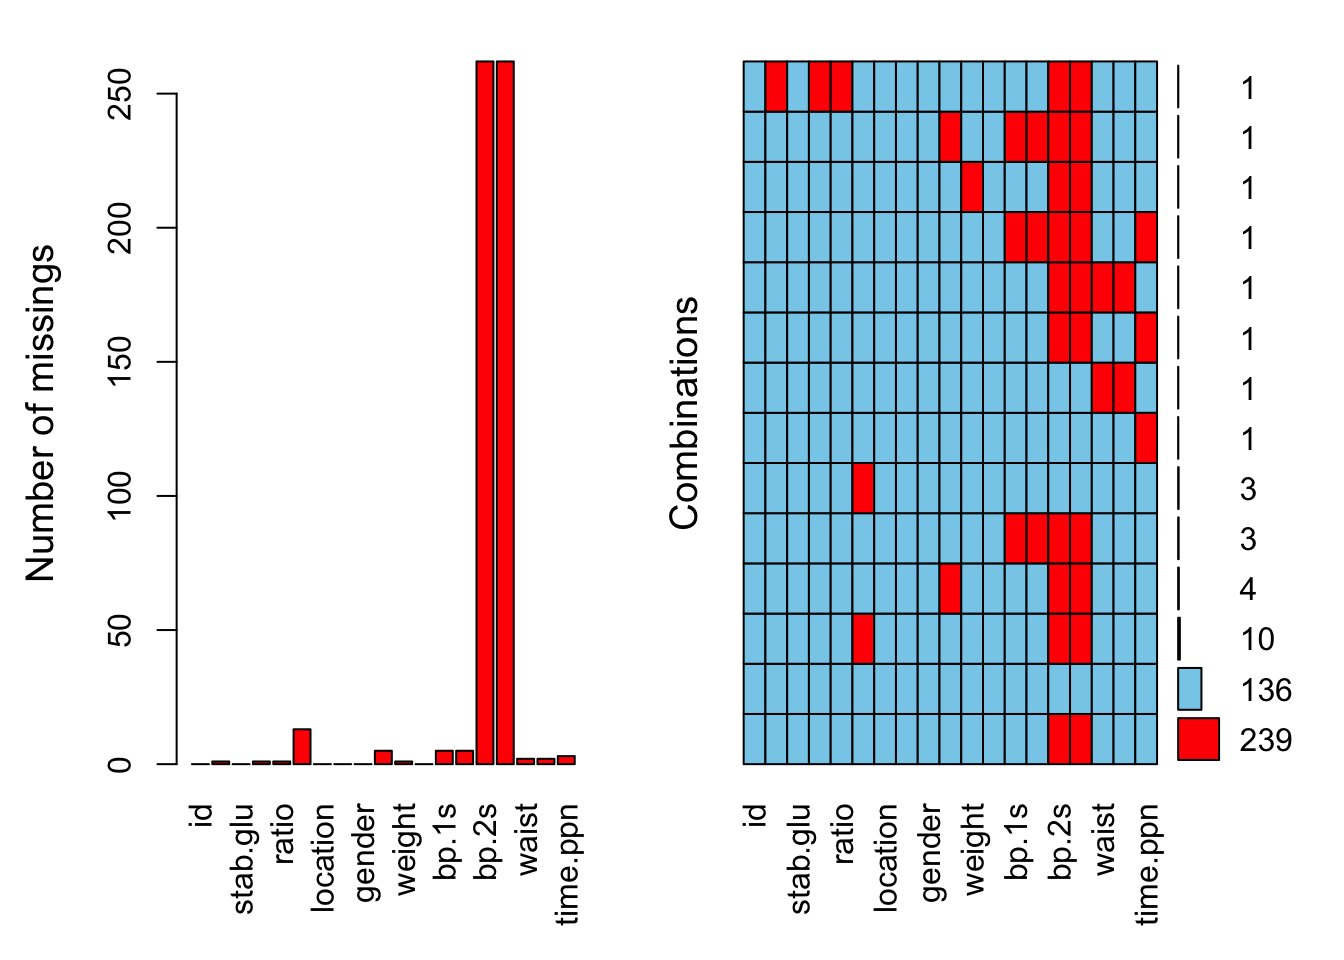
\includegraphics{main_files/figure-latex/unnamed-chunk-61-1.pdf} Siit on
näha, et kui me viskame välja 2 tulpa ja seejärel kõik read, mis
sisaldavad NA-sid, kaotame me umbes 20 rida 380-st, mis ei ole suur
kaotus.

Kui palju ridu, milles on 0 NA-d? Mitu \% kõikidest ridadest?

\begin{Shaded}
\begin{Highlighting}[]
\NormalTok{nrows <-}\StringTok{ }\KeywordTok{nrow}\NormalTok{(diabetes)}
\NormalTok{  ncomplete <-}\StringTok{ }\KeywordTok{sum}\NormalTok{(}\KeywordTok{complete.cases}\NormalTok{(diabetes))}
\NormalTok{  ncomplete }\CommentTok{#136}
\end{Highlighting}
\end{Shaded}

\begin{verbatim}
## [1] 136
\end{verbatim}

\begin{Shaded}
\begin{Highlighting}[]
\NormalTok{  ncomplete}\OperatorTok{/}\NormalTok{nrows }\CommentTok{#34%}
\end{Highlighting}
\end{Shaded}

\begin{verbatim}
## [1] 0.337469
\end{verbatim}

Mitu NA-d on igas tulbas?

\begin{Shaded}
\begin{Highlighting}[]
\KeywordTok{sapply}\NormalTok{(diabetes, }\ControlFlowTok{function}\NormalTok{(x) }\KeywordTok{sum}\NormalTok{(}\KeywordTok{is.na}\NormalTok{(x))) }
\end{Highlighting}
\end{Shaded}

\begin{verbatim}
##       id     chol stab.glu      hdl    ratio    glyhb location      age 
##        0        1        0        1        1       13        0        0 
##   gender   height   weight    frame    bp.1s    bp.1d    bp.2s    bp.2d 
##        0        5        1        0        5        5      262      262 
##    waist      hip time.ppn 
##        2        2        3
\end{verbatim}

Ploti NAd punasega igale tabeli reale ja tulbale mida tumedam halli toon
seda suurem number selle tulba kontekstis:

\begin{Shaded}
\begin{Highlighting}[]
\KeywordTok{matrixplot}\NormalTok{(diabetes) }
\end{Highlighting}
\end{Shaded}

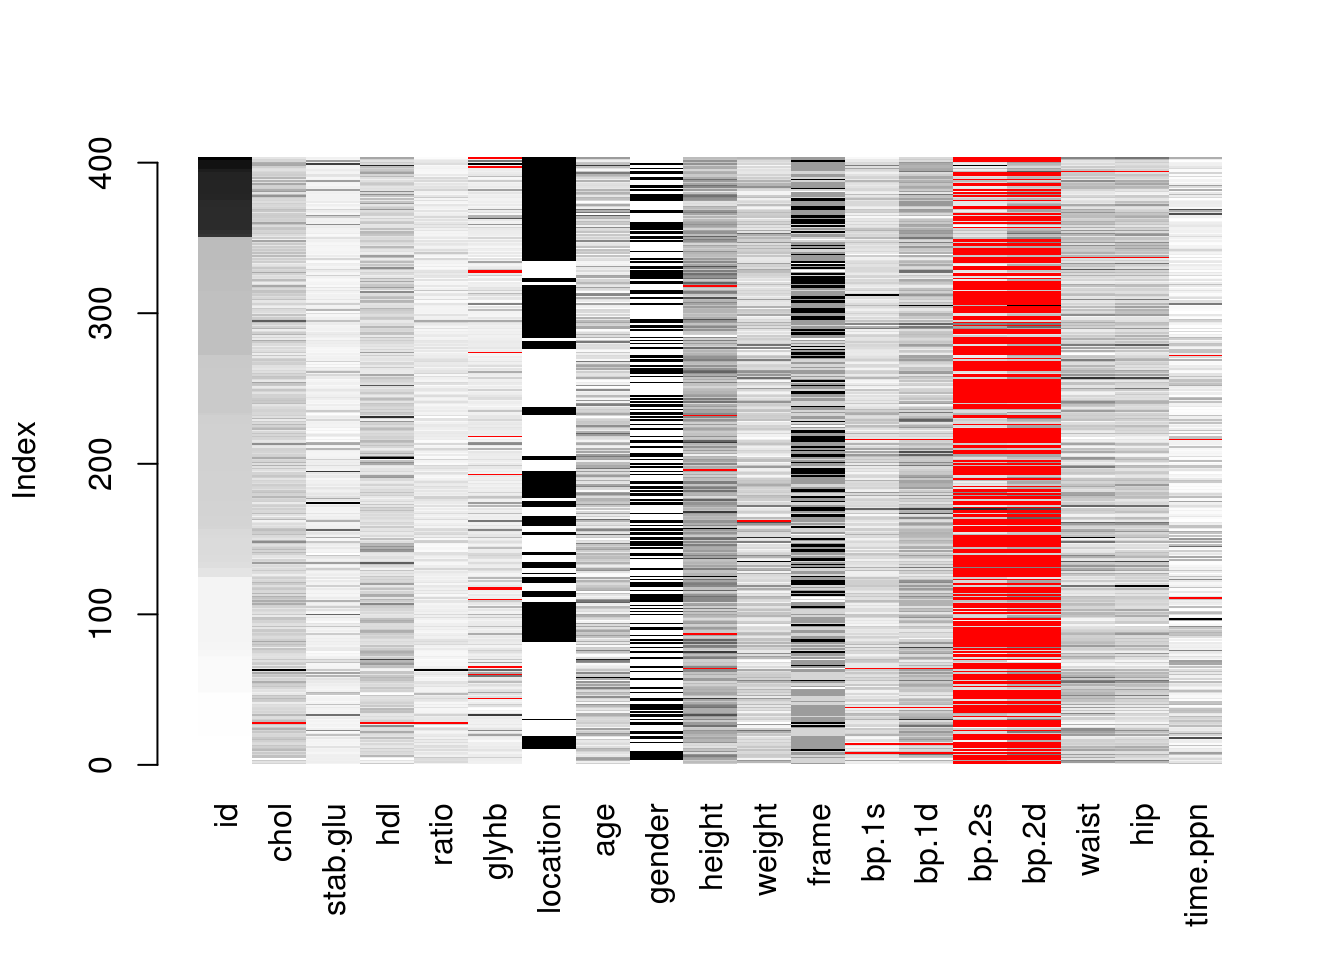
\includegraphics{main_files/figure-latex/unnamed-chunk-64-1.pdf}

Kuidas rekodeerida NA-d näiteks 0-ks:

\begin{Shaded}
\begin{Highlighting}[]
\NormalTok{dfs[}\KeywordTok{is.na}\NormalTok{(dfs)] <-}\StringTok{ }\DecValTok{0}
\NormalTok{dfs[}\KeywordTok{is.na}\NormalTok{(dfs)] <-}\StringTok{ "other"}
\NormalTok{dfs[dfs }\OperatorTok{==}\StringTok{ }\DecValTok{0}\NormalTok{] <-}\StringTok{ }\OtherTok{NA} \CommentTok{# teeb vastupidi 0-d NA-deks}
\end{Highlighting}
\end{Shaded}

Pane tähele, et NA tähistamine ei käi character vectorina vaid
dedikeeritud \texttt{is.na()} funktsiooniga.

\section{Matrix}\label{matrix}

Maatriks on 2-dimensionaalne vektor, sisaldab ainult ühte tüüpi andmeid
-- numbrid, stringid, faktorid. Tip: me saame sageli andmeraami
maatriksina kasutada kui me viskame sealt välja mitte-numbrilised
tulbad.

Aga saame ka andmeraame konverteerida otse maatriksiks (ja tagasi).

\begin{Shaded}
\begin{Highlighting}[]
\NormalTok{fruits <-}\StringTok{ }\KeywordTok{as.matrix}\NormalTok{(fruits)}
\KeywordTok{class}\NormalTok{(fruits)}
\end{Highlighting}
\end{Shaded}

\section{Indekseerimine}\label{indekseerimine}

Igale vektori, listi, andmeraami ja maatriksi elemendile vastab
unikaalne postiindeks, mille abil saame just selle elemendi unikaalselt
indentifitseerida, välja võtta ja töödelda.

Seega on indeksi mõte väga lühikese käsuga välja võtta R-i objektide
üksikuid elemente.

R-s algab indeksi numeratsioon 1-st (mitte 0-st, nagu näiteks Pythonis).

\subsection{Vektorid ja nende indeksid on
ühedimensionaalsed}\label{vektorid-ja-nende-indeksid-on-uhedimensionaalsed}

\begin{Shaded}
\begin{Highlighting}[]
\NormalTok{my_vector <-}\StringTok{ }\DecValTok{2}\OperatorTok{:}\DecValTok{5} 
\NormalTok{my_vector}
\end{Highlighting}
\end{Shaded}

\begin{verbatim}
## [1] 2 3 4 5
\end{verbatim}

\begin{Shaded}
\begin{Highlighting}[]
\NormalTok{my_vector[}\DecValTok{1}\NormalTok{] }\CommentTok{#1. element ehk number 2}
\end{Highlighting}
\end{Shaded}

\begin{verbatim}
## [1] 2
\end{verbatim}

\begin{Shaded}
\begin{Highlighting}[]
\NormalTok{my_vector[}\KeywordTok{c}\NormalTok{(}\DecValTok{1}\NormalTok{,}\DecValTok{3}\NormalTok{)] }\CommentTok{#1. ja 3. element }
\end{Highlighting}
\end{Shaded}

\begin{verbatim}
## [1] 2 4
\end{verbatim}

\begin{Shaded}
\begin{Highlighting}[]
\NormalTok{my_vector[}\OperatorTok{-}\DecValTok{1}\NormalTok{] }\CommentTok{#kõik elemendid, v.a. element number 1}
\end{Highlighting}
\end{Shaded}

\begin{verbatim}
## [1] 3 4 5
\end{verbatim}

\begin{Shaded}
\begin{Highlighting}[]
\NormalTok{my_vector[}\KeywordTok{c}\NormalTok{(}\OperatorTok{-}\DecValTok{1}\NormalTok{, }\OperatorTok{-}\DecValTok{3}\NormalTok{)] }\CommentTok{#kõik elemendid, v.a. element number 1 ja 3}
\end{Highlighting}
\end{Shaded}

\begin{verbatim}
## [1] 3 5
\end{verbatim}

\begin{Shaded}
\begin{Highlighting}[]
\NormalTok{my_vector[}\DecValTok{3}\OperatorTok{:}\DecValTok{5}\NormalTok{] }\CommentTok{#elemendid 3, 4 ja 5 (element 5 on määramata, seega NA)}
\end{Highlighting}
\end{Shaded}

\begin{verbatim}
## [1]  4  5 NA
\end{verbatim}

\begin{Shaded}
\begin{Highlighting}[]
\NormalTok{my_vector[}\OperatorTok{-}\NormalTok{(}\DecValTok{3}\OperatorTok{:}\KeywordTok{length}\NormalTok{(my_vector))] }\CommentTok{#1. ja 2. element}
\end{Highlighting}
\end{Shaded}

\begin{verbatim}
## [1] 2 3
\end{verbatim}

\subsection{Andmeraamid ja maatriksid on kahedimensionaalsed, nagu ka
nende
indeksid}\label{andmeraamid-ja-maatriksid-on-kahedimensionaalsed-nagu-ka-nende-indeksid}

\textbf{2D indeksi kuju on {[}rea\_indeks, veeru\_indeks{]}}.

\begin{Shaded}
\begin{Highlighting}[]
\NormalTok{dat <-}\StringTok{ }\KeywordTok{tibble}\NormalTok{(}\DataTypeTok{colA =} \KeywordTok{c}\NormalTok{(}\StringTok{"a"}\NormalTok{, }\StringTok{"b"}\NormalTok{, }\StringTok{"c"}\NormalTok{), }\DataTypeTok{colB =} \KeywordTok{c}\NormalTok{(}\DecValTok{1}\NormalTok{, }\DecValTok{2}\NormalTok{, }\DecValTok{3}\NormalTok{))}
\NormalTok{dat}
\CommentTok{# üks andmepunkt: 1 rida, 2. veerg}
\NormalTok{dat[}\DecValTok{1}\NormalTok{, }\DecValTok{2}\NormalTok{]}
\CommentTok{# 1. rida, kõik veerud}
\NormalTok{dat[}\DecValTok{1}\NormalTok{, ]}
\CommentTok{# 2. veerg, kõik read}
\NormalTok{dat[, }\DecValTok{2}\NormalTok{]}
\CommentTok{# kõik read peale 1.}
\NormalTok{dat[}\OperatorTok{-}\DecValTok{1}\NormalTok{, ]}
\CommentTok{# viskab välja 2. veeru}
\NormalTok{dat[, }\OperatorTok{-}\DecValTok{2}\NormalTok{]}
\CommentTok{# 2 andmepunkti: 2. rida, 1. ja 2. veerg}
\NormalTok{dat[}\DecValTok{2}\NormalTok{, }\DecValTok{1}\OperatorTok{:}\DecValTok{2}\NormalTok{]}
\CommentTok{# 2 andmepunkti: 2. rida, 3. ja 4. veerg}
\NormalTok{dat[}\DecValTok{2}\NormalTok{, }\KeywordTok{c}\NormalTok{(}\DecValTok{1}\NormalTok{, }\DecValTok{2}\NormalTok{)]}
\CommentTok{#viskab välja 1. ja 2. rea}
\NormalTok{dat[}\OperatorTok{-}\KeywordTok{c}\NormalTok{(}\DecValTok{1}\NormalTok{, }\DecValTok{2}\NormalTok{), ]}
\CommentTok{#veerg nimega colB, output on erandina vektor!}
\NormalTok{dat}\OperatorTok{$}\NormalTok{colB}
\end{Highlighting}
\end{Shaded}

Kui me indekseerimisega tibblest veeru ehk vektori välja võtame, on
output class: tibble. Kui me teeme sama data frame-st, siis on output
class: vector.

Nüüd veidi keerulisemad konstruktsioonid, mis võimaldavad tabeli ühe
kindla veeru väärtusi välja tõmmata teise veeru väärtuste järgi
filteerides. Püüdke sellest koodist aru saada, et te hiljem ära
tunneksite, kui midagi sellist vastu tuleb. Õnneks ei ole teil endil
vaja sellist koodi kirjutada, me õpetame teile varsti lihtsama filtri
meetodi.

\begin{Shaded}
\begin{Highlighting}[]
\NormalTok{dat <-}\StringTok{ }\KeywordTok{tibble}\NormalTok{(}\DataTypeTok{colA =} \KeywordTok{c}\NormalTok{(}\StringTok{"a"}\NormalTok{, }\StringTok{"b"}\NormalTok{, }\StringTok{"c"}\NormalTok{), }\DataTypeTok{colB =} \KeywordTok{c}\NormalTok{(}\DecValTok{1}\NormalTok{, }\DecValTok{2}\NormalTok{, }\DecValTok{3}\NormalTok{))}
\NormalTok{dat}\OperatorTok{$}\NormalTok{colB[dat}\OperatorTok{$}\NormalTok{colA }\OperatorTok{!=}\StringTok{ "a"}\NormalTok{ ] }\CommentTok{#jätab sisse kõik vektori colB väärtused, kus samas tabeli reas olev colA väärtus ei ole "a". output on vektor! }
\end{Highlighting}
\end{Shaded}

\begin{verbatim}
## [1] 2 3
\end{verbatim}

\begin{Shaded}
\begin{Highlighting}[]
\NormalTok{dat}\OperatorTok{$}\NormalTok{colA[dat}\OperatorTok{$}\NormalTok{colB }\OperatorTok{>}\StringTok{ }\DecValTok{1}\NormalTok{] }\CommentTok{#jätab sisse kõik vektori colA väärtused, kus samas tabeli reas olev colB väärtus >1. output on vektor. }
\end{Highlighting}
\end{Shaded}

\begin{verbatim}
## [1] "b" "c"
\end{verbatim}

\subsection{Listide indekseerimine}\label{listide-indekseerimine}

\textbf{Listi indekseerimisel kasutame kahte sorti nurksulge, ``{[}
{]}'' ja ``{[}{[} {]}{]}'', mis töötavad erinevalt}.

Kui listi vaadata nagu objektide vanglat, siis kaksiksulgude
\texttt{{[}{[}\ {]}{]}} abil on võimalik üksikuid objekte vanglast välja
päästa nii, et taastub nende algne kuju ehk class. Seevastu üksiksulud
\texttt{{[}\ {]}} tekitavad uue listi, kus on säilinud osad algse listi
elemendid, ehk uue vangla vähemate vangidega.

\begin{quote}
Kaksiksulud ``{[}{[} {]}{]}'' päästavad listist välja ühe elemendi ja
taastavad selle algse class-i (data.frame, vektor, list jms). Üksiksulud
``{[} {]}'' võtavad algsest listist välja teie poolt valitud elemendid
aga jätavad uue objekti ikka listi kujule.
\end{quote}

\begin{Shaded}
\begin{Highlighting}[]
\NormalTok{my_list <-}\StringTok{ }\KeywordTok{list}\NormalTok{(}\DataTypeTok{a =} \KeywordTok{tibble}\NormalTok{(}\DataTypeTok{colA =} \KeywordTok{c}\NormalTok{(}\StringTok{"A"}\NormalTok{, }\StringTok{"B"}\NormalTok{), }\DataTypeTok{colB =} \KeywordTok{c}\NormalTok{(}\DecValTok{1}\NormalTok{, }\DecValTok{2}\NormalTok{)), }\DataTypeTok{b =} \KeywordTok{c}\NormalTok{(}\DecValTok{1}\NormalTok{, }\OtherTok{NA}\NormalTok{, }\StringTok{"s"}\NormalTok{))}
\NormalTok{## this list has two elements, a data frame called "a" and a character vector called "b".}
\KeywordTok{str}\NormalTok{(my_list)}
\end{Highlighting}
\end{Shaded}

\begin{verbatim}
## List of 2
##  $ a:Classes 'tbl_df', 'tbl' and 'data.frame':   2 obs. of  2 variables:
##   ..$ colA: chr [1:2] "A" "B"
##   ..$ colB: num [1:2] 1 2
##  $ b: chr [1:3] "1" NA "s"
\end{verbatim}

Tõmbame listist välja tibble:

\begin{Shaded}
\begin{Highlighting}[]
\NormalTok{my_tibble <-}\StringTok{ }\NormalTok{my_list[[}\DecValTok{1}\NormalTok{]]}
\NormalTok{my_tibble}
\end{Highlighting}
\end{Shaded}

\begin{verbatim}
## # A tibble: 2 x 2
##    colA  colB
##   <chr> <dbl>
## 1     A     1
## 2     B     2
\end{verbatim}

See ei ole enam list.

Nüüd võtame üksiksuluga listist välja 1. elemendi, mis on tibble, aga
output ei ole mitte tibble, vaid ikka list. Seekord ühe elemendiga, mis
on tibble.

\begin{Shaded}
\begin{Highlighting}[]
\NormalTok{aa <-}\StringTok{ }\NormalTok{my_list[}\DecValTok{1}\NormalTok{]}
\KeywordTok{str}\NormalTok{(aa)}
\end{Highlighting}
\end{Shaded}

\begin{verbatim}
## List of 1
##  $ a:Classes 'tbl_df', 'tbl' and 'data.frame':   2 obs. of  2 variables:
##   ..$ colA: chr [1:2] "A" "B"
##   ..$ colB: num [1:2] 1 2
\end{verbatim}

\begin{Shaded}
\begin{Highlighting}[]
\NormalTok{aa1 <-}\StringTok{ }\NormalTok{my_list}\OperatorTok{$}\NormalTok{a[}\DecValTok{2}\NormalTok{,] }\CommentTok{#class is df}
\NormalTok{aa1}
\end{Highlighting}
\end{Shaded}

\begin{verbatim}
## # A tibble: 1 x 2
##    colA  colB
##   <chr> <dbl>
## 1     B     2
\end{verbatim}

\begin{Shaded}
\begin{Highlighting}[]
\NormalTok{aa3 <-}\StringTok{ }\NormalTok{my_list[[}\DecValTok{1}\NormalTok{]][}\DecValTok{1}\NormalTok{,]}
\NormalTok{aa3}
\end{Highlighting}
\end{Shaded}

\begin{verbatim}
## # A tibble: 1 x 2
##    colA  colB
##   <chr> <dbl>
## 1     A     1
\end{verbatim}

Kõigepealt läksime kaksiksulgudega listi taseme võrra sisse ja võtsime
välja objekti my\_list 1. elemendi, tema algses tibble formaadis,
(indeksi 1. dimensioon). Seejärel korjame sealt välja 1. rea, tibble
formaati muutmata ja seega üksiksulgudes (indeksi 2. ja 3. dimensioon).

Pane tähele, et \texttt{{[}{[}\ {]}{]}} lubab ainult ühe elemendi
korraga listist välja päästa.

\chapter{Regular expression ja find \& replace}\label{regex}

Regular expression annab võimaluse lühidalt kirjeldada mitte-üheseid
otsinguparameetreid.

\begin{quote}
regular expression on string, mis kirjeldab mitut stringi
\end{quote}

A
\href{https://stat.ethz.ch/R-manual/R-devel/library/base/html/regex.html}{regular
expression}
\href{https://stat.ethz.ch/R-manual/R-devel/library/base/html/regex.html}{Regular
Expressions as used in R}

\begin{itemize}
\tightlist
\item
  Most characters, including all letters and digits, are regular
  expressions that match themselves.
\item
  \texttt{.} matches any single character.
\item
  You can refer also to a character class, which is a list of characters
  enclosed between \texttt{{[}} and \texttt{{]}}, e.g.
  \texttt{{[}{[}:alnum:{]}{]}} is same as \texttt{{[}A-z0-9{]}}.
\item
  Most common character classes:
\item
  \texttt{{[}:alnum:{]}} includes alphanumerics (\texttt{{[}:alpha:{]}}
  and \texttt{{[}:digit:{]}});
\item
  \texttt{{[}:alpha:{]}}, includes alphabetic characters
  (\texttt{{[}:upper:{]}} and \texttt{{[}:lower:{]}} case);
\item
  \texttt{{[}:punct:{]}} includes punctuation characters ! " \# \$ \% \&
  ' ( ) * + , - . / : ; \textless{} = \textgreater{} ? @ {[} ~{]} \^{}
  \_ ` ` \{ \textbar{} \} \textasciitilde{}.;
\item
  \texttt{{[}:blank:{]}} includes space and tab; etc.
\item
  The metacharacters in regular expressions are
  \texttt{.\ \textbackslash{}\ \textbar{}\ (\ )\ {[}\ \{\ \^{}\ \$\ *\ +\ ?},
  whether these have a special meaning depends on the context. When
  matching a metacharacter as a regular character, precede it with a
  double backslash \texttt{\textbackslash{}\textbackslash{}}.
\item
  Repetition quantifiers put after regex specify how many times regex is
  matched: \texttt{?}, optional, at most once; \texttt{*}, zero or more
  times; \texttt{+}, one or more times; \texttt{\{n\}}, n times;
  \texttt{\{n,\}}, n or more times; \texttt{\{n,m\}}, n to m times.
\item
  \^{} anchors the regular expression to the start of the string.
\item
  \$ anchors the the regular expression to end of the string.
\end{itemize}

\subsection{Common operations with regular
expressions}\label{common-operations-with-regular-expressions}

\begin{itemize}
\tightlist
\item
  Locate a pattern match (positions)
\item
  Extract a matched pattern
\item
  Identify a match to a pattern
\item
  Replace a matched pattern
\end{itemize}

\subsection{Find and replace}\label{find-and-replace}

\begin{Shaded}
\begin{Highlighting}[]
\KeywordTok{library}\NormalTok{(stringr)}
\NormalTok{x<-}\StringTok{ }\KeywordTok{c}\NormalTok{(}\StringTok{"apple"}\NormalTok{, }\StringTok{"ananas"}\NormalTok{, }\StringTok{"banana"}\NormalTok{)}

\CommentTok{#replaces all a-s at the beginning of strings with e-s}
\KeywordTok{str_replace}\NormalTok{(x, }\StringTok{"^a"}\NormalTok{, }\StringTok{"e"}\NormalTok{) }
\end{Highlighting}
\end{Shaded}

\begin{verbatim}
## [1] "epple"  "enanas" "banana"
\end{verbatim}

\begin{Shaded}
\begin{Highlighting}[]
\CommentTok{# str_replace only replaces at the first occurence at each string}
\KeywordTok{str_replace}\NormalTok{(x, }\StringTok{"a"}\NormalTok{, }\StringTok{"e"}\NormalTok{) }
\end{Highlighting}
\end{Shaded}

\begin{verbatim}
## [1] "epple"  "enanas" "benana"
\end{verbatim}

\begin{Shaded}
\begin{Highlighting}[]
\CommentTok{#str_replace_all replaces all a-s anywhere in the strings}
\KeywordTok{str_replace_all}\NormalTok{(x, }\StringTok{"a"}\NormalTok{, }\StringTok{"e"}\NormalTok{) }
\end{Highlighting}
\end{Shaded}

\begin{verbatim}
## [1] "epple"  "enenes" "benene"
\end{verbatim}

\begin{Shaded}
\begin{Highlighting}[]
\CommentTok{#replaces a and the following character at the end of string with nothing (i.e. deletes 2 chars)}
\KeywordTok{str_replace}\NormalTok{(x, }\StringTok{"a.$"}\NormalTok{, }\StringTok{""}\NormalTok{)}
\end{Highlighting}
\end{Shaded}

\begin{verbatim}
## [1] "apple"  "anan"   "banana"
\end{verbatim}

\begin{Shaded}
\begin{Highlighting}[]
\CommentTok{#replaces a-s or s-s at the end of string with e-s}
\KeywordTok{str_replace}\NormalTok{(x, }\StringTok{"(a|s)$"}\NormalTok{, }\StringTok{"e"}\NormalTok{)}
\end{Highlighting}
\end{Shaded}

\begin{verbatim}
## [1] "apple"  "ananae" "banane"
\end{verbatim}

\begin{Shaded}
\begin{Highlighting}[]
\CommentTok{#replaces a-s or s-s anywhere in the string with e-s}
\KeywordTok{str_replace_all}\NormalTok{(x, }\StringTok{"a|s"}\NormalTok{, }\StringTok{"e"}\NormalTok{)}
\end{Highlighting}
\end{Shaded}

\begin{verbatim}
## [1] "epple"  "enenee" "benene"
\end{verbatim}

\begin{Shaded}
\begin{Highlighting}[]
\CommentTok{#remove all numbers. }
\NormalTok{y<-}\KeywordTok{c}\NormalTok{(}\StringTok{"as1"}\NormalTok{, }\StringTok{"2we3w"}\NormalTok{, }\StringTok{"3e"}\NormalTok{)}
\KeywordTok{str_replace_all}\NormalTok{(y, }\StringTok{"}\CharTok{\textbackslash{}\textbackslash{}}\StringTok{d"}\NormalTok{, }\StringTok{""}\NormalTok{) }
\end{Highlighting}
\end{Shaded}

\begin{verbatim}
## [1] "as"  "wew" "e"
\end{verbatim}

\begin{Shaded}
\begin{Highlighting}[]
\CommentTok{#remove everything, except numbers. }
\KeywordTok{str_replace_all}\NormalTok{(y, }\StringTok{"[A-Za-z_]"}\NormalTok{, }\StringTok{""}\NormalTok{) }
\end{Highlighting}
\end{Shaded}

\begin{verbatim}
## [1] "1"  "23" "3"
\end{verbatim}

\begin{Shaded}
\begin{Highlighting}[]
\NormalTok{x<-}\StringTok{ }\KeywordTok{c}\NormalTok{(}\StringTok{"apple"}\NormalTok{, }\StringTok{"apple pie"}\NormalTok{)}
\KeywordTok{str_replace_all}\NormalTok{(x, }\StringTok{"^apple$"}\NormalTok{,}\StringTok{"m"}\NormalTok{) }\CommentTok{#To force to only match a complete string:}
\end{Highlighting}
\end{Shaded}

\begin{verbatim}
## [1] "m"         "apple pie"
\end{verbatim}

\begin{Shaded}
\begin{Highlighting}[]
\KeywordTok{str_replace_all}\NormalTok{(x, }\StringTok{"}\CharTok{\textbackslash{}\textbackslash{}}\StringTok{s"}\NormalTok{,}\StringTok{"_"}\NormalTok{) }\CommentTok{#space to _}
\end{Highlighting}
\end{Shaded}

\begin{verbatim}
## [1] "apple"     "apple_pie"
\end{verbatim}

\begin{Shaded}
\begin{Highlighting}[]
\KeywordTok{str_replace_all}\NormalTok{(x, }\StringTok{"[apl]"}\NormalTok{,}\StringTok{"_"}\NormalTok{) }\CommentTok{#a or p or l to _}
\end{Highlighting}
\end{Shaded}

\begin{verbatim}
## [1] "____e"     "____e _ie"
\end{verbatim}

\begin{Shaded}
\begin{Highlighting}[]
\KeywordTok{str_replace_all}\NormalTok{(x, }\StringTok{"[ap|p.e]"}\NormalTok{,}\StringTok{"_"}\NormalTok{) }\CommentTok{# ap or p.e to _}
\end{Highlighting}
\end{Shaded}

\begin{verbatim}
## [1] "___l_"     "___l_ _i_"
\end{verbatim}

\textbf{patterns that match more than one character:}

\begin{Shaded}
\begin{Highlighting}[]
\NormalTok{. (dot)}\OperatorTok{:}\StringTok{ }\NormalTok{any character apart from a newline.}

\NormalTok{\textbackslash{}\textbackslash{}d}\OperatorTok{:}\StringTok{ }\NormalTok{any digit.}

\NormalTok{\textbackslash{}\textbackslash{}s}\OperatorTok{:}\StringTok{ }\NormalTok{any }\KeywordTok{whitespace}\NormalTok{ (space, tab, newline).}

\NormalTok{\textbackslash{}[abc]}\OperatorTok{:}\StringTok{ }\NormalTok{match a, b, or c.}

\NormalTok{\textbackslash{}[}\OperatorTok{!}\NormalTok{abc]}\OperatorTok{:}\StringTok{ }\NormalTok{match anything except a, b, or c.}

\NormalTok{To create a regular expression containing \textbackslash{}d or \textbackslash{}s, you???ll need to escape the \textbackslash{} }\ControlFlowTok{for}\NormalTok{ the string, so you will type }\StringTok{"}\CharTok{\textbackslash{}\textbackslash{}\textbackslash{}\textbackslash{}}\StringTok{d"}\NormalTok{ or }\StringTok{"}\CharTok{\textbackslash{}\textbackslash{}\textbackslash{}\textbackslash{}}\StringTok{s"}\NormalTok{.}

\NormalTok{abc}\OperatorTok{|}\NormalTok{d..f will match either }\StringTok{"abc"}\NormalTok{, or }\StringTok{"deaf"}\NormalTok{. }
\end{Highlighting}
\end{Shaded}

\chapter{Funktsioonid on R keele verbid}\label{funs}

Kasutaja ütleb nii täpselt kui oskab, mida ta tahab ja R-s elab kratt,
kes püüab ära arvata, mida on vaja teha. Vahest teeb kah. Vahest isegi
seda, mida kasutaja tahtis. Mõni arvab, et R-i puudus on veateadete
puudumine või krüptilised veateated. Sama kehtib ka R-i helpi kohta.
Seega tasub alati kontrollida, kas R ikka tegi seda, mida sina talle
enda arust ette kirjutasid.

Paljudel juhtudel ütleb (hea) funktsiooni nimi mida see teeb:

\begin{Shaded}
\begin{Highlighting}[]
\CommentTok{# create two test vectors}
\NormalTok{x <-}\StringTok{ }\KeywordTok{c}\NormalTok{(}\DecValTok{6}\NormalTok{, }\DecValTok{3}\NormalTok{, }\DecValTok{3}\NormalTok{, }\DecValTok{4}\NormalTok{, }\DecValTok{5}\NormalTok{)}
\NormalTok{y <-}\StringTok{ }\KeywordTok{c}\NormalTok{(}\DecValTok{1}\NormalTok{, }\DecValTok{3}\NormalTok{, }\DecValTok{4}\NormalTok{, }\DecValTok{2}\NormalTok{, }\DecValTok{7}\NormalTok{)}
\end{Highlighting}
\end{Shaded}

\begin{Shaded}
\begin{Highlighting}[]
\CommentTok{# calculate correlation}
\KeywordTok{cor}\NormalTok{(x, y)}
\end{Highlighting}
\end{Shaded}

\begin{verbatim}
## [1] -0.1166019
\end{verbatim}

\begin{Shaded}
\begin{Highlighting}[]
\CommentTok{# calculate sum}
\KeywordTok{sum}\NormalTok{(x)}
\end{Highlighting}
\end{Shaded}

\begin{verbatim}
## [1] 21
\end{verbatim}

\begin{Shaded}
\begin{Highlighting}[]
\CommentTok{# calculate sum of two vectors}
\KeywordTok{sum}\NormalTok{(x, y)}
\end{Highlighting}
\end{Shaded}

\begin{verbatim}
## [1] 38
\end{verbatim}

\begin{Shaded}
\begin{Highlighting}[]
\CommentTok{# calculate average}
\KeywordTok{mean}\NormalTok{(x)}
\end{Highlighting}
\end{Shaded}

\begin{verbatim}
## [1] 4.2
\end{verbatim}

\begin{Shaded}
\begin{Highlighting}[]
\CommentTok{# calculate median}
\KeywordTok{median}\NormalTok{(x)}
\end{Highlighting}
\end{Shaded}

\begin{verbatim}
## [1] 4
\end{verbatim}

\begin{Shaded}
\begin{Highlighting}[]
\CommentTok{# calculate standard deviation}
\KeywordTok{sd}\NormalTok{(x)}
\end{Highlighting}
\end{Shaded}

\begin{verbatim}
## [1] 1.30384
\end{verbatim}

\begin{Shaded}
\begin{Highlighting}[]
\CommentTok{# return quantiles}
\KeywordTok{quantile}\NormalTok{(x)}
\end{Highlighting}
\end{Shaded}

\begin{verbatim}
##   0%  25%  50%  75% 100% 
##    3    3    4    5    6
\end{verbatim}

\begin{Shaded}
\begin{Highlighting}[]
\CommentTok{# return maximum value}
\KeywordTok{max}\NormalTok{(x)}
\end{Highlighting}
\end{Shaded}

\begin{verbatim}
## [1] 6
\end{verbatim}

\begin{Shaded}
\begin{Highlighting}[]
\CommentTok{# return minimum value}
\KeywordTok{min}\NormalTok{(x)}
\end{Highlighting}
\end{Shaded}

\begin{verbatim}
## [1] 3
\end{verbatim}

R-is teevad asju programmikesed, mida kutsutakse
\textbf{funktsioonideks}. Te võite mõelda funktsioonist nagu verbist.
Näiteks funktsiooni \texttt{sum()} korral loe: ``võta summa''. Iga
funktsiooni nime järel on sulud. Nende sulgude sees asuvad selle
funktsiooni \textbf{argumendid}. Argumendid määravad ära funktsiooni
käitumise. Et näha, millised argumendid on funktsiooni käivitamiseks
vajalikud ja milliseid on üldse võimalik seadistada, kasuta `help'
käsku.

\begin{Shaded}
\begin{Highlighting}[]
\NormalTok{?sum}
\end{Highlighting}
\end{Shaded}

Help paneelis paremal all ilmub nüüd selle funktsiooni R
dokumentatsioon. Vaata seal peatükki Usage:
\texttt{sum(...,\ na.rm\ =\ FALSE)} ja edasi peatükki Arguments, mis
ütleb, et \texttt{...} (ellipsis) tähistab vektoreid.

\begin{verbatim}
sum {base}  R Documentation 
Sum of Vector Elements

Description:

sum returns the sum of all the values present in its arguments.

Usage

sum(..., na.rm = FALSE)

Arguments

... - numeric or complex or logical vectors.

na.rm   - logical. Should missing values (including NaN) be removed?
\end{verbatim}

Seega võtab funktsioon \texttt{sum()} kaks argumenti: vektori arvudest
(või loogilise vektori, mis koosneb TRUE ja FALSE määrangutest), ning
``na.rm'' argumendi, millele saab anda väärtuseks kas, TRUE või FALSE.
Usage ütleb ka, et vaikimisi on \texttt{na.rm\ =\ FALSE}, mis tähendab,
et sellele argumendile on antud vaikeväärtus -- kui me seda ise ei
muuda, siis jäävad NA-d arvutusse sisse. Kuna NA tähendab ``tundmatu
arv'' siis iga tehe NA-dega annab vastuseks ``tundmatu arv'' ehk NA
(tundmatu arv + 2 = tundmatu arv). Seega NA tulemus annab märku, et teie
andmetes võib olla midagi valesti.

\begin{Shaded}
\begin{Highlighting}[]
\NormalTok{## moodustame vektori}
\NormalTok{apples <-}\StringTok{ }\KeywordTok{c}\NormalTok{(}\DecValTok{1}\NormalTok{, }\DecValTok{34}\NormalTok{, }\DecValTok{43}\NormalTok{, }\OtherTok{NA}\NormalTok{)}
\NormalTok{## arvutame summa}
\KeywordTok{sum}\NormalTok{(apples, }\DataTypeTok{na.rm =} \OtherTok{TRUE}\NormalTok{)}
\end{Highlighting}
\end{Shaded}

\begin{verbatim}
## [1] 78
\end{verbatim}

Niimoodi saab arvutada summat vektorile nimega ``apples''.

Sisestades R käsureale funktsiooni ilma selle sulgudeta saab masinast
selle funktsiooni koodi. Näiteks:

\begin{Shaded}
\begin{Highlighting}[]
\NormalTok{sum}
\end{Highlighting}
\end{Shaded}

\begin{verbatim}
## function (..., na.rm = FALSE)  .Primitive("sum")
\end{verbatim}

Tulemus näitab, et \texttt{sum()} on \texttt{Primitive} funktsioon, mis
põhimõtteliselt tähendab, et ta põhineb C koodil ja ei kasuta R koodi.

\section{Kirjutame R funktsiooni}\label{kirjutame-r-funktsiooni}

Võib ju väita, et funktsiooni ainus mõte on peita teie eest korduvad
vajalikud koodiread kood funktsiooni nime taha. Põhjus, miks R-s on
funktsioonid, on korduse vähendamine, koodi loetavaks muutmine ja seega
ka ruumi kokkuhoid. Koodi funktsioonidena kasutamine suurendab
analüüside reprodutseeritavust, kuna funktsioonis olev kood pärineb
ühest allikast, mitte ei ole paljude koopiatena igal pool laiali. See
muudab pikad koodilõigud hõlpsalt taaskasutatavaks sest lihtsam on
kirjutada lühike funktsiooni nimi ja sisestada selle funktsiooni
argumendid. Koodi funktsioonidesse kokku surumine vähendab võimalusi
lollideks vigadeks, mida te võite teha pikkade koodijuppidega
manipuleerides. Seega tasub teil õppida ka oma korduvaid koodiridu
funktsioonidena vormistama.

Kõige pealt kirjutame natuke koodi.

\begin{Shaded}
\begin{Highlighting}[]
\CommentTok{# two apples}
\NormalTok{apples <-}\StringTok{ }\DecValTok{2}
\CommentTok{# three oranges}
\NormalTok{oranges <-}\StringTok{ }\DecValTok{3} 
\CommentTok{# parentheses around expression assigning result to an object }
\CommentTok{# ensure that result is also printed to R console}
\NormalTok{(inventory <-}\StringTok{ }\NormalTok{apples }\OperatorTok{+}\StringTok{ }\NormalTok{oranges)}
\end{Highlighting}
\end{Shaded}

\begin{verbatim}
## [1] 5
\end{verbatim}

Ja nüüd pakendame selle tehte funktsiooni \texttt{add2()}. Funktsiooni
defineerimiseks kasutame järgmist r ekspressiooni
\texttt{function(\ arglist\ )\ expr}, kus ``arglist'' on tühi või ühe
või rohkema nimega argumenti kujul \texttt{name=expression}; ``expr'' on
R-i ekspressioon st. kood mida see funktsioon käivitab. Funktsiooni
viimane evlueeritav koodirida on see, mis tuleb välja selle funktsiooni
outputina.

All toodud näites on selleks \texttt{x\ +\ y} tehte vastus.

\begin{Shaded}
\begin{Highlighting}[]
\NormalTok{add2 <-}\StringTok{ }\ControlFlowTok{function}\NormalTok{(x, y) \{}
\NormalTok{    x }\OperatorTok{+}\StringTok{ }\NormalTok{y}
\NormalTok{\}}
\end{Highlighting}
\end{Shaded}

Seda koodi jooksutades näeme, et meie funktsioon ilmub R-i Environmenti,
kuhu tekib Functions lahter. Seal on näha ka selle funktsiooni kaks
argumenti, apples ja oranges.

Antud funktsiooni käivitamine annab veateate, sest funktsiooni
argumentidel pole väärtusi:

\begin{Shaded}
\begin{Highlighting}[]
\NormalTok{## run function in failsafe mode}
\NormalTok{inventory <-}\StringTok{ }\KeywordTok{try}\NormalTok{(}\KeywordTok{add2}\NormalTok{())}
\NormalTok{## when function fails, error message is returned}
\KeywordTok{class}\NormalTok{(inventory)}
\end{Highlighting}
\end{Shaded}

\begin{verbatim}
## [1] "try-error"
\end{verbatim}

\begin{Shaded}
\begin{Highlighting}[]
\NormalTok{## print error message}
\KeywordTok{cat}\NormalTok{(inventory)}
\end{Highlighting}
\end{Shaded}

\begin{verbatim}
## Error in add2() : argument "x" is missing, with no default
\end{verbatim}

Andes funktsiooni argumentidele väärtused, saab väljundi:

\begin{Shaded}
\begin{Highlighting}[]
\NormalTok{## run function with proper arguments}
\NormalTok{inventory <-}\StringTok{ }\KeywordTok{add2}\NormalTok{(}\DataTypeTok{x =}\NormalTok{ apples, }\DataTypeTok{y =}\NormalTok{ oranges)}
\NormalTok{## numeric vector is returned}
\KeywordTok{class}\NormalTok{(inventory)}
\end{Highlighting}
\end{Shaded}

\begin{verbatim}
## [1] "numeric"
\end{verbatim}

\begin{Shaded}
\begin{Highlighting}[]
\NormalTok{## result}
\NormalTok{inventory}
\end{Highlighting}
\end{Shaded}

\begin{verbatim}
## [1] 5
\end{verbatim}

\textbf{Nüüd midagi kasulikumat!}

Funktsioon standrardvea arvutamiseks (baas R-s sellist funktsiooni ei
ole): \texttt{sd()} funktsioon arvutab standardhälbe. Sellel on kaks
argumenti: x and na.rm. Me teame, et SEM=SD/sqrt(N) kus N = length(x)

\begin{Shaded}
\begin{Highlighting}[]
\NormalTok{calc_sem <-}\StringTok{ }\ControlFlowTok{function}\NormalTok{(x) \{}
\NormalTok{  stdev <-}\StringTok{ }\KeywordTok{sd}\NormalTok{(x)}
\NormalTok{  n <-}\StringTok{ }\KeywordTok{length}\NormalTok{(x)}
\NormalTok{  stdev }\OperatorTok{/}\StringTok{ }\KeywordTok{sqrt}\NormalTok{(n)}
\NormalTok{\}}
\end{Highlighting}
\end{Shaded}

x hoiab lihtsalt kohta andmetele, mida me tahame sinna funktsiooni
suunata. \texttt{sd()}, \texttt{sqrt()} ja \texttt{length()} on
olemasolevad baas R funktsioonid, mille me oma funktsiooni hõlmame.

\begin{Shaded}
\begin{Highlighting}[]
\NormalTok{## create numeric vector}
\NormalTok{numbers <-}\StringTok{ }\KeywordTok{c}\NormalTok{(}\DecValTok{2}\NormalTok{, }\FloatTok{3.4}\NormalTok{, }\DecValTok{54}\NormalTok{, }\OtherTok{NA}\NormalTok{, }\DecValTok{3}\NormalTok{)}
\KeywordTok{calc_sem}\NormalTok{(numbers)}
\end{Highlighting}
\end{Shaded}

\begin{verbatim}
## [1] NA
\end{verbatim}

No jah, kui meil on andmetes tundmatu arv (\texttt{NA}) siis on ka
tulemuseks tundmatu arv.

Sellisel juhul tuleb NA väärtused vektorist enne selle funktsiooni
kasutamist välja visata:

\begin{Shaded}
\begin{Highlighting}[]
\NormalTok{numbers_filtered <-}\StringTok{ }\KeywordTok{na.omit}\NormalTok{(numbers)}
\KeywordTok{calc_sem}\NormalTok{(numbers_filtered)}
\end{Highlighting}
\end{Shaded}

\begin{verbatim}
## [1] 12.80338
\end{verbatim}

On ka võimalus funktsiooni sisse kirjutada \textbf{NA väärtuste
käsitlemine}. Näiteks, üks võimalus on \textbf{anda viga} ja funktsioon
katkestada, et kasutaja saaks ise ühemõtteliselt oma andmetest NA
väärtused eemaldada. Teine võimalus on funktsioonis \textbf{NA-d
vaikimisi eemaldada} ja anda selle kohta näiteks teade.

NA-de vaikimisi eemaldamiseks on hetkel mitu võimalust, kasutame
kõigepealt nö. valet lahendust:

\begin{Shaded}
\begin{Highlighting}[]
\NormalTok{calc_sem <-}\StringTok{ }\ControlFlowTok{function}\NormalTok{(x) \{}
\NormalTok{  ## kasutame sd funktsiooni argumenti na.rm}
\NormalTok{  stdev <-}\StringTok{ }\KeywordTok{sd}\NormalTok{(x, }\DataTypeTok{na.rm =} \OtherTok{TRUE}\NormalTok{)}
\NormalTok{  n <-}\StringTok{ }\KeywordTok{length}\NormalTok{(x)}
\NormalTok{  stdev }\OperatorTok{/}\StringTok{ }\KeywordTok{sqrt}\NormalTok{(n)}
\NormalTok{\}}

\KeywordTok{calc_sem}\NormalTok{(numbers)}
\end{Highlighting}
\end{Shaded}

\begin{verbatim}
## [1] 11.4517
\end{verbatim}

See annab meile vale tulemuse sest \texttt{na.rm\ =\ TRUE} viskab küll
NA-d välja meie vektorist aga jätab vektori pikkuse muutmata
(\texttt{length(x)} rida).

Teeme uue versiooni oma funktsioonist, mis viskab vaikimisi välja
puuduvad väärtused, kui need on olemas ja annab siis ka selle kohta
hoiatuse.

\begin{Shaded}
\begin{Highlighting}[]
\NormalTok{## x on numbriline vektor}
\NormalTok{calc_sem <-}\StringTok{ }\ControlFlowTok{function}\NormalTok{(x) \{}
  
\NormalTok{  ## viskame NA väärtused vektorist välja}
\NormalTok{  x <-}\StringTok{ }\KeywordTok{na.omit}\NormalTok{(x)}
  
\NormalTok{  ## kui vektoris on NA väärtusi, siis hoiatame kasutajat}
  \ControlFlowTok{if}\NormalTok{(}\KeywordTok{inherits}\NormalTok{(}\KeywordTok{na.action}\NormalTok{(x), }\StringTok{"omit"}\NormalTok{)) \{}
    \KeywordTok{warning}\NormalTok{(}\StringTok{"Removed NAs from vector.}\CharTok{\textbackslash{}n}\StringTok{"}\NormalTok{)}
\NormalTok{  \}}
  
\NormalTok{  ## arvutame standardvea kasutades filtreeritud vektorit}
\NormalTok{  stdev <-}\StringTok{ }\KeywordTok{sd}\NormalTok{(x)}
\NormalTok{  n <-}\StringTok{ }\KeywordTok{length}\NormalTok{(x)}
\NormalTok{  stdev }\OperatorTok{/}\StringTok{ }\KeywordTok{sqrt}\NormalTok{(n)}
\NormalTok{\}}

\KeywordTok{calc_sem}\NormalTok{(numbers)}
\end{Highlighting}
\end{Shaded}

\begin{verbatim}
## Warning in calc_sem(numbers): Removed NAs from vector.
\end{verbatim}

\begin{verbatim}
## [1] 12.80338
\end{verbatim}

\begin{Shaded}
\begin{Highlighting}[]
\KeywordTok{length}\NormalTok{(numbers)}
\end{Highlighting}
\end{Shaded}

\begin{verbatim}
## [1] 5
\end{verbatim}

Missugune funktsiooni käitumine valida, sõltub kasutaja vajadusest.
Rohkem infot NA käsitlemise funktsioonide kohta saab \texttt{?na.omit}
abifailist.

Olgu see õpetuseks, et funktsioonide kirjutamine on järk-järguline
protsess ja sellele, et alati saab paremini teha.

\chapter{Tidyverse}\label{tidyverse}

Tidyverse on osa R-i ökosüsteemist, kus kehtivad omad reeglid. Tidyverse
raamatukogud lähtuvad ühtsest filosoofiast ja töötavad hästi koos.
Tidyverse algab andmetabeli struktuurist ja selle funktsioonid võtavad
reeglina sisse õige struktuuriga tibble ja väljastavad samuti tibble,
mis sobib hästi järgmise tidyverse funktsiooni sisendiks. Seega on
tidyverse hästi sobiv läbi torude \%\textgreater{}\% laskmiseks.
Tidyverse-ga sobib hästi kokku ka ggplot2 graafikasüsteem.

\section{Tidy tabeli struktuur}\label{tidy-tabeli-struktuur}

\begin{itemize}
\tightlist
\item
  \textbf{väärtus} (\emph{value}) --- ühe mõõtmise tulemus (183 cm)
\item
  \textbf{muutuja} (\emph{variable}) --- see, mida sa mõõdad (pikkus)
  või faktor (sex)
\item
  \textbf{andmepunkt} (\emph{observation}) --- väärtused, mis mõõdeti
  samal katsetingimusel (1. subjekti pikkus ja kaal 3h ajapunktis)
\item
  \textbf{vaatlusühik} (\emph{unit of measurement}) --- keda mõõdeti
  (subjekt nr 1)
\item
  \textbf{vaatlusühiku tüüp} --- inimene, hiir, jt
\end{itemize}

\begin{quote}
vaatlusühiku tüüp = tabel
\end{quote}

\begin{quote}
muutuja = veerg
\end{quote}

\begin{quote}
andmepunkt = rida
\end{quote}

\begin{quote}
vaatlusühikute koodid on kõik koos ühes veerus
\end{quote}

Veergude järjekord tabelis on 1. vaatlusühik, 2. faktor, mis annab
katse-kontrolli erisuse, 3. kõik see, mida otse ei mõõdetud (sex, batch
nr, etc.), 4. numbritega veerud (iga muutuja kohta üks veerg)

\begin{verbatim}
## # A tibble: 2 x 6
##   subject    drug   sex  time length weigth
##     <chr>   <chr> <chr> <dbl>  <dbl>  <dbl>
## 1       1     exp     F     3    168     88
## 2       2 placebo     M     3    176     91
\end{verbatim}

Nii näeb välja tidy tibble. Kõik analüüsil vajalikud parameetrid tuleks
siia tabelisse veeru kaupa sisse tuua. Näiteks, kui mõõtmised on
sooritatud erinevates keskustes erinevate inimeste poolt kasutades sama
ravimi erinevaid preparaate, oleks hea siia veel 3 veergu lisada
(center, experimenter, batch).

\subsection{Tabeli dimensioonide muutmine (pikk ja lai
formaat)}\label{tabeli-dimensioonide-muutmine-pikk-ja-lai-formaat}

Väga oluline osa tidyverses töötamisest on tabelite pika ja laia
formaadi vahel viimine.

See on laias formaadis tabel df, mis ei ole tidy

\begin{verbatim}
## # A tibble: 3 x 5
##   subject   sex control experiment_1 experiment_2
##     <chr> <chr>   <dbl>        <dbl>        <dbl>
## 1     Tim     M      23           34           40
## 2     Ann     F      31           38           42
## 3    Jill     F      30           36           44
\end{verbatim}

Kõigepealt pikka formaati. key ja value argumendid on ainult uute
veergude nimetamiseks, oluline on 3:ncol(dat) argument, mis ütleb, et
``kogu kokku veerud alates 3. veerust''. Alternatiivne viis seda öelda:
c(-subject, -sex).

\begin{Shaded}
\begin{Highlighting}[]
\NormalTok{dat_lng <-}\StringTok{ }\KeywordTok{gather}\NormalTok{(dat, }\DataTypeTok{key =}\NormalTok{ experiment, }\DataTypeTok{value =}\NormalTok{ value, }\DecValTok{3}\OperatorTok{:}\KeywordTok{ncol}\NormalTok{(dat))}
\CommentTok{# df_l3<-df %>% gather(experiment, value, 3:ncol(df)) works as well.}
\CommentTok{#df_l4<-df %>% gather(experiment, value, c(-subject, -sex)) works as well}
\NormalTok{dat_lng}
\end{Highlighting}
\end{Shaded}

\begin{verbatim}
## # A tibble: 9 x 4
##   subject   sex   experiment value
##     <chr> <chr>        <chr> <dbl>
## 1     Tim     M      control    23
## 2     Ann     F      control    31
## 3    Jill     F      control    30
## 4     Tim     M experiment_1    34
## 5     Ann     F experiment_1    38
## 6    Jill     F experiment_1    36
## 7     Tim     M experiment_2    40
## 8     Ann     F experiment_2    42
## 9    Jill     F experiment_2    44
\end{verbatim}

Paneme selle tagasi algsesse laia formaati: ?spread

\begin{Shaded}
\begin{Highlighting}[]
\KeywordTok{spread}\NormalTok{(dat_lng, }\DataTypeTok{key =}\NormalTok{ experiment, }\DataTypeTok{value =}\NormalTok{ value)}
\end{Highlighting}
\end{Shaded}

\begin{verbatim}
## # A tibble: 3 x 5
##   subject   sex control experiment_1 experiment_2
## *   <chr> <chr>   <dbl>        <dbl>        <dbl>
## 1     Ann     F      31           38           42
## 2    Jill     F      30           36           44
## 3     Tim     M      23           34           40
\end{verbatim}

key viitab pika tabeli veerule, mille väärtustest tulevad laias tabelis
uute veergude nimed. value viitab pika tabeli veerule, kust võetakse
arvud, mis uues laias tabelis uute veergude vahel laiali jagatakse.

\subsection{Tibble transpose --- read veergudeks ja
vastupidi}\label{tibble-transpose-read-veergudeks-ja-vastupidi}

\begin{Shaded}
\begin{Highlighting}[]
\NormalTok{dat <-}\StringTok{ }\KeywordTok{tibble}\NormalTok{(}\DataTypeTok{a =} \KeywordTok{c}\NormalTok{(}\StringTok{"tim"}\NormalTok{, }\StringTok{"tom"}\NormalTok{, }\StringTok{"jill"}\NormalTok{), }\DataTypeTok{b1 =} \KeywordTok{c}\NormalTok{(}\DecValTok{1}\NormalTok{, }\DecValTok{2}\NormalTok{, }\DecValTok{3}\NormalTok{), }\DataTypeTok{b2 =} \KeywordTok{c}\NormalTok{(}\DecValTok{4}\NormalTok{, }\DecValTok{5}\NormalTok{, }\DecValTok{6}\NormalTok{))}
\NormalTok{dat}
\end{Highlighting}
\end{Shaded}

\begin{verbatim}
## # A tibble: 3 x 3
##       a    b1    b2
##   <chr> <dbl> <dbl>
## 1   tim     1     4
## 2   tom     2     5
## 3  jill     3     6
\end{verbatim}

Me kasutame selleks maatriksarvutuse funktsiooni t() --- transpose. See
võtab sisse ainult numbrilisi veerge, seega anname talle ette df miinus
1. veerg, mille sisu me konverteerime uue tablei veerunimedeks.

\begin{Shaded}
\begin{Highlighting}[]
\NormalTok{dat1 <-}\StringTok{ }\KeywordTok{t}\NormalTok{(dat[,}\OperatorTok{-}\DecValTok{1}\NormalTok{])}
\KeywordTok{colnames}\NormalTok{(dat1) <-}\StringTok{ }\NormalTok{dat}\OperatorTok{$}\NormalTok{a}
\NormalTok{dat1}
\end{Highlighting}
\end{Shaded}

\begin{verbatim}
##    tim tom jill
## b1   1   2    3
## b2   4   5    6
\end{verbatim}

\section{dplyr ja selle viis verbi}\label{dplyr-ja-selle-viis-verbi}

Need tuleb teil omale pähe ajada sest nende 5 verbiga (pluss gather ja
spread) saab lihtsalt teha 90\% andmeväänamisest, mida teil elus vaja
läheb. NB! Check the data wrangling cheatsheet and dplyr help for
further details. dplyr laetakse koos tidyverse-ga automaatselt teie
workspace.

\subsection{\texorpdfstring{\texttt{select()}
columns}{select() columns}}\label{select-columns}

\texttt{select()} selects, renames, and re-orders columns.

Select columns from sex to value:

\begin{Shaded}
\begin{Highlighting}[]
\NormalTok{iris}
\KeywordTok{select}\NormalTok{(iris, Petal.Length}\OperatorTok{:}\NormalTok{Species)}
\KeywordTok{select}\NormalTok{(iris, }\OperatorTok{-}\NormalTok{(Petal.Length}\OperatorTok{:}\NormalTok{Species)) }\CommentTok{#selects everything, except those cols}
\end{Highlighting}
\end{Shaded}

To select 3 columns and rename \emph{subject} to \emph{SUBJ} and put
liik as the 1st col:

\begin{Shaded}
\begin{Highlighting}[]
\KeywordTok{select}\NormalTok{(iris, }\DataTypeTok{liik =}\NormalTok{ Species, Sepal.Length, Sepal.Width )}
\end{Highlighting}
\end{Shaded}

\begin{verbatim}
##           liik Sepal.Length Sepal.Width
## 1       setosa          5.1         3.5
## 2       setosa          4.9         3.0
## 3       setosa          4.7         3.2
## 4       setosa          4.6         3.1
## 5       setosa          5.0         3.6
## 6       setosa          5.4         3.9
## 7       setosa          4.6         3.4
## 8       setosa          5.0         3.4
## 9       setosa          4.4         2.9
## 10      setosa          4.9         3.1
## 11      setosa          5.4         3.7
## 12      setosa          4.8         3.4
## 13      setosa          4.8         3.0
## 14      setosa          4.3         3.0
## 15      setosa          5.8         4.0
## 16      setosa          5.7         4.4
## 17      setosa          5.4         3.9
## 18      setosa          5.1         3.5
## 19      setosa          5.7         3.8
## 20      setosa          5.1         3.8
## 21      setosa          5.4         3.4
## 22      setosa          5.1         3.7
## 23      setosa          4.6         3.6
## 24      setosa          5.1         3.3
## 25      setosa          4.8         3.4
## 26      setosa          5.0         3.0
## 27      setosa          5.0         3.4
## 28      setosa          5.2         3.5
## 29      setosa          5.2         3.4
## 30      setosa          4.7         3.2
## 31      setosa          4.8         3.1
## 32      setosa          5.4         3.4
## 33      setosa          5.2         4.1
## 34      setosa          5.5         4.2
## 35      setosa          4.9         3.1
## 36      setosa          5.0         3.2
## 37      setosa          5.5         3.5
## 38      setosa          4.9         3.6
## 39      setosa          4.4         3.0
## 40      setosa          5.1         3.4
## 41      setosa          5.0         3.5
## 42      setosa          4.5         2.3
## 43      setosa          4.4         3.2
## 44      setosa          5.0         3.5
## 45      setosa          5.1         3.8
## 46      setosa          4.8         3.0
## 47      setosa          5.1         3.8
## 48      setosa          4.6         3.2
## 49      setosa          5.3         3.7
## 50      setosa          5.0         3.3
## 51  versicolor          7.0         3.2
## 52  versicolor          6.4         3.2
## 53  versicolor          6.9         3.1
## 54  versicolor          5.5         2.3
## 55  versicolor          6.5         2.8
## 56  versicolor          5.7         2.8
## 57  versicolor          6.3         3.3
## 58  versicolor          4.9         2.4
## 59  versicolor          6.6         2.9
## 60  versicolor          5.2         2.7
## 61  versicolor          5.0         2.0
## 62  versicolor          5.9         3.0
## 63  versicolor          6.0         2.2
## 64  versicolor          6.1         2.9
## 65  versicolor          5.6         2.9
## 66  versicolor          6.7         3.1
## 67  versicolor          5.6         3.0
## 68  versicolor          5.8         2.7
## 69  versicolor          6.2         2.2
## 70  versicolor          5.6         2.5
## 71  versicolor          5.9         3.2
## 72  versicolor          6.1         2.8
## 73  versicolor          6.3         2.5
## 74  versicolor          6.1         2.8
## 75  versicolor          6.4         2.9
## 76  versicolor          6.6         3.0
## 77  versicolor          6.8         2.8
## 78  versicolor          6.7         3.0
## 79  versicolor          6.0         2.9
## 80  versicolor          5.7         2.6
## 81  versicolor          5.5         2.4
## 82  versicolor          5.5         2.4
## 83  versicolor          5.8         2.7
## 84  versicolor          6.0         2.7
## 85  versicolor          5.4         3.0
## 86  versicolor          6.0         3.4
## 87  versicolor          6.7         3.1
## 88  versicolor          6.3         2.3
## 89  versicolor          5.6         3.0
## 90  versicolor          5.5         2.5
## 91  versicolor          5.5         2.6
## 92  versicolor          6.1         3.0
## 93  versicolor          5.8         2.6
## 94  versicolor          5.0         2.3
## 95  versicolor          5.6         2.7
## 96  versicolor          5.7         3.0
## 97  versicolor          5.7         2.9
## 98  versicolor          6.2         2.9
## 99  versicolor          5.1         2.5
## 100 versicolor          5.7         2.8
## 101  virginica          6.3         3.3
## 102  virginica          5.8         2.7
## 103  virginica          7.1         3.0
## 104  virginica          6.3         2.9
## 105  virginica          6.5         3.0
## 106  virginica          7.6         3.0
## 107  virginica          4.9         2.5
## 108  virginica          7.3         2.9
## 109  virginica          6.7         2.5
## 110  virginica          7.2         3.6
## 111  virginica          6.5         3.2
## 112  virginica          6.4         2.7
## 113  virginica          6.8         3.0
## 114  virginica          5.7         2.5
## 115  virginica          5.8         2.8
## 116  virginica          6.4         3.2
## 117  virginica          6.5         3.0
## 118  virginica          7.7         3.8
## 119  virginica          7.7         2.6
## 120  virginica          6.0         2.2
## 121  virginica          6.9         3.2
## 122  virginica          5.6         2.8
## 123  virginica          7.7         2.8
## 124  virginica          6.3         2.7
## 125  virginica          6.7         3.3
## 126  virginica          7.2         3.2
## 127  virginica          6.2         2.8
## 128  virginica          6.1         3.0
## 129  virginica          6.4         2.8
## 130  virginica          7.2         3.0
## 131  virginica          7.4         2.8
## 132  virginica          7.9         3.8
## 133  virginica          6.4         2.8
## 134  virginica          6.3         2.8
## 135  virginica          6.1         2.6
## 136  virginica          7.7         3.0
## 137  virginica          6.3         3.4
## 138  virginica          6.4         3.1
## 139  virginica          6.0         3.0
## 140  virginica          6.9         3.1
## 141  virginica          6.7         3.1
## 142  virginica          6.9         3.1
## 143  virginica          5.8         2.7
## 144  virginica          6.8         3.2
## 145  virginica          6.7         3.3
## 146  virginica          6.7         3.0
## 147  virginica          6.3         2.5
## 148  virginica          6.5         3.0
## 149  virginica          6.2         3.4
## 150  virginica          5.9         3.0
\end{verbatim}

To select all cols, except sex and value, and rename the \emph{subject}
col:

\begin{Shaded}
\begin{Highlighting}[]
\KeywordTok{select}\NormalTok{(iris, }\OperatorTok{-}\NormalTok{Sepal.Length, }\OperatorTok{-}\NormalTok{Sepal.Width, }\DataTypeTok{liik =}\NormalTok{ Species)}
\end{Highlighting}
\end{Shaded}

\textbf{helper functions you can use within select():}

\texttt{starts\_with("abc")}: matches names that begin with ``abc.''

\texttt{ends\_with("xyz")}: matches names that end with ``xyz.''

\texttt{contains("ijk")}: matches names that contain ``ijk.''

\texttt{matches("(.)\textbackslash{}\textbackslash{}1")}: selects
variables that match a regular expression. This one matches any
variables that contain repeated characters.

\texttt{num\_range("x",\ 1:3)} matches x1, x2 and x3.

\begin{Shaded}
\begin{Highlighting}[]
\NormalTok{iris <-}\StringTok{ }\KeywordTok{as_tibble}\NormalTok{(iris)}
\KeywordTok{select}\NormalTok{(iris, }\KeywordTok{starts_with}\NormalTok{(}\StringTok{"Petal"}\NormalTok{))}
\end{Highlighting}
\end{Shaded}

\begin{verbatim}
## # A tibble: 150 x 2
##    Petal.Length Petal.Width
##           <dbl>       <dbl>
##  1          1.4         0.2
##  2          1.4         0.2
##  3          1.3         0.2
##  4          1.5         0.2
##  5          1.4         0.2
##  6          1.7         0.4
##  7          1.4         0.3
##  8          1.5         0.2
##  9          1.4         0.2
## 10          1.5         0.1
## # ... with 140 more rows
\end{verbatim}

\begin{Shaded}
\begin{Highlighting}[]
\KeywordTok{select}\NormalTok{(iris, }\KeywordTok{ends_with}\NormalTok{(}\StringTok{"Width"}\NormalTok{))}
\end{Highlighting}
\end{Shaded}

\begin{verbatim}
## # A tibble: 150 x 2
##    Sepal.Width Petal.Width
##          <dbl>       <dbl>
##  1         3.5         0.2
##  2         3.0         0.2
##  3         3.2         0.2
##  4         3.1         0.2
##  5         3.6         0.2
##  6         3.9         0.4
##  7         3.4         0.3
##  8         3.4         0.2
##  9         2.9         0.2
## 10         3.1         0.1
## # ... with 140 more rows
\end{verbatim}

\begin{Shaded}
\begin{Highlighting}[]
\CommentTok{# Move Species variable to the front}
\KeywordTok{select}\NormalTok{(iris, Species, }\KeywordTok{everything}\NormalTok{())}
\end{Highlighting}
\end{Shaded}

\begin{verbatim}
## # A tibble: 150 x 5
##    Species Sepal.Length Sepal.Width Petal.Length Petal.Width
##     <fctr>        <dbl>       <dbl>        <dbl>       <dbl>
##  1  setosa          5.1         3.5          1.4         0.2
##  2  setosa          4.9         3.0          1.4         0.2
##  3  setosa          4.7         3.2          1.3         0.2
##  4  setosa          4.6         3.1          1.5         0.2
##  5  setosa          5.0         3.6          1.4         0.2
##  6  setosa          5.4         3.9          1.7         0.4
##  7  setosa          4.6         3.4          1.4         0.3
##  8  setosa          5.0         3.4          1.5         0.2
##  9  setosa          4.4         2.9          1.4         0.2
## 10  setosa          4.9         3.1          1.5         0.1
## # ... with 140 more rows
\end{verbatim}

\begin{Shaded}
\begin{Highlighting}[]
\NormalTok{dat <-}\StringTok{ }\KeywordTok{as.data.frame}\NormalTok{(}\KeywordTok{matrix}\NormalTok{(}\KeywordTok{runif}\NormalTok{(}\DecValTok{100}\NormalTok{), }\DataTypeTok{nrow =} \DecValTok{10}\NormalTok{))}
\NormalTok{dat <-}\StringTok{ }\KeywordTok{tbl_df}\NormalTok{(dat[}\KeywordTok{c}\NormalTok{(}\DecValTok{3}\NormalTok{, }\DecValTok{4}\NormalTok{, }\DecValTok{7}\NormalTok{, }\DecValTok{1}\NormalTok{, }\DecValTok{9}\NormalTok{, }\DecValTok{8}\NormalTok{, }\DecValTok{5}\NormalTok{, }\DecValTok{2}\NormalTok{, }\DecValTok{6}\NormalTok{, }\DecValTok{10}\NormalTok{)])}
\KeywordTok{select}\NormalTok{(dat, V9}\OperatorTok{:}\NormalTok{V6)}
\end{Highlighting}
\end{Shaded}

\begin{verbatim}
## # A tibble: 10 x 5
##           V9        V8        V5        V2        V6
##        <dbl>     <dbl>     <dbl>     <dbl>     <dbl>
##  1 0.9613165 0.9882680 0.8751001 0.1189526 0.4194693
##  2 0.8427600 0.8505254 0.5353464 0.5698342 0.0774178
##  3 0.2064142 0.5333487 0.5046003 0.2869559 0.3218222
##  4 0.9813440 0.6457954 0.6699365 0.6485930 0.2591594
##  5 0.8512575 0.2655271 0.9859679 0.9865256 0.4126495
##  6 0.6213863 0.8454272 0.6786452 0.1702252 0.8144115
##  7 0.8712815 0.3664518 0.6403682 0.4644201 0.5215614
##  8 0.3026712 0.6247726 0.3568434 0.8205082 0.7251425
##  9 0.7802022 0.5732615 0.5769528 0.1793494 0.5434890
## 10 0.2041836 0.1636278 0.5377116 0.1202884 0.7335941
\end{verbatim}

\begin{Shaded}
\begin{Highlighting}[]
\KeywordTok{select}\NormalTok{(dat, }\KeywordTok{num_range}\NormalTok{(}\StringTok{"V"}\NormalTok{, }\DecValTok{9}\OperatorTok{:}\DecValTok{6}\NormalTok{))}
\end{Highlighting}
\end{Shaded}

\begin{verbatim}
## # A tibble: 10 x 4
##           V9        V8        V7        V6
##        <dbl>     <dbl>     <dbl>     <dbl>
##  1 0.9613165 0.9882680 0.4409435 0.4194693
##  2 0.8427600 0.8505254 0.3399676 0.0774178
##  3 0.2064142 0.5333487 0.8188102 0.3218222
##  4 0.9813440 0.6457954 0.1874342 0.2591594
##  5 0.8512575 0.2655271 0.7227956 0.4126495
##  6 0.6213863 0.8454272 0.2712084 0.8144115
##  7 0.8712815 0.3664518 0.9072707 0.5215614
##  8 0.3026712 0.6247726 0.1224734 0.7251425
##  9 0.7802022 0.5732615 0.1434732 0.5434890
## 10 0.2041836 0.1636278 0.3998745 0.7335941
\end{verbatim}

\begin{Shaded}
\begin{Highlighting}[]
\CommentTok{# Drop variables with -}
\KeywordTok{select}\NormalTok{(iris, }\OperatorTok{-}\KeywordTok{starts_with}\NormalTok{(}\StringTok{"Petal"}\NormalTok{))}
\end{Highlighting}
\end{Shaded}

\begin{verbatim}
## # A tibble: 150 x 3
##    Sepal.Length Sepal.Width Species
##           <dbl>       <dbl>  <fctr>
##  1          5.1         3.5  setosa
##  2          4.9         3.0  setosa
##  3          4.7         3.2  setosa
##  4          4.6         3.1  setosa
##  5          5.0         3.6  setosa
##  6          5.4         3.9  setosa
##  7          4.6         3.4  setosa
##  8          5.0         3.4  setosa
##  9          4.4         2.9  setosa
## 10          4.9         3.1  setosa
## # ... with 140 more rows
\end{verbatim}

\begin{Shaded}
\begin{Highlighting}[]
\CommentTok{# Renaming -----------------------------------------}
\CommentTok{# select() keeps only the variables you specify}
\CommentTok{# rename() keeps all variables}
\KeywordTok{rename}\NormalTok{(iris, }\DataTypeTok{petal_length =}\NormalTok{ Petal.Length)}
\end{Highlighting}
\end{Shaded}

\begin{verbatim}
## # A tibble: 150 x 5
##    Sepal.Length Sepal.Width petal_length Petal.Width Species
##           <dbl>       <dbl>        <dbl>       <dbl>  <fctr>
##  1          5.1         3.5          1.4         0.2  setosa
##  2          4.9         3.0          1.4         0.2  setosa
##  3          4.7         3.2          1.3         0.2  setosa
##  4          4.6         3.1          1.5         0.2  setosa
##  5          5.0         3.6          1.4         0.2  setosa
##  6          5.4         3.9          1.7         0.4  setosa
##  7          4.6         3.4          1.4         0.3  setosa
##  8          5.0         3.4          1.5         0.2  setosa
##  9          4.4         2.9          1.4         0.2  setosa
## 10          4.9         3.1          1.5         0.1  setosa
## # ... with 140 more rows
\end{verbatim}

\subsection{\texorpdfstring{\texttt{filter()}
rows}{filter() rows}}\label{filter-rows}

Keep rows in Iris that have Species level ``setosa'' \textbf{and}
Sepal.Length value \textless{}4.5.

\begin{Shaded}
\begin{Highlighting}[]
\KeywordTok{filter}\NormalTok{(iris, Species}\OperatorTok{==}\StringTok{"setosa"} \OperatorTok{&}\StringTok{ }\NormalTok{Sepal.Length }\OperatorTok{<}\StringTok{ }\FloatTok{4.5}\NormalTok{)}
\end{Highlighting}
\end{Shaded}

\begin{verbatim}
## # A tibble: 4 x 5
##   Sepal.Length Sepal.Width Petal.Length Petal.Width Species
##          <dbl>       <dbl>        <dbl>       <dbl>  <fctr>
## 1          4.4         2.9          1.4         0.2  setosa
## 2          4.3         3.0          1.1         0.1  setosa
## 3          4.4         3.0          1.3         0.2  setosa
## 4          4.4         3.2          1.3         0.2  setosa
\end{verbatim}

Keep rows in Iris that have Species level ``setosa'' \textbf{or}
Sepal.Length value \textless{}4.5.

\begin{Shaded}
\begin{Highlighting}[]
\KeywordTok{filter}\NormalTok{(iris, Species}\OperatorTok{==}\StringTok{"setosa"} \OperatorTok{|}\StringTok{ }\NormalTok{Sepal.Length }\OperatorTok{<}\StringTok{ }\FloatTok{4.5}\NormalTok{)}
\end{Highlighting}
\end{Shaded}

\begin{verbatim}
## # A tibble: 50 x 5
##    Sepal.Length Sepal.Width Petal.Length Petal.Width Species
##           <dbl>       <dbl>        <dbl>       <dbl>  <fctr>
##  1          5.1         3.5          1.4         0.2  setosa
##  2          4.9         3.0          1.4         0.2  setosa
##  3          4.7         3.2          1.3         0.2  setosa
##  4          4.6         3.1          1.5         0.2  setosa
##  5          5.0         3.6          1.4         0.2  setosa
##  6          5.4         3.9          1.7         0.4  setosa
##  7          4.6         3.4          1.4         0.3  setosa
##  8          5.0         3.4          1.5         0.2  setosa
##  9          4.4         2.9          1.4         0.2  setosa
## 10          4.9         3.1          1.5         0.1  setosa
## # ... with 40 more rows
\end{verbatim}

Keep rows in Iris that have Species level ``not setosa'' \textbf{or}
Sepal.Length value \textless{}4.5.

\begin{Shaded}
\begin{Highlighting}[]
\KeywordTok{filter}\NormalTok{(iris, Species }\OperatorTok{!=}\StringTok{"setosa"} \OperatorTok{|}\StringTok{ }\NormalTok{Sepal.Length }\OperatorTok{<}\StringTok{ }\FloatTok{4.5}\NormalTok{)}
\end{Highlighting}
\end{Shaded}

\begin{verbatim}
## # A tibble: 104 x 5
##    Sepal.Length Sepal.Width Petal.Length Petal.Width    Species
##           <dbl>       <dbl>        <dbl>       <dbl>     <fctr>
##  1          4.4         2.9          1.4         0.2     setosa
##  2          4.3         3.0          1.1         0.1     setosa
##  3          4.4         3.0          1.3         0.2     setosa
##  4          4.4         3.2          1.3         0.2     setosa
##  5          7.0         3.2          4.7         1.4 versicolor
##  6          6.4         3.2          4.5         1.5 versicolor
##  7          6.9         3.1          4.9         1.5 versicolor
##  8          5.5         2.3          4.0         1.3 versicolor
##  9          6.5         2.8          4.6         1.5 versicolor
## 10          5.7         2.8          4.5         1.3 versicolor
## # ... with 94 more rows
\end{verbatim}

Kui tahame samast veerust filtreerida ``või'' ehk ``\textbar{}'' abil
mitu väärtust, on meil valida kahe samaväärse variandi vahel (tegelikult
töötab 2. variant ka ühe väärtuse korral)

\begin{Shaded}
\begin{Highlighting}[]
\KeywordTok{filter}\NormalTok{(iris, Species }\OperatorTok{==}\StringTok{"setosa"} \OperatorTok{|}\StringTok{ }\NormalTok{Species }\OperatorTok{==}\StringTok{"versicolor"}\NormalTok{)}
\KeywordTok{filter}\NormalTok{(iris, Species }\OperatorTok\StringTok{ }\KeywordTok{c}\NormalTok{(}\StringTok{"setosa"}\NormalTok{, }\StringTok{"versicolor"}\NormalTok{) )}
\end{Highlighting}
\end{Shaded}

Nagu näha, 2. variant on oluliselt lühem.

Filtering with regular expression: we keep the rows where \emph{subject}
starts with the letter ``T''

\begin{Shaded}
\begin{Highlighting}[]
\KeywordTok{library}\NormalTok{(stringr)}
\KeywordTok{filter}\NormalTok{(iris, }\KeywordTok{str_detect}\NormalTok{(Species, }\StringTok{"^v"}\NormalTok{)) }
\end{Highlighting}
\end{Shaded}

\begin{verbatim}
## # A tibble: 100 x 5
##    Sepal.Length Sepal.Width Petal.Length Petal.Width    Species
##           <dbl>       <dbl>        <dbl>       <dbl>     <fctr>
##  1          7.0         3.2          4.7         1.4 versicolor
##  2          6.4         3.2          4.5         1.5 versicolor
##  3          6.9         3.1          4.9         1.5 versicolor
##  4          5.5         2.3          4.0         1.3 versicolor
##  5          6.5         2.8          4.6         1.5 versicolor
##  6          5.7         2.8          4.5         1.3 versicolor
##  7          6.3         3.3          4.7         1.6 versicolor
##  8          4.9         2.4          3.3         1.0 versicolor
##  9          6.6         2.9          4.6         1.3 versicolor
## 10          5.2         2.7          3.9         1.4 versicolor
## # ... with 90 more rows
\end{verbatim}

As you can see there are endless vistas here, open for a regular
expression fanatic. I wish I was one!

remove NAs with \texttt{filter()}

\begin{Shaded}
\begin{Highlighting}[]
\KeywordTok{filter}\NormalTok{(flights, }\OperatorTok{!}\KeywordTok{is.na}\NormalTok{(dep_delay), }\OperatorTok{!}\KeywordTok{is.na}\NormalTok{(arr_delay))}
\end{Highlighting}
\end{Shaded}

\subsection{\texorpdfstring{\texttt{summarise()}}{summarise()}}\label{summarise}

Many rows summarised to a single value

\begin{Shaded}
\begin{Highlighting}[]
\KeywordTok{summarise}\NormalTok{(iris, }
          \DataTypeTok{MEAN =} \KeywordTok{mean}\NormalTok{(Sepal.Length), }
          \DataTypeTok{SD =} \KeywordTok{sd}\NormalTok{(Sepal.Length), }
          \DataTypeTok{N =} \KeywordTok{n}\NormalTok{(), }
          \DataTypeTok{n_species =} \KeywordTok{n_distinct}\NormalTok{(Species))}
\end{Highlighting}
\end{Shaded}

\begin{verbatim}
## # A tibble: 1 x 4
##       MEAN        SD     N n_species
##      <dbl>     <dbl> <int>     <int>
## 1 5.843333 0.8280661   150         3
\end{verbatim}

\texttt{n()} loeb üles, mitu väärtust läks selle summary statistic-u
arvutusse,

\texttt{n\_distinct()} loeb üles, mitu unikaalset väärtust läks samasse
arvutusse.

summarise on kasulikum, kui teda kasutada koos järgmise verbi,
group\_by-ga.

\subsection{\texorpdfstring{\texttt{group\_by()}}{group\_by()}}\label{group_by}

\texttt{group\_by()} groups values for summarising or mutating-

When we summarise by \emph{sex} we will get two values for each summary
statistic: for males and females. Aint that sexy?!

\begin{Shaded}
\begin{Highlighting}[]
\NormalTok{iris_grouped <-}\StringTok{ }\KeywordTok{group_by}\NormalTok{(iris, Species) }
\KeywordTok{summarise}\NormalTok{(iris_grouped, }
          \DataTypeTok{MEAN =} \KeywordTok{mean}\NormalTok{(Sepal.Length), }
          \DataTypeTok{SD =} \KeywordTok{sd}\NormalTok{(Sepal.Length), }
          \DataTypeTok{N =} \KeywordTok{n}\NormalTok{(), }
          \DataTypeTok{n_species =} \KeywordTok{n_distinct}\NormalTok{(Species))}
\end{Highlighting}
\end{Shaded}

\begin{verbatim}
## # A tibble: 3 x 5
##      Species  MEAN        SD     N n_species
##       <fctr> <dbl>     <dbl> <int>     <int>
## 1     setosa 5.006 0.3524897    50         1
## 2 versicolor 5.936 0.5161711    50         1
## 3  virginica 6.588 0.6358796    50         1
\end{verbatim}

\texttt{summarise()} argumendid on indentsed eelmise näitega aga tulemus
ei ole. Siin me rakendame summarise verbi mitte kogu tabelile, vaid 3-le
virtuaalsele tabelile, mis on saadud algsest tabelist.

\texttt{group\_by()}-le saab anda järjest mitu grupeerivat muutujat.
Siis ta grupeerib kõigepealt neist esimese järgi, seejärel lõõb saadud
grupid omakorda lahku teise argumendi järgi ja nii edasi kuni teie poolt
antud argumendid otsa saavad.

Now we group previously generated dat\_lng data frame first by
\emph{sex} and then inside each group again by \emph{experiment}. This
is getting complicated \ldots{}

\begin{Shaded}
\begin{Highlighting}[]
\NormalTok{dat_lng}
\end{Highlighting}
\end{Shaded}

\begin{verbatim}
## # A tibble: 9 x 4
##   subject   sex   experiment value
##     <chr> <chr>        <chr> <dbl>
## 1     Tim     M      control    23
## 2     Ann     F      control    31
## 3    Jill     F      control    30
## 4     Tim     M experiment_1    34
## 5     Ann     F experiment_1    38
## 6    Jill     F experiment_1    36
## 7     Tim     M experiment_2    40
## 8     Ann     F experiment_2    42
## 9    Jill     F experiment_2    44
\end{verbatim}

\begin{Shaded}
\begin{Highlighting}[]
\KeywordTok{group_by}\NormalTok{(dat_lng, sex, experiment) }\OperatorTok\StringTok{ }
\StringTok{  }\KeywordTok{summarise}\NormalTok{(}\DataTypeTok{MEAN =} \KeywordTok{mean}\NormalTok{(value), }
            \DataTypeTok{SD =} \KeywordTok{sd}\NormalTok{(value),}
            \DataTypeTok{N =} \KeywordTok{n}\NormalTok{(), }
            \DataTypeTok{n_sex =} \KeywordTok{n_distinct}\NormalTok{(sex))}
\end{Highlighting}
\end{Shaded}

\begin{verbatim}
## # A tibble: 6 x 6
## # Groups:   sex [?]
##     sex   experiment  MEAN        SD     N n_sex
##   <chr>        <chr> <dbl>     <dbl> <int> <int>
## 1     F      control  30.5 0.7071068     2     1
## 2     F experiment_1  37.0 1.4142136     2     1
## 3     F experiment_2  43.0 1.4142136     2     1
## 4     M      control  23.0        NA     1     1
## 5     M experiment_1  34.0        NA     1     1
## 6     M experiment_2  40.0        NA     1     1
\end{verbatim}

Now we group first by sex and then by variable. Spot the difference!

\begin{Shaded}
\begin{Highlighting}[]
\KeywordTok{group_by}\NormalTok{(dat_lng, experiment, sex) }\OperatorTok\StringTok{ }
\StringTok{  }\KeywordTok{summarise}\NormalTok{(}\DataTypeTok{MEAN =} \KeywordTok{mean}\NormalTok{(value), }
            \DataTypeTok{SD =} \KeywordTok{sd}\NormalTok{(value),}
            \DataTypeTok{N =} \KeywordTok{n}\NormalTok{(), }
            \DataTypeTok{n_sex =} \KeywordTok{n_distinct}\NormalTok{(sex))}
\end{Highlighting}
\end{Shaded}

\begin{verbatim}
## # A tibble: 6 x 6
## # Groups:   experiment [?]
##     experiment   sex  MEAN        SD     N n_sex
##          <chr> <chr> <dbl>     <dbl> <int> <int>
## 1      control     F  30.5 0.7071068     2     1
## 2      control     M  23.0        NA     1     1
## 3 experiment_1     F  37.0 1.4142136     2     1
## 4 experiment_1     M  34.0        NA     1     1
## 5 experiment_2     F  43.0 1.4142136     2     1
## 6 experiment_2     M  40.0        NA     1     1
\end{verbatim}

\emph{pro tip} if you want to summarise and then display the summary
values as new column(s), which are added to the original non-shrunk df,
use \texttt{mutate()} instead of \texttt{summarise()}.

\begin{Shaded}
\begin{Highlighting}[]
\KeywordTok{mutate}\NormalTok{(iris_grouped,}
       \DataTypeTok{MEAN =} \KeywordTok{mean}\NormalTok{(Sepal.Length), }
       \DataTypeTok{SD =} \KeywordTok{sd}\NormalTok{(Sepal.Length))}
\end{Highlighting}
\end{Shaded}

\begin{verbatim}
## # A tibble: 150 x 7
## # Groups:   Species [3]
##    Sepal.Length Sepal.Width Petal.Length Petal.Width Species  MEAN
##           <dbl>       <dbl>        <dbl>       <dbl>  <fctr> <dbl>
##  1          5.1         3.5          1.4         0.2  setosa 5.006
##  2          4.9         3.0          1.4         0.2  setosa 5.006
##  3          4.7         3.2          1.3         0.2  setosa 5.006
##  4          4.6         3.1          1.5         0.2  setosa 5.006
##  5          5.0         3.6          1.4         0.2  setosa 5.006
##  6          5.4         3.9          1.7         0.4  setosa 5.006
##  7          4.6         3.4          1.4         0.3  setosa 5.006
##  8          5.0         3.4          1.5         0.2  setosa 5.006
##  9          4.4         2.9          1.4         0.2  setosa 5.006
## 10          4.9         3.1          1.5         0.1  setosa 5.006
## # ... with 140 more rows, and 1 more variables: SD <dbl>
\end{verbatim}

Anna igast grupist 3 kõrgeimat väärtust ja 2 madalaimat väärtust. Samad
numbrid erinevates ridades antakse kõik - selle pärast on meil tabelis
rohkem ridu.

\begin{Shaded}
\begin{Highlighting}[]
\KeywordTok{top_n}\NormalTok{(iris_grouped, }\DecValTok{3}\NormalTok{, Sepal.Length)}
\KeywordTok{top_n}\NormalTok{(iris_grouped, }\OperatorTok{-}\DecValTok{2}\NormalTok{, Sepal.Length)}
\end{Highlighting}
\end{Shaded}

\subsection{\texorpdfstring{\texttt{mutate()}}{mutate()}}\label{mutate}

Mutate põhikasutus on siiski uute veergude tekitamine, mis võtavad
endale inputi rea kaupa. Seega tabeli ridade arv ei muutu.

If in your tibble called `df' you have a column called `value', you can
create a new log2 transformed value value column called log\_value by
\texttt{df\ \%\textgreater{}\%\ mutate(log\_value\ =\ log2(value))}. Or
you can create a new column where a constant is substracted from the
value column:
\texttt{df\ \%\textgreater{}\%\ mutate(centered\_value\ =\ value\ -\ mean(value)\ )}.
Here the mean value is substracted from each individual value.

\textbf{Mutate adds new columns (and \texttt{transmute()} creates new
columns while losing the previous columns)}

Here we firstly create a new column, which contains log-transformed
values from the \emph{value} column, and name it \emph{log\_value}.

\begin{Shaded}
\begin{Highlighting}[]
\KeywordTok{mutate}\NormalTok{(dat_lng, }\DataTypeTok{log_value =} \KeywordTok{log}\NormalTok{(value))}
\end{Highlighting}
\end{Shaded}

\begin{verbatim}
## # A tibble: 9 x 5
##   subject   sex   experiment value log_value
##     <chr> <chr>        <chr> <dbl>     <dbl>
## 1     Tim     M      control    23  3.135494
## 2     Ann     F      control    31  3.433987
## 3    Jill     F      control    30  3.401197
## 4     Tim     M experiment_1    34  3.526361
## 5     Ann     F experiment_1    38  3.637586
## 6    Jill     F experiment_1    36  3.583519
## 7     Tim     M experiment_2    40  3.688879
## 8     Ann     F experiment_2    42  3.737670
## 9    Jill     F experiment_2    44  3.784190
\end{verbatim}

The same with transmute: note the dropping of some of the original cols,
keeping the original \emph{subject} col and renaming the \emph{sex} col.

\begin{Shaded}
\begin{Highlighting}[]
\KeywordTok{transmute}\NormalTok{(dat_lng, subject, }\DataTypeTok{gender =}\NormalTok{ sex, }\DataTypeTok{log_value =} \KeywordTok{log}\NormalTok{(value))}
\end{Highlighting}
\end{Shaded}

\begin{verbatim}
## # A tibble: 9 x 3
##   subject gender log_value
##     <chr>  <chr>     <dbl>
## 1     Tim      M  3.135494
## 2     Ann      F  3.433987
## 3    Jill      F  3.401197
## 4     Tim      M  3.526361
## 5     Ann      F  3.637586
## 6    Jill      F  3.583519
## 7     Tim      M  3.688879
## 8     Ann      F  3.737670
## 9    Jill      F  3.784190
\end{verbatim}

\begin{Shaded}
\begin{Highlighting}[]
\NormalTok{flights_sml <-}\StringTok{ }\KeywordTok{select}\NormalTok{(flights, }
\NormalTok{                      year}\OperatorTok{:}\NormalTok{day, }
                      \KeywordTok{ends_with}\NormalTok{(}\StringTok{"delay"}\NormalTok{), }
\NormalTok{                      distance, }
\NormalTok{                      air_time) }\OperatorTok\StringTok{ }
\StringTok{  }\KeywordTok{mutate}\NormalTok{(}\DataTypeTok{gain =}\NormalTok{ arr_delay }\OperatorTok{-}\StringTok{ }\NormalTok{dep_delay,}
    \DataTypeTok{hours =}\NormalTok{ air_time }\OperatorTok{/}\StringTok{ }\DecValTok{60}\NormalTok{,}
    \DataTypeTok{gain_per_hour =}\NormalTok{ gain }\OperatorTok{/}\StringTok{ }\NormalTok{hours)}
\end{Highlighting}
\end{Shaded}

\emph{\texttt{mutate\_all()}, \texttt{mutate\_if()} and
\texttt{mutate\_at()} and the three variants of \texttt{transmute()}
(\texttt{transmute\_all()}, \texttt{transmute\_if()},
\texttt{transmute\_at()}) make it easy to apply a transformation to a
selection of variables. See help.}

Here we first group and then mutate. Note that now, instead of a single
constant, we divide by as many different constant as there are discrete
factor levels in the sex variable (two, in our case):

\begin{Shaded}
\begin{Highlighting}[]
\KeywordTok{group_by}\NormalTok{(dat_lng, sex) }\OperatorTok\StringTok{ }
\StringTok{  }\KeywordTok{mutate}\NormalTok{(}\DataTypeTok{norm_value =}\NormalTok{ value }\OperatorTok{/}\StringTok{ }\KeywordTok{mean}\NormalTok{(value), }
         \DataTypeTok{n2_val =}\NormalTok{ value }\OperatorTok{/}\StringTok{ }\KeywordTok{sd}\NormalTok{(value))}
\end{Highlighting}
\end{Shaded}

\begin{verbatim}
## # A tibble: 9 x 6
## # Groups:   sex [2]
##   subject   sex   experiment value norm_value   n2_val
##     <chr> <chr>        <chr> <dbl>      <dbl>    <dbl>
## 1     Tim     M      control    23  0.7113402 2.667694
## 2     Ann     F      control    31  0.8416290 5.465862
## 3    Jill     F      control    30  0.8144796 5.289544
## 4     Tim     M experiment_1    34  1.0515464 3.943548
## 5     Ann     F experiment_1    38  1.0316742 6.700089
## 6    Jill     F experiment_1    36  0.9773756 6.347453
## 7     Tim     M experiment_2    40  1.2371134 4.639468
## 8     Ann     F experiment_2    42  1.1402715 7.405361
## 9    Jill     F experiment_2    44  1.1945701 7.757998
\end{verbatim}

Compare with a ``straight'' mutate to see the difference in values.

\begin{Shaded}
\begin{Highlighting}[]
\KeywordTok{mutate}\NormalTok{(dat_lng, }
       \DataTypeTok{norm_value =}\NormalTok{ value }\OperatorTok{/}\StringTok{ }\KeywordTok{mean}\NormalTok{(value), }
       \DataTypeTok{n2_val =}\NormalTok{ value }\OperatorTok{/}\StringTok{ }\KeywordTok{sd}\NormalTok{(value))}
\end{Highlighting}
\end{Shaded}

\begin{verbatim}
## # A tibble: 9 x 6
##   subject   sex   experiment value norm_value   n2_val
##     <chr> <chr>        <chr> <dbl>      <dbl>    <dbl>
## 1     Tim     M      control    23  0.6509434 3.477273
## 2     Ann     F      control    31  0.8773585 4.686759
## 3    Jill     F      control    30  0.8490566 4.535574
## 4     Tim     M experiment_1    34  0.9622642 5.140317
## 5     Ann     F experiment_1    38  1.0754717 5.745060
## 6    Jill     F experiment_1    36  1.0188679 5.442688
## 7     Tim     M experiment_2    40  1.1320755 6.047432
## 8     Ann     F experiment_2    42  1.1886792 6.349803
## 9    Jill     F experiment_2    44  1.2452830 6.652175
\end{verbatim}

\section{Grouped filters}\label{grouped-filters}

Keep all groups bigger than a threshold:

\begin{Shaded}
\begin{Highlighting}[]
\NormalTok{popular_dests <-}\StringTok{ }\NormalTok{flights }\OperatorTok\StringTok{ }
\StringTok{  }\KeywordTok{group_by}\NormalTok{(dest) }\OperatorTok\StringTok{ }
\StringTok{  }\KeywordTok{filter}\NormalTok{(}\KeywordTok{n}\NormalTok{() }\OperatorTok{>}\StringTok{ }\DecValTok{365}\NormalTok{)}
\end{Highlighting}
\end{Shaded}

If you need to remove grouping, and return to operations on ungrouped
data, use \texttt{ungroup()}.

\begin{Shaded}
\begin{Highlighting}[]
\KeywordTok{ungroup}\NormalTok{(dat) }
\end{Highlighting}
\end{Shaded}

\texttt{str\_replace\_all()} helps to deal with unruly labelling inside
columns containing strings

The idea is to find a pattern in a collection of strings and replace it
with something else. String == character vector.

To find and replace we use \texttt{str\_replace\_all()}, whose base R
analogue is \texttt{gsub()}.

\begin{Shaded}
\begin{Highlighting}[]
\KeywordTok{library}\NormalTok{(stringr)}
\NormalTok{(bad.df <-}\StringTok{ }\KeywordTok{tibble}\NormalTok{(}\DataTypeTok{time =} \KeywordTok{c}\NormalTok{(}\StringTok{"t0"}\NormalTok{, }\StringTok{"t1"}\NormalTok{, }\StringTok{"t12"}\NormalTok{), }\DataTypeTok{value =} \KeywordTok{c}\NormalTok{(}\DecValTok{2}\NormalTok{, }\DecValTok{4}\NormalTok{, }\DecValTok{9}\NormalTok{)))}
\end{Highlighting}
\end{Shaded}

\begin{verbatim}
## # A tibble: 3 x 2
##    time value
##   <chr> <dbl>
## 1    t0     2
## 2    t1     4
## 3   t12     9
\end{verbatim}

\begin{Shaded}
\begin{Highlighting}[]
\NormalTok{get_numeric <-}\StringTok{ }\ControlFlowTok{function}\NormalTok{(x, ...) }\KeywordTok{as.numeric}\NormalTok{(}\KeywordTok{str_replace_all}\NormalTok{(x, ...))}
\NormalTok{(bad.df <-}\StringTok{ }\KeywordTok{mutate_at}\NormalTok{(bad.df, }\StringTok{"time"}\NormalTok{, get_numeric, }\DataTypeTok{pattern =} \StringTok{"t"}\NormalTok{, }\DataTypeTok{replacement =} \StringTok{""}\NormalTok{))}
\end{Highlighting}
\end{Shaded}

\begin{verbatim}
## # A tibble: 3 x 2
##    time value
##   <dbl> <dbl>
## 1     0     2
## 2     1     4
## 3    12     9
\end{verbatim}

now we have a numeric time column, which can be used in plotting.

or

\begin{Shaded}
\begin{Highlighting}[]
\KeywordTok{library}\NormalTok{(readr)}
\NormalTok{(bad.df <-}\StringTok{ }\KeywordTok{tibble}\NormalTok{(}\DataTypeTok{time =} \KeywordTok{c}\NormalTok{(}\StringTok{"t0"}\NormalTok{, }\StringTok{"t1"}\NormalTok{, }\StringTok{"t12"}\NormalTok{), }\DataTypeTok{value =} \KeywordTok{c}\NormalTok{(}\DecValTok{2}\NormalTok{, }\DecValTok{4}\NormalTok{, }\DecValTok{9}\NormalTok{)))}
\end{Highlighting}
\end{Shaded}

\begin{verbatim}
## # A tibble: 3 x 2
##    time value
##   <chr> <dbl>
## 1    t0     2
## 2    t1     4
## 3   t12     9
\end{verbatim}

\begin{Shaded}
\begin{Highlighting}[]
\KeywordTok{mutate_at}\NormalTok{(bad.df, }\StringTok{"time"}\NormalTok{, parse_number)}
\end{Highlighting}
\end{Shaded}

\begin{verbatim}
## # A tibble: 3 x 2
##    time value
##   <dbl> <dbl>
## 1     0     2
## 2     1     4
## 3    12     9
\end{verbatim}

Here we did the same thing more elegantly by directly parsing numbers
from a character string.

\section{\texorpdfstring{\texttt{separate()} one column into
several}{separate() one column into several}}\label{separate-one-column-into-several}

Siin on veel üks verb, mida aeg-ajalt kõigil vaja läheb.
\texttt{separate()} võtab ühe veeru sisu (mis peab olema character
string) ning jagab selle laiali mitme uue veeru vahel. Kui teda kasutada
vormis
\texttt{separate(df,\ old\_Column,\ into=c("new\_col1",\ "new\_col2",\ "ja\_nii\_edasi"))}
siis püüab programm ise ära arvata, kustkohalt veeru sisu hakkida
(tühikud, komad, semikoolonid, koolonid jne). Aga te võite
eksplitsiitselt ette anda separaatori sep = ``''. sep = 2 tähendab
``peale 2. tähemärki''. sep = -6 tähendab ``enne tagantpoolt 6.
tähemärki''

\begin{Shaded}
\begin{Highlighting}[]
\NormalTok{(dat <-}\StringTok{ }\KeywordTok{tibble}\NormalTok{(}\DataTypeTok{country =} \KeywordTok{c}\NormalTok{(}\StringTok{"Albania"}\NormalTok{), }\DataTypeTok{disease.cases =} \KeywordTok{c}\NormalTok{(}\StringTok{"80/1000"}\NormalTok{)))}
\end{Highlighting}
\end{Shaded}

\begin{verbatim}
## # A tibble: 1 x 2
##   country disease.cases
##     <chr>         <chr>
## 1 Albania       80/1000
\end{verbatim}

\begin{Shaded}
\begin{Highlighting}[]
\NormalTok{(df.sep <-}\StringTok{ }\NormalTok{dat }\OperatorTok\StringTok{ }\KeywordTok{separate}\NormalTok{(disease.cases, }\DataTypeTok{into=}\KeywordTok{c}\NormalTok{(}\StringTok{"cases"}\NormalTok{, }\StringTok{"thousand"}\NormalTok{)))}
\end{Highlighting}
\end{Shaded}

\begin{verbatim}
## # A tibble: 1 x 3
##   country cases thousand
## *   <chr> <chr>    <chr>
## 1 Albania    80     1000
\end{verbatim}

\begin{Shaded}
\begin{Highlighting}[]
\NormalTok{(df.sep <-}\StringTok{ }\NormalTok{dat }\OperatorTok\StringTok{ }\KeywordTok{separate}\NormalTok{(disease.cases, }\DataTypeTok{into=}\KeywordTok{c}\NormalTok{(}\StringTok{"cases"}\NormalTok{, }\StringTok{"thousand"}\NormalTok{), }\DataTypeTok{sep =} \StringTok{"/"}\NormalTok{))}
\end{Highlighting}
\end{Shaded}

\begin{verbatim}
## # A tibble: 1 x 3
##   country cases thousand
## *   <chr> <chr>    <chr>
## 1 Albania    80     1000
\end{verbatim}

\begin{Shaded}
\begin{Highlighting}[]
\NormalTok{(df.sep <-}\StringTok{ }\NormalTok{dat }\OperatorTok\StringTok{ }\KeywordTok{separate}\NormalTok{(disease.cases, }\DataTypeTok{into=}\KeywordTok{c}\NormalTok{(}\StringTok{"cases"}\NormalTok{, }\StringTok{"thousand"}\NormalTok{), }\DataTypeTok{sep =} \DecValTok{2}\NormalTok{))}
\end{Highlighting}
\end{Shaded}

\begin{verbatim}
## # A tibble: 1 x 3
##   country cases thousand
## *   <chr> <chr>    <chr>
## 1 Albania    80    /1000
\end{verbatim}

\begin{Shaded}
\begin{Highlighting}[]
\NormalTok{(df.sep <-}\StringTok{ }\NormalTok{dat }\OperatorTok\StringTok{ }\KeywordTok{separate}\NormalTok{(disease.cases, }\DataTypeTok{into=}\KeywordTok{c}\NormalTok{(}\StringTok{"cases"}\NormalTok{, }\StringTok{"thousand"}\NormalTok{), }\DataTypeTok{sep =} \OperatorTok{-}\DecValTok{6}\NormalTok{))}
\end{Highlighting}
\end{Shaded}

\begin{verbatim}
## # A tibble: 1 x 3
##   country cases thousand
## *   <chr> <chr>    <chr>
## 1 Albania    80    /1000
\end{verbatim}

\begin{Shaded}
\begin{Highlighting}[]
\NormalTok{(dat <-}\StringTok{ }\KeywordTok{tibble}\NormalTok{(}\DataTypeTok{index =} \KeywordTok{c}\NormalTok{(}\DecValTok{1}\NormalTok{, }\DecValTok{2}\NormalTok{), }
               \DataTypeTok{taxon =} \KeywordTok{c}\NormalTok{(}\StringTok{"Procaryota; Bacteria; Alpha-Proteobacteria; Escharichia"}\NormalTok{, }\StringTok{"Eukaryota; Chordata"}\NormalTok{)))}
\end{Highlighting}
\end{Shaded}

\begin{verbatim}
## # A tibble: 2 x 2
##   index                                                   taxon
##   <dbl>                                                   <chr>
## 1     1 Procaryota; Bacteria; Alpha-Proteobacteria; Escharichia
## 2     2                                     Eukaryota; Chordata
\end{verbatim}

\begin{Shaded}
\begin{Highlighting}[]
\NormalTok{(d1 <-}\StringTok{ }\NormalTok{dat }\OperatorTok\StringTok{ }\KeywordTok{separate}\NormalTok{(taxon, }\KeywordTok{c}\NormalTok{(}\StringTok{'riik'}\NormalTok{, }\StringTok{'hmk'}\NormalTok{, }\StringTok{"klass"}\NormalTok{, }\StringTok{"perekond"}\NormalTok{), }\DataTypeTok{sep =} \StringTok{'; '}\NormalTok{, }\DataTypeTok{extra =} \StringTok{"merge"}\NormalTok{, }\DataTypeTok{fill =} \StringTok{"right"}\NormalTok{)) }
\end{Highlighting}
\end{Shaded}

\begin{verbatim}
## # A tibble: 2 x 5
##   index       riik      hmk                klass    perekond
## * <dbl>      <chr>    <chr>                <chr>       <chr>
## 1     1 Procaryota Bacteria Alpha-Proteobacteria Escharichia
## 2     2  Eukaryota Chordata                 <NA>        <NA>
\end{verbatim}

\begin{Shaded}
\begin{Highlighting}[]
\CommentTok{# some special cases:}
\NormalTok{(dat <-}\StringTok{ }\KeywordTok{tibble}\NormalTok{(}\DataTypeTok{index =} \KeywordTok{c}\NormalTok{(}\DecValTok{1}\NormalTok{, }\DecValTok{2}\NormalTok{), }
               \DataTypeTok{taxon =} \KeywordTok{c}\NormalTok{(}\StringTok{"Prokaryota || Bacteria || Alpha-Proteobacteria || Escharichia"}\NormalTok{, }\StringTok{"Eukaryota || Chordata"}\NormalTok{)))}
\end{Highlighting}
\end{Shaded}

\begin{verbatim}
## # A tibble: 2 x 2
##   index                                                         taxon
##   <dbl>                                                         <chr>
## 1     1 Prokaryota || Bacteria || Alpha-Proteobacteria || Escharichia
## 2     2                                         Eukaryota || Chordata
\end{verbatim}

\begin{Shaded}
\begin{Highlighting}[]
\NormalTok{(d1 <-}\StringTok{ }\NormalTok{dat }\OperatorTok\StringTok{ }\KeywordTok{separate}\NormalTok{(taxon, }\KeywordTok{c}\NormalTok{(}\StringTok{"riik"}\NormalTok{, }\StringTok{"hmk"}\NormalTok{, }\StringTok{"klass"}\NormalTok{, }\StringTok{"perekond"}\NormalTok{), }\DataTypeTok{sep =} \StringTok{"}\CharTok{\textbackslash{}\textbackslash{}}\StringTok{|}\CharTok{\textbackslash{}\textbackslash{}}\StringTok{|"}\NormalTok{, }\DataTypeTok{extra =} \StringTok{"merge"}\NormalTok{, }\DataTypeTok{fill =} \StringTok{"right"}\NormalTok{)) }
\end{Highlighting}
\end{Shaded}

\begin{verbatim}
## # A tibble: 2 x 5
##   index        riik        hmk                  klass     perekond
## * <dbl>       <chr>      <chr>                  <chr>        <chr>
## 1     1 Prokaryota   Bacteria   Alpha-Proteobacteria   Escharichia
## 2     2  Eukaryota    Chordata                   <NA>         <NA>
\end{verbatim}

\begin{Shaded}
\begin{Highlighting}[]
\NormalTok{dat <-}\StringTok{ }\KeywordTok{tibble}\NormalTok{(}\DataTypeTok{index =} \KeywordTok{c}\NormalTok{(}\DecValTok{1}\NormalTok{, }\DecValTok{2}\NormalTok{), }
              \DataTypeTok{taxon =} \KeywordTok{c}\NormalTok{(}\StringTok{"Prokaryota.Bacteria.Alpha-Proteobacteria.Escharichia"}\NormalTok{, }\StringTok{"Eukaryota.Chordata"}\NormalTok{))}
\NormalTok{(d1 <-}\StringTok{ }\NormalTok{dat }\OperatorTok\StringTok{ }\KeywordTok{separate}\NormalTok{(taxon, }\KeywordTok{c}\NormalTok{(}\StringTok{'riik'}\NormalTok{, }\StringTok{'hmk'}\NormalTok{, }\StringTok{"klass"}\NormalTok{, }\StringTok{"perekond"}\NormalTok{), }\DataTypeTok{sep =} \StringTok{'[.]'}\NormalTok{, }\DataTypeTok{extra =} \StringTok{"merge"}\NormalTok{, }\DataTypeTok{fill =} \StringTok{"right"}\NormalTok{)) }
\end{Highlighting}
\end{Shaded}

\begin{verbatim}
## # A tibble: 2 x 5
##   index       riik      hmk                klass    perekond
## * <dbl>      <chr>    <chr>                <chr>       <chr>
## 1     1 Prokaryota Bacteria Alpha-Proteobacteria Escharichia
## 2     2  Eukaryota Chordata                 <NA>        <NA>
\end{verbatim}

\begin{Shaded}
\begin{Highlighting}[]
\NormalTok{(dat <-}\StringTok{ }\KeywordTok{tibble}\NormalTok{(}\DataTypeTok{index =} \KeywordTok{c}\NormalTok{(}\DecValTok{1}\NormalTok{,}\DecValTok{2}\NormalTok{), }
               \DataTypeTok{taxon =} \KeywordTok{c}\NormalTok{(}\StringTok{"Prokaryota.Bacteria,Alpha-Proteobacteria.Escharichia"}\NormalTok{, }\StringTok{"Eukaryota.Chordata"}\NormalTok{)))}
\end{Highlighting}
\end{Shaded}

\begin{verbatim}
## # A tibble: 2 x 2
##   index                                                taxon
##   <dbl>                                                <chr>
## 1     1 Prokaryota.Bacteria,Alpha-Proteobacteria.Escharichia
## 2     2                                   Eukaryota.Chordata
\end{verbatim}

\begin{Shaded}
\begin{Highlighting}[]
\NormalTok{(d1 <-}\StringTok{ }\NormalTok{dat }\OperatorTok\StringTok{ }\KeywordTok{separate}\NormalTok{(taxon, }\KeywordTok{c}\NormalTok{(}\StringTok{'riik'}\NormalTok{, }\StringTok{'hmk'}\NormalTok{, }\StringTok{"klass"}\NormalTok{, }\StringTok{"perekond"}\NormalTok{), }\DataTypeTok{sep =} \StringTok{'[,}\CharTok{\textbackslash{}\textbackslash{}}\StringTok{.]'}\NormalTok{, }\DataTypeTok{extra =} \StringTok{"merge"}\NormalTok{, }\DataTypeTok{fill =} \StringTok{"right"}\NormalTok{))}
\end{Highlighting}
\end{Shaded}

\begin{verbatim}
## # A tibble: 2 x 5
##   index       riik      hmk                klass    perekond
## * <dbl>      <chr>    <chr>                <chr>       <chr>
## 1     1 Prokaryota Bacteria Alpha-Proteobacteria Escharichia
## 2     2  Eukaryota Chordata                 <NA>        <NA>
\end{verbatim}

The companion FUN to separate is \texttt{unite()} - see help.

\section{Faktorid}\label{faktorid}

Faktor on andmetüüp, mis oli ajalooliselt tähtsam kui ta praegu on.
Sageli saame oma asja ära ajada character vectori andmetüübiga ja ei
vaja faktorit. Aga siiski läheb faktoreid aeg-ajalt kõigil vaja.

\begin{quote}
Faktorite abil töötame kategooriliste muutujatega, millel on fikseeritud
hulk võimalikke väärtusi, mida me kõiki teame.
\end{quote}

Faktori väärtusi kutsutakse ``tasemeteks'' (levels). Näiteks: muutuja
sex on 2 tasemega faktor (M, F)

\textbf{NB! Faktoriks muutes saame character vectori liikmete järjekorra
muuta mitte-tähestikuliseks}

Me kasutame faktoritega töötamisel forcats paketti. Kõigepealt loome
character vectori x1 nelja kuu nime ingliskeelse lühendiga.

\begin{Shaded}
\begin{Highlighting}[]
\KeywordTok{library}\NormalTok{(forcats)}
\NormalTok{x1 <-}\StringTok{ }\KeywordTok{c}\NormalTok{(}\StringTok{"Dec"}\NormalTok{, }\StringTok{"Apr"}\NormalTok{, }\StringTok{"Jan"}\NormalTok{, }\StringTok{"Mar"}\NormalTok{)}
\end{Highlighting}
\end{Shaded}

Nüüd kujutlege, et vektor x1 sisaldab 10 000 elementi. Seda vektorit on
raske sorteerida, ja trükivead on ka raskesti leitavad. Mõlema probleemi
vastu aitab, kui me konverteerime x1-e faktoriks. Selleks, et luua uus
faktor, peaks kõigepealt üles lugema selle faktori kõik võimalikud
tasemed:

Nüüd loome uue faktori ehk muudame x1 character vektori y1 factor
vektoriks. Erinevalt x1-st seostub iga y1 väärtusega faktori tase. Kui
algses vektoris on mõni element, millele ei vasta näiteks trükivea tõttu
ühtegi faktori taset, siis see element muudetakse NA-ks. Proovige see
ise järele, viies trükivea sisse x1-e.

\begin{Shaded}
\begin{Highlighting}[]
\NormalTok{y1 <-}\StringTok{ }\KeywordTok{factor}\NormalTok{(x1, }\DataTypeTok{levels =}\NormalTok{ month.abb)}
\NormalTok{y1}
\end{Highlighting}
\end{Shaded}

\begin{verbatim}
## [1] Dec Apr Jan Mar
## Levels: Jan Feb Mar Apr May Jun Jul Aug Sep Oct Nov Dec
\end{verbatim}

NB! \texttt{month.abb} on R objekt mis sisaldab kuude ingliskeelseid
lühendeid.

\textbf{Kui sa faktorile tasemeid ette ei anna, siis need tekivad
andmetest automaatselt ja tähestikulises järjekorras.}

Kui sa tahad, et faktori tasemed oleks samas järjekorras kui selle
taseme esmakordne ilmumine teie andmetes siis:

\begin{Shaded}
\begin{Highlighting}[]
\NormalTok{f2 <-}\StringTok{ }\KeywordTok{factor}\NormalTok{(x1) }\OperatorTok\StringTok{ }\KeywordTok{fct_inorder}\NormalTok{()}
\NormalTok{f2}
\end{Highlighting}
\end{Shaded}

\begin{verbatim}
## [1] Dec Apr Jan Mar
## Levels: Dec Apr Jan Mar
\end{verbatim}

\texttt{levels()} annab faktori tasemed ja nende järjekorra

\begin{Shaded}
\begin{Highlighting}[]
\KeywordTok{levels}\NormalTok{(f2)}
\end{Highlighting}
\end{Shaded}

\begin{verbatim}
## [1] "Dec" "Apr" "Jan" "Mar"
\end{verbatim}

Kui faktorid on tibbles oma veeruna, siis saab nende tasemed
\texttt{count()} kasutades:

\begin{Shaded}
\begin{Highlighting}[]
\NormalTok{gss_cat }\CommentTok{#tibble, mille veerg "race" on faktor.}
\end{Highlighting}
\end{Shaded}

\begin{verbatim}
## # A tibble: 21,483 x 9
##     year       marital   age   race        rincome            partyid
##    <int>        <fctr> <int> <fctr>         <fctr>             <fctr>
##  1  2000 Never married    26  White  $8000 to 9999       Ind,near rep
##  2  2000      Divorced    48  White  $8000 to 9999 Not str republican
##  3  2000       Widowed    67  White Not applicable        Independent
##  4  2000 Never married    39  White Not applicable       Ind,near rep
##  5  2000      Divorced    25  White Not applicable   Not str democrat
##  6  2000       Married    25  White $20000 - 24999    Strong democrat
##  7  2000 Never married    36  White $25000 or more Not str republican
##  8  2000      Divorced    44  White  $7000 to 7999       Ind,near dem
##  9  2000       Married    44  White $25000 or more   Not str democrat
## 10  2000       Married    47  White $25000 or more  Strong republican
## # ... with 21,473 more rows, and 3 more variables: relig <fctr>,
## #   denom <fctr>, tvhours <int>
\end{verbatim}

\begin{Shaded}
\begin{Highlighting}[]
\NormalTok{gss_cat }\OperatorTok\StringTok{ }\KeywordTok{count}\NormalTok{(race)}
\end{Highlighting}
\end{Shaded}

\begin{verbatim}
## # A tibble: 3 x 2
##     race     n
##   <fctr> <int>
## 1  Other  1959
## 2  Black  3129
## 3  White 16395
\end{verbatim}

Nii saame ka teada, mitu korda iga faktori tase selles tabelis esineb.

\subsection{\texorpdfstring{\texttt{fct\_recode()} rekodeerib faktori
tasemed}{fct\_recode() rekodeerib faktori tasemed}}\label{fct_recode-rekodeerib-faktori-tasemed}

\begin{Shaded}
\begin{Highlighting}[]
\NormalTok{gss_cat }\OperatorTok\StringTok{ }\KeywordTok{count}\NormalTok{(partyid)}
\end{Highlighting}
\end{Shaded}

\begin{verbatim}
## # A tibble: 10 x 2
##               partyid     n
##                <fctr> <int>
##  1          No answer   154
##  2         Don't know     1
##  3        Other party   393
##  4  Strong republican  2314
##  5 Not str republican  3032
##  6       Ind,near rep  1791
##  7        Independent  4119
##  8       Ind,near dem  2499
##  9   Not str democrat  3690
## 10    Strong democrat  3490
\end{verbatim}

\begin{Shaded}
\begin{Highlighting}[]
\NormalTok{gss_cat }\OperatorTok
\StringTok{  }\KeywordTok{mutate}\NormalTok{(}\DataTypeTok{partyid =} \KeywordTok{fct_recode}\NormalTok{(partyid,}
                              \StringTok{"Republican, strong"}\NormalTok{    =}\StringTok{ "Strong republican"}\NormalTok{,}
                              \StringTok{"Republican, weak"}\NormalTok{      =}\StringTok{ "Not str republican"}\NormalTok{,}
                              \StringTok{"Independent, near rep"}\NormalTok{ =}\StringTok{ "Ind,near rep"}\NormalTok{,}
                              \StringTok{"Independent, near dem"}\NormalTok{ =}\StringTok{ "Ind,near dem"}\NormalTok{,}
                              \StringTok{"Democrat, weak"}\NormalTok{        =}\StringTok{ "Not str democrat"}\NormalTok{,}
                              \StringTok{"Democrat, strong"}\NormalTok{      =}\StringTok{ "Strong democrat"}\NormalTok{,}
                              \StringTok{"Other"}\NormalTok{                 =}\StringTok{ "No answer"}\NormalTok{,}
                              \StringTok{"Other"}\NormalTok{                 =}\StringTok{ "Don't know"}\NormalTok{,}
                              \StringTok{"Other"}\NormalTok{                 =}\StringTok{ "Other party"}
\NormalTok{  )) }\OperatorTok
\StringTok{  }\KeywordTok{count}\NormalTok{(partyid)}
\end{Highlighting}
\end{Shaded}

\begin{verbatim}
## # A tibble: 8 x 2
##                 partyid     n
##                  <fctr> <int>
## 1                 Other   548
## 2    Republican, strong  2314
## 3      Republican, weak  3032
## 4 Independent, near rep  1791
## 5           Independent  4119
## 6 Independent, near dem  2499
## 7        Democrat, weak  3690
## 8      Democrat, strong  3490
\end{verbatim}

\texttt{fct\_recode()} ei puuduta neid tasemeid, mida selle argumendis
ei mainita. Lisaks saab mitu vana taset muuta üheks uueks tasemeks.

\subsection{\texorpdfstring{\texttt{fct\_collapse()} annab argumenti
sisse vanade tasemete vektori, et teha vähem uusi
tasemeid.}{fct\_collapse() annab argumenti sisse vanade tasemete vektori, et teha vähem uusi tasemeid.}}\label{fct_collapse-annab-argumenti-sisse-vanade-tasemete-vektori-et-teha-vahem-uusi-tasemeid.}

\begin{Shaded}
\begin{Highlighting}[]
\NormalTok{gss_cat }\OperatorTok
\StringTok{  }\KeywordTok{mutate}\NormalTok{(}\DataTypeTok{partyid =} \KeywordTok{fct_collapse}\NormalTok{(partyid,}
                                \DataTypeTok{other =} \KeywordTok{c}\NormalTok{(}\StringTok{"No answer"}\NormalTok{, }\StringTok{"Don't know"}\NormalTok{, }\StringTok{"Other party"}\NormalTok{),}
                                \DataTypeTok{rep =} \KeywordTok{c}\NormalTok{(}\StringTok{"Strong republican"}\NormalTok{, }\StringTok{"Not str republican"}\NormalTok{),}
                                \DataTypeTok{ind =} \KeywordTok{c}\NormalTok{(}\StringTok{"Ind,near rep"}\NormalTok{, }\StringTok{"Independent"}\NormalTok{, }\StringTok{"Ind,near dem"}\NormalTok{),}
                                \DataTypeTok{dem =} \KeywordTok{c}\NormalTok{(}\StringTok{"Not str democrat"}\NormalTok{, }\StringTok{"Strong democrat"}\NormalTok{)}
\NormalTok{  )) }\OperatorTok
\StringTok{  }\KeywordTok{count}\NormalTok{(partyid)}
\end{Highlighting}
\end{Shaded}

\subsection{\texorpdfstring{\texttt{fct\_lump()} lööb kokku kõik vähem
arv kordi esinevad
tasemed.}{fct\_lump() lööb kokku kõik vähem arv kordi esinevad tasemed.}}\label{fct_lump-loob-kokku-koik-vahem-arv-kordi-esinevad-tasemed.}

n parameeter ütleb, mitu algset taset tuleb alles jätta:

\begin{Shaded}
\begin{Highlighting}[]
\NormalTok{gss_cat }\OperatorTok
\StringTok{  }\KeywordTok{mutate}\NormalTok{(}\DataTypeTok{relig =} \KeywordTok{fct_lump}\NormalTok{(relig, }\DataTypeTok{n =} \DecValTok{5}\NormalTok{)) }\OperatorTok
\StringTok{  }\KeywordTok{count}\NormalTok{(relig, }\DataTypeTok{sort =} \OtherTok{TRUE}\NormalTok{) }\OperatorTok
\StringTok{  }\KeywordTok{print}\NormalTok{()}
\end{Highlighting}
\end{Shaded}

\begin{verbatim}
## # A tibble: 6 x 2
##        relig     n
##       <fctr> <int>
## 1 Protestant 10846
## 2   Catholic  5124
## 3       None  3523
## 4      Other   913
## 5  Christian   689
## 6     Jewish   388
\end{verbatim}

\subsection{Rekodeerime pideva muutuja
faktoriks}\label{rekodeerime-pideva-muutuja-faktoriks}

\texttt{cut()} jagab meie muutuja väärtused intervallidesse ja annab
igale intervallile faktori taseme.

\texttt{cut(x,\ breaks,\ labels\ =\ NULL,\ ordered\_result\ =\ FALSE,\ ...)}

breaks - either a numeric vector of two or more unique cut points or a
single number \textgreater{}1, giving the number of intervals into which
x is to be cut. labels - labels for the levels of the resulting
category. ordered\_result - logical: should the result be an ordered
factor?

\begin{Shaded}
\begin{Highlighting}[]
\NormalTok{z <-}\StringTok{ }\DecValTok{1}\OperatorTok{:}\DecValTok{10}
\NormalTok{z1 <-}\StringTok{ }\KeywordTok{cut}\NormalTok{(z, }\DataTypeTok{breaks =} \KeywordTok{c}\NormalTok{(}\DecValTok{0}\NormalTok{, }\DecValTok{3}\NormalTok{, }\DecValTok{6}\NormalTok{, }\DecValTok{10}\NormalTok{), }\DataTypeTok{labels =} \KeywordTok{c}\NormalTok{(}\StringTok{"A"}\NormalTok{, }\StringTok{"B"}\NormalTok{, }\StringTok{"C"}\NormalTok{))}
\NormalTok{z1}
\end{Highlighting}
\end{Shaded}

\begin{verbatim}
##  [1] A A A B B B C C C C
## Levels: A B C
\end{verbatim}

\begin{Shaded}
\begin{Highlighting}[]
\CommentTok{#Note that to include 1 in level “A” you need to start the first cut <1, while at the right side 3 is included in the 1st cut (in factor level “A”)}
\NormalTok{z2 <-}\StringTok{ }\KeywordTok{cut}\NormalTok{(z, }\DataTypeTok{breaks =} \DecValTok{3}\NormalTok{, }\DataTypeTok{labels =} \KeywordTok{c}\NormalTok{(}\StringTok{"A"}\NormalTok{, }\StringTok{"B"}\NormalTok{, }\StringTok{"C"}\NormalTok{))}
\NormalTok{z2}
\end{Highlighting}
\end{Shaded}

\begin{verbatim}
##  [1] A A A A B B B C C C
## Levels: A B C
\end{verbatim}

\texttt{car::recode} aitab rekodeerida

\begin{Shaded}
\begin{Highlighting}[]
\KeywordTok{library}\NormalTok{(car) }
\NormalTok{x <-}\StringTok{ }\KeywordTok{rep}\NormalTok{(}\DecValTok{1}\OperatorTok{:}\DecValTok{3}\NormalTok{, }\DecValTok{3}\NormalTok{)}
\NormalTok{x}
\end{Highlighting}
\end{Shaded}

\begin{verbatim}
## [1] 1 2 3 1 2 3 1 2 3
\end{verbatim}

\begin{Shaded}
\begin{Highlighting}[]
\KeywordTok{recode}\NormalTok{(x, }\StringTok{"c(1,2) = 'A'; else = 'B'"}\NormalTok{)}
\end{Highlighting}
\end{Shaded}

\begin{verbatim}
## [1] "A" "A" "B" "A" "A" "B" "A" "A" "B"
\end{verbatim}

\begin{Shaded}
\begin{Highlighting}[]
\KeywordTok{recode}\NormalTok{(x, }\StringTok{"c(1,2) = NA"}\NormalTok{)}
\end{Highlighting}
\end{Shaded}

\begin{verbatim}
## [1] NA NA  3 NA NA  3 NA NA  3
\end{verbatim}

\begin{Shaded}
\begin{Highlighting}[]
\KeywordTok{recode}\NormalTok{(x, }\StringTok{"1:2 = 'A'; 3 = 'B'"}\NormalTok{)}
\end{Highlighting}
\end{Shaded}

\begin{verbatim}
## [1] "A" "A" "B" "A" "A" "B" "A" "A" "B"
\end{verbatim}

\subsection{Muudame faktori tasemete järjekorda
joonisel}\label{muudame-faktori-tasemete-jarjekorda-joonisel}

\begin{Shaded}
\begin{Highlighting}[]
\NormalTok{## summeerime andmed}
\NormalTok{gsscat_sum  <-}\StringTok{ }\KeywordTok{group_by}\NormalTok{(gss_cat, relig) }\OperatorTok
\StringTok{  }\KeywordTok{summarise}\NormalTok{(}\DataTypeTok{age =} \KeywordTok{mean}\NormalTok{(age, }\DataTypeTok{na.rm =} \OtherTok{TRUE}\NormalTok{),}
            \DataTypeTok{tvhours =} \KeywordTok{mean}\NormalTok{(tvhours, }\DataTypeTok{na.rm =} \OtherTok{TRUE}\NormalTok{),}
            \DataTypeTok{n =} \KeywordTok{n}\NormalTok{())}
\NormalTok{## joonistame graafiku}
\NormalTok{p <-}\StringTok{ }\KeywordTok{ggplot}\NormalTok{(gsscat_sum, }\KeywordTok{aes}\NormalTok{(tvhours, }\KeywordTok{fct_reorder}\NormalTok{(relig, tvhours))) }\OperatorTok{+}
\StringTok{  }\KeywordTok{geom_point}\NormalTok{()}
\NormalTok{p}
\end{Highlighting}
\end{Shaded}

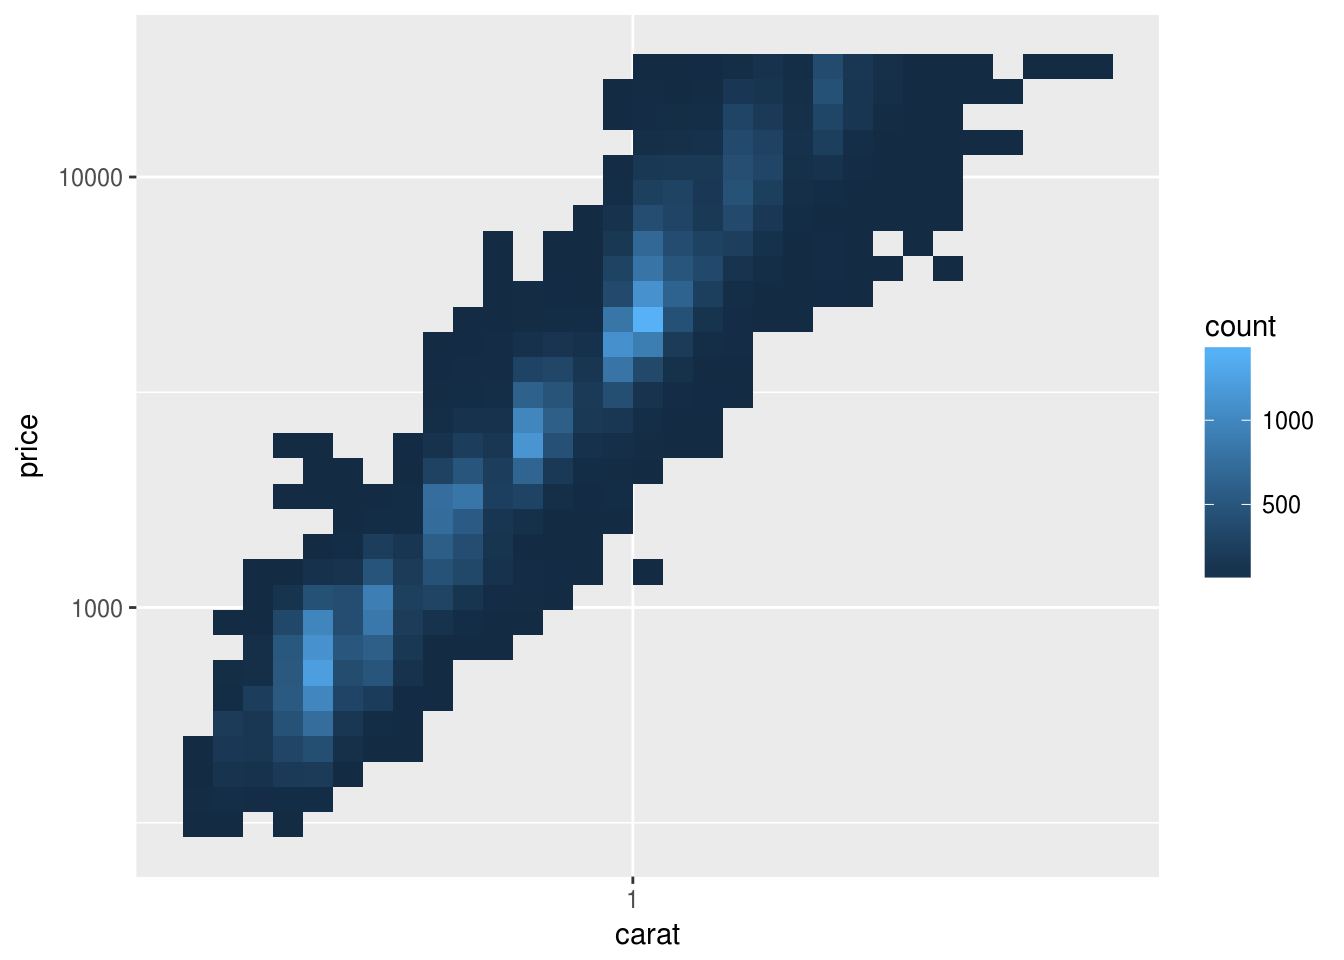
\includegraphics{main_files/figure-latex/unnamed-chunk-138-1.pdf}

\subsection{\texorpdfstring{\texttt{fct\_relevel()} tõstab joonisel osad
tasemed teistest
ettepoole}{fct\_relevel() tõstab joonisel osad tasemed teistest ettepoole}}\label{fct_relevel-tostab-joonisel-osad-tasemed-teistest-ettepoole}

Argumendid on faktor f ja need tasemed (jutumärkides), mida sa tahad
tõsta.

\begin{Shaded}
\begin{Highlighting}[]
\NormalTok{## täiendame eelmist graafikut ümberkorraldatud andmetega}
\NormalTok{p }\OperatorTok{+}\StringTok{ }\KeywordTok{aes}\NormalTok{(tvhours, }\KeywordTok{fct_relevel}\NormalTok{(relig, }\StringTok{"None"}\NormalTok{, }\StringTok{"Don't know"}\NormalTok{))}
\end{Highlighting}
\end{Shaded}

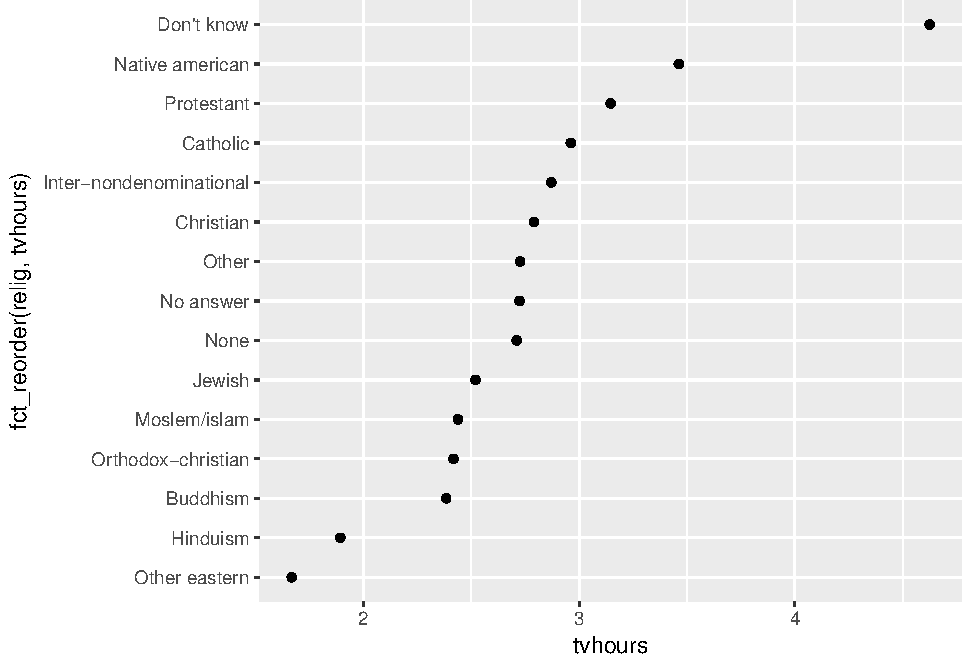
\includegraphics{main_files/figure-latex/unnamed-chunk-139-1.pdf}

\subsection{\texorpdfstring{Joontega plotil saab
\texttt{fct\_reorder2()} abil assotseerida y väärtused suurimate x
väärtustega}{Joontega plotil saab fct\_reorder2() abil assotseerida y väärtused suurimate x väärtustega}}\label{joontega-plotil-saab-fct_reorder2-abil-assotseerida-y-vaartused-suurimate-x-vaartustega}

See muudab ploti paremini jälgitavaks:

\begin{Shaded}
\begin{Highlighting}[]
\NormalTok{## summeerime andmed}
\NormalTok{gsscat_sum <-}\StringTok{ }\KeywordTok{filter}\NormalTok{(gss_cat, }\OperatorTok{!}\KeywordTok{is.na}\NormalTok{(age)) }\OperatorTok
\StringTok{  }\KeywordTok{group_by}\NormalTok{(age, marital) }\OperatorTok
\StringTok{  }\KeywordTok{mutate}\NormalTok{(}\DataTypeTok{N=}\KeywordTok{n}\NormalTok{())}
\NormalTok{## paneme andmed graafikule}
\KeywordTok{ggplot}\NormalTok{(gsscat_sum, }\KeywordTok{aes}\NormalTok{(age, N, }\DataTypeTok{colour =} \KeywordTok{fct_reorder2}\NormalTok{(marital, age, N))) }\OperatorTok{+}
\StringTok{  }\KeywordTok{geom_line}\NormalTok{() }\OperatorTok{+}
\StringTok{  }\KeywordTok{labs}\NormalTok{(}\DataTypeTok{colour =} \StringTok{"marital"}\NormalTok{)}
\end{Highlighting}
\end{Shaded}

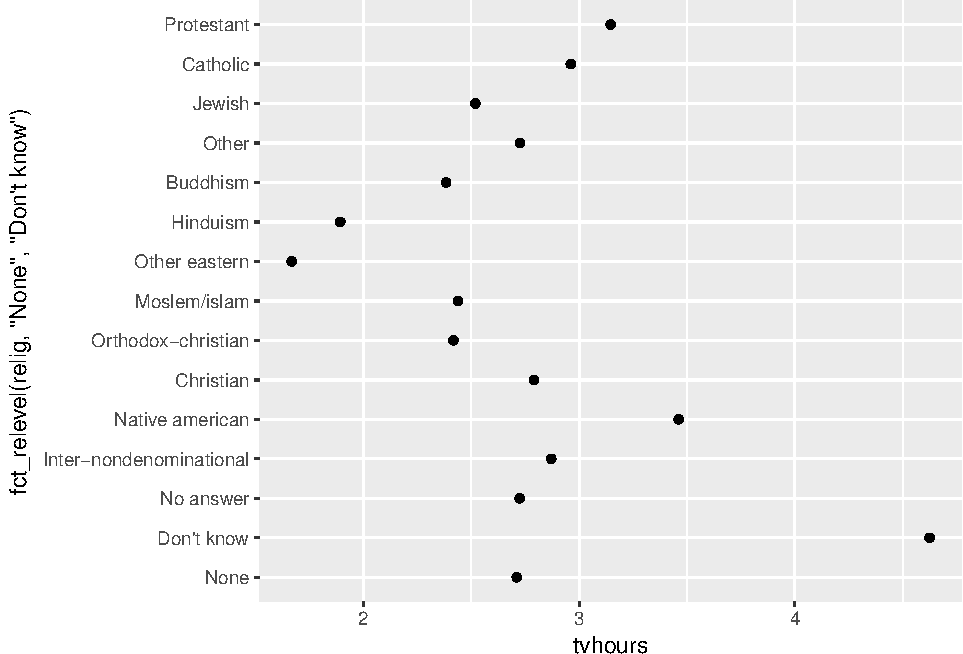
\includegraphics{main_files/figure-latex/unnamed-chunk-140-1.pdf}

\subsection{\texorpdfstring{Tulpdiagrammide korral kasuta
\texttt{fct\_infreq()}}{Tulpdiagrammide korral kasuta fct\_infreq()}}\label{tulpdiagrammide-korral-kasuta-fct_infreq}

Loeme kokku erineva perekondliku staatusega isikud ja paneme need andmed
tulpdiagrammi grupi suurusele vastupidises järjekorras st. väiksemad
grupid tulevad enne.

\begin{Shaded}
\begin{Highlighting}[]
\KeywordTok{mutate}\NormalTok{(gss_cat, }\DataTypeTok{marital =} \KeywordTok{fct_infreq}\NormalTok{(marital) }\OperatorTok\StringTok{ }\KeywordTok{fct_rev}\NormalTok{()) }\OperatorTok
\StringTok{  }\KeywordTok{ggplot}\NormalTok{(}\KeywordTok{aes}\NormalTok{(marital)) }\OperatorTok{+}\StringTok{ }\KeywordTok{geom_bar}\NormalTok{()}
\end{Highlighting}
\end{Shaded}

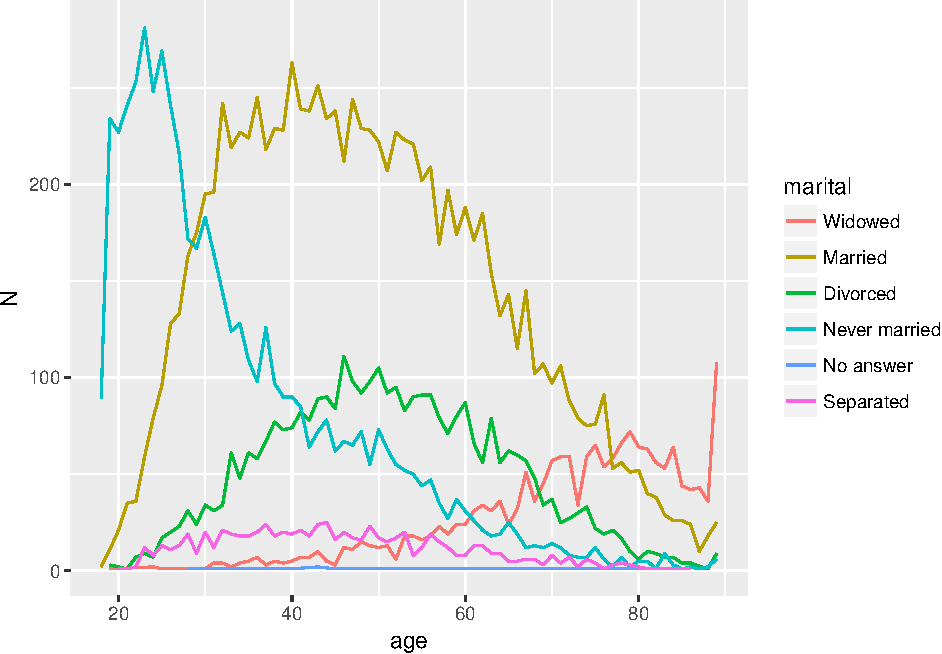
\includegraphics{main_files/figure-latex/unnamed-chunk-141-1.pdf}

\bibliography{packages.bib,book.bib}


\end{document}
